% Supplementary material for the IEEE Transactions on Games version (tog.tex).
% Two builds, as for the paper: supplement.tex is the named build; supplement_review.tex defines \anonbuild.
% Build the paper first (tog_review, with --keep-intermediates), then run tools/build_supplement.py:
% references such as Section~\ref{sec:ep} then print the main text's numbers.
% Sections S1-S11 hold the material moved out of the 10-page version, taken from the long version;
% S12-S16 the full proofs, generated by tools/build_supplement.py (Markdown converted by tools/md2tex.py).
\documentclass[10pt]{article}
\usepackage[margin=2.2cm]{geometry}
\usepackage{amsmath}
\usepackage{amsthm}
\usepackage{unicode-math}
\setmainfont{STIXGeneral}[Path=/System/Library/Fonts/Supplemental/, Extension=.otf, UprightFont=*,
  BoldFont=*Bol, ItalicFont=*Italic, BoldItalicFont=*BolIta]
\setmathfont{STIX Two Math}
\setmonofont{Menlo}[Scale=0.82]
\setsansfont{texgyreheros}[Extension=.otf, UprightFont=*-regular, BoldFont=*-bold]
\usepackage{graphicx}
\usepackage{booktabs}
\usepackage{array}
\usepackage[caption=false,font=footnotesize,labelformat=simple,justification=centering]{subfig}
\usepackage{url}
\usepackage[hidelinks]{hyperref}
% xr is not in the offline bundle: tools/build_supplement.py copies the \newlabel lines of build/tog_review.aux
% into supp/mainlabels.tex, so that \ref to the main text prints the main text's numbers.
\makeatletter\newlabel{sec:intro}{{I}{1}{Introduction}{section.1}{}}
\newlabel{fig:ring}{{1}{2}{Ring $M_{10}$ on the cylinder $\cyl {10}$. (a)~Perspective view; the seam between files j and a (orange) faces the viewer, and the far wall is dashed and faded. Only the pawns that can be seen are drawn: 7 of the 10. (b)~The same position unrolled, with all ten pawns, one per file; file j is next to file a across the dashed seam, and the faded columns repeat j and a. White moves up. The position has value $\nim {2}$ (Section~\ref {sec:star2-rings})}{figure.1}{}}
\newlabel{sec:rules}{{II}{2}{Rules, Values and Conventions}{section.2}{}}
\newlabel{sec:notation}{{\mbox  {II-B}}{2}{Notation}{subsection.2.2}{}}
\newlabel{sec:ep}{{\mbox  {II-D}}{2}{En Passant and the Passed-Pawn Test}{subsection.2.4}{}}
\newlabel{def:epaware}{{1}{2}{E.p.-aware passed pawn}{theorem.1}{}}
\newlabel{fig:basic}{{2}{3}{Basic positions. (a)~Ordinary board: after a2--a4 (arrow) the textbook test calls the a-pawn passed, but b4$\times $a3 en passant removes it; under Definition~\ref {def:epaware} it is not passed. (b), (c)~Cylinder (files a and h adjacent): a zero game and Tiny~1 that use the seam, in all nine settings. Positions of value $1$, $2$, $\star $ and ${\uparrow }$ are in the supplementary material, Section~S1}{figure.2}{}}
\newlabel{thm:cut}{{2}{3}{Cut lemma; \lab {P}, \lab {C2}}{theorem.2}{}}
\newlabel{sec:basic}{{III}{3}{Basic Positions on the Cylinder}{section.3}{}}
\newlabel{fig:trebuchet_2025}{{3(a)}{3}{Subfigure 3(a)}{subfigure.3.1}{}}
\newlabel{sub@fig:trebuchet_2025}{{((a))}{(a)}{Subfigure 3(a)\relax }{subfigure.3.1}{}}
\newlabel{fig:trebuchet}{{3(b)}{3}{Subfigure 3(b)}{subfigure.3.2}{}}
\newlabel{sub@fig:trebuchet}{{((b))}{(b)}{Subfigure 3(b)\relax }{subfigure.3.2}{}}
\newlabel{fig:kinggroup72}{{3(c)}{3}{Subfigure 3(c)}{subfigure.3.3}{}}
\newlabel{sub@fig:kinggroup72}{{((c))}{(c)}{Subfigure 3(c)\relax }{subfigure.3.3}{}}
\newlabel{fig:kings}{{3}{3}{King groups: (a) a tr\'ebuchet on the cylinder (files a and h adjacent) and (b) the tr\'ebuchet T (ordinary board), both real mutual zugzwangs, $0$ when alone; (c) a king group from the 2025 study (cylinder; Section~\ref {sec:sums}) that does not count as $0$: it draws with white to move, a zugzwang for black only}{figure.3}{}}
\newlabel{sec:kings}{{IV}{3}{Kings: The Tr\'ebuchet and When It Is Exact}{section.4}{}}
\newlabel{sec:kings-valid}{{\mbox  {IV-A}}{3}{When Is the Frozen Tr\'ebuchet Exact?}{subsection.4.1}{}}
\newlabel{thm:validity}{{3}{3}{Validity of the convention; \lab {S}}{theorem.3}{}}
\newlabel{cor:v4}{{4}{4}{\lab {S}}{theorem.4}{}}
\newlabel{sec:kings-sweep}{{\mbox  {IV-B}}{4}{How Often Does the Convention Fail?}{subsection.4.2}{}}
\newlabel{tab:puzzles}{{I}{4}{Puzzles of the 2025 Study: Claimed and Exact Values \lab {C2}}{table.1}{}}
\newlabel{sec:sums}{{V}{4}{Sums, Temperature and the Puzzles Revisited}{section.5}{}}
\newlabel{sec:sums-hss}{{\mbox  {V-B}}{4}{When Is the Sum Model Right?}{subsection.5.2}{}}
\newlabel{def:hss}{{5}{4}{Hereditary sum safety}{theorem.5}{}}
\newlabel{thm:hss}{{6}{5}{Sum safety; \lab {S}}{theorem.6}{}}
\newlabel{prop:sumcounter}{{7}{5}{\lab {C2}}{theorem.7}{}}
\newlabel{sec:atlas}{{VI}{5}{The Atlas: What Only the Cylinder Can Do}{section.6}{}}
\newlabel{tab:targets}{{II}{5}{Elkies' Small Values in the Census}{table.2}{}}
\newlabel{fig:eighth}{{4}{5}{Elkies' small values beside T (Fig.~\ref {fig:trebuchet}), each a 10-man position with a legal pawn history (ordinary board). (a)~$1/8$: \pos {W a2 b2 b3 / B a5 a6 b6}. (b)~$\upsec \star $: \pos {W a2 b2 b6 / B a6 b7 c5}. (c)~$\tinyg {1}$: \pos {W a2 b2 b6 / B a6 b7 c6}}{figure.4}{}}
\newlabel{prop:cylonly}{{8}{5}{\lab {C1}}{theorem.8}{}}
\newlabel{sec:targets}{{VII}{5}{Elkies' Small Values}{section.7}{}}
\newlabel{thm:eighth}{{9}{5}{\lab {C2}}{theorem.9}{}}
\newlabel{fig:star2_textbook}{{5(a)}{6}{Subfigure 5(a)}{subfigure.5.1}{}}
\newlabel{sub@fig:star2_textbook}{{((a))}{(a)}{Subfigure 5(a)\relax }{subfigure.5.1}{}}
\newlabel{fig:star2_seven_a}{{5(b)}{6}{Subfigure 5(b)}{subfigure.5.2}{}}
\newlabel{sub@fig:star2_seven_a}{{((b))}{(b)}{Subfigure 5(b)\relax }{subfigure.5.2}{}}
\newlabel{fig:star2_seven_b}{{5(c)}{6}{Subfigure 5(c)}{subfigure.5.3}{}}
\newlabel{sub@fig:star2_seven_b}{{((c))}{(c)}{Subfigure 5(c)\relax }{subfigure.5.3}{}}
\newlabel{fig:star2}{{5}{6}{Positions of the $\nim {2}$ question beside T (Fig.~\ref {fig:trebuchet}; ordinary board). (a)~Candidate: $\nim {2}$ under the textbook test, $\game {2\pm 1}{-2\pm 1}$ under the e.p.-aware test. (b)~Position A and (c)~position B: $\nim {2}$ in the default setting}{figure.5}{}}
\newlabel{sec:star2}{{VIII}{6}{The \texorpdfstring {$\nim {2}$}{*2} Question}{section.8}{}}
\newlabel{thm:census}{{10}{6}{Census; \lab {C2}}{theorem.10}{}}
\newlabel{tab:star2_settings}{{III}{6}{Values of the Candidate and of Positions A and B in the Model Settings}{table.3}{}}
\newlabel{thm:star2seven}{{11}{6}{$\nim {2}$ with seven pawns; \lab {C2}}{theorem.11}{}}
\newlabel{sec:star2-five}{{\mbox  {VIII-D}}{6}{Counts}{subsection.8.4}{}}
\newlabel{sec:star2-rings}{{\mbox  {VIII-E}}{6}{Rings and Higher Nimbers}{subsection.8.5}{}}
\newlabel{fig:least}{{6}{7}{Least number of pawns in a ring of value $\nim {2}$ (steps) and $\nim {3}$ on $\cyl {n}$, in the default setting. Filled markers are computed (\lab {C2} for $\nim {2}$, \lab {C1} for $\nim {3}$), open ones proved for all $n$ as whole-board games \lab {S}; open triangles are upper bounds. The dashed line is one pawn per file. $\nim {3}$ is plotted from $n=10$; ten-pawn $\nim {3}$ rings also exist on $\cyl {7}$ and $\cyl {8}$}{figure.6}{}}
\newlabel{sec:real}{{IX}{7}{From the Model to Real Chess}{section.9}{}}
\newlabel{def:oracle}{{12}{7}{Real-chess oracle value}{theorem.12}{}}
\newlabel{lem:sandwich}{{13}{7}{Sandwich; \lab {P}}{theorem.13}{}}
\newlabel{sec:real-cand}{{\mbox  {IX-A}}{7}{The Textbook Candidate in Real Chess}{subsection.9.1}{}}
\newlabel{thm:oracle-cand}{{14}{7}{Candidate in real chess; \lab {C1}}{theorem.14}{}}
\newlabel{tab:tb}{{IV}{8}{Pawnless Endings Against the Bare King on the Ordinary Board, Cylinder and Torus: Share Won With White to Move and Longest Mate \lab {C2}}{table.4}{}}
\newlabel{sec:real-eighth}{{\mbox  {IX-B}}{8}{Towards a Real-Chess \texorpdfstring {$1/8$}{1/8}}{subsection.9.2}{}}
\newlabel{prop:eighth-real}{{15}{8}{A tablebase-backed oracle value of $1/8$; \lab {C1}}{theorem.15}{}}
\newlabel{sec:tb}{{X}{8}{Mating Without Corners: Tablebases}{section.10}{}}
\newlabel{sec:kpk}{{\mbox  {X-A}}{8}{King and Pawn Against King}{subsection.10.1}{}}
\newlabel{sec:dawson}{{XI}{8}{Dawson's Chess on the Cylinder}{section.11}{}}
\newlabel{fig:dawson_grundy}{{7}{9}{Grundy values $g(n)$ of Dawson's chess on the $3\times n$ ordinary board (octal game $\mathbf {0.137}$), $n\le 80$. Dots mark $g(m)=0$: the $3\times m$ board is a second-player win and the $3\times (m+3)$ cylinder a first-player win (Theorem~\ref {thm:ring})}{figure.7}{}}
\newlabel{eq:dawson}{{1}{9}{Dawson's Chess on the Cylinder}{equation.11.1}{}}
\newlabel{thm:ring}{{16}{9}{Ring rule; \lab {P}, machine-checked for $n\le 22$}{theorem.16}{}}
\newlabel{tab:sf}{{V}{9}{Stockfish~19 at Fixed Depth: Evaluations (\%) Matching the Tablebase, by CGT Class, Without the Seven Decided ($\pm \BIG $) Positions}{table.5}{}}
\newlabel{sec:engines}{{XII}{9}{Engines and Sums}{section.12}{}}
\newlabel{sec:verify}{{XIII}{10}{Verification and Reproducibility}{section.13}{}}
\newlabel{sec:conclusion}{{XIV}{10}{Conclusion and Open Problems}{section.14}{}}
\makeatother
% Shared notation for every section (do not redefine elsewhere)
\newcommand{\BIG}{\mathsf{B}}                       % value of a passed pawn, B = 256
\newcommand{\pos}[1]{\texttt{#1}}                   % pawn list, e.g. \pos{W a2 c2 / B b7 d7}
\newcommand{\fen}[1]{\texttt{\small #1}}
\newcommand{\lab}[1]{\textsf{\footnotesize$\langle$#1$\rangle$}}   % evidence label: \lab{P}, \lab{S}, \lab{C2}, \lab{C1}, \lab{Conj}
\newcommand{\nim}[1]{\mathord{\star#1}}             % nimbers, as in the 2025 paper: \star, \nim{2}
\newcommand{\upsec}{\mathord{\uparrow^{2}}}         % up-second {0 | down star}
\newcommand{\tinyg}[1]{\operatorname{tiny}(#1)}
\newcommand{\game}[2]{\{\,#1 \mid #2\,\}}
\newcommand{\ggame}[2]{\{\,#1 \parallel #2\,\}}
\newcommand{\cyl}[1]{C_{#1}}                        % n-file cylinder
\newcommand{\flatb}[1]{F_{#1}}                      % n-file flat board
\newcommand{\repourl}{https://github.com/aritroBh/cylindrical-chess-cgt}

\newcommand{\anoncodeurl}{anonymized repository link}
\ifdefined\anonbuild
  \newcommand{\codeavail}{available at \anoncodeurl}
  \newcommand{\bytheauthor}{}
  \newcommand{\studyauthor}{Anonymous}
  \newcommand{\studytitle}{Title withheld for review}
\else
  \newcommand{\codeavail}{available at \url{https://github.com/aritroBh/cylindrical-chess-cgt}}
  \newcommand{\bytheauthor}{ by the author}
  \newcommand{\studyauthor}{A.~Bhattacharjee}
  \newcommand{\studytitle}{Analysis of chess endgames on a cylindrical chessboard}
\fi
\renewcommand{\thesection}{S\arabic{section}}
\renewcommand{\thefigure}{S\arabic{figure}}
\renewcommand{\thetable}{S\arabic{table}}
\renewcommand{\thesubfigure}{(\alph{subfigure})}
\makeatletter
\newsavebox{\sf@box}
\newcommand{\sf@setcap}[2][]{\gdef\sf@cap{#2}}
\newcommand{\sf@setlab}[1]{\gdef\sf@lab{#1}}
\newenvironment{subfigure}[2][c]{%
  \gdef\sf@cap{}\gdef\sf@lab{}%
  \begin{lrbox}{\sf@box}\begin{minipage}[#1]{#2}%
  \let\caption\sf@setcap\let\label\sf@setlab}%
  {\end{minipage}\end{lrbox}%
   \ifx\sf@lab\@empty\def\sf@labcmd{}\else\edef\sf@labcmd{\noexpand\label{\sf@lab}}\fi
   \ifx\sf@cap\@empty\subfloat[]{\usebox{\sf@box}\sf@labcmd}%
   \else\subfloat[\sf@cap\sf@labcmd]{\usebox{\sf@box}}\fi}
\makeatother
\theoremstyle{plain}
\newtheorem{theorem}{Theorem}
\renewcommand{\thetheorem}{S\arabic{theorem}}
\newtheorem{lemma}[theorem]{Lemma}
\newtheorem{proposition}[theorem]{Proposition}
\newtheorem{corollary}[theorem]{Corollary}
\newtheorem{conjecture}[theorem]{Conjecture}
\theoremstyle{definition}
\newtheorem{definition}[theorem]{Definition}
\newtheorem{remark}[theorem]{Remark}
\newcommand{\ins}{\operatorname{ins}}
\providecommand{\blacksquare}{\mdlgblksquare}
\newtheorem{wtheorem}{Theorem}   % Section S13 keeps the numbering of its source, proof.tex
\newtheorem{wlemma}{Lemma}
\setcounter{tocdepth}{1}
\makeatletter\renewcommand*\l@section{\@dottedtocline{1}{0em}{2.6em}}\makeatother
\sloppy
\hyphenation{tr\'e-bu-chet tr\'e-bu-chets table-base table-bases}

\begin{document}
\begin{center}
{\Large\bfseries Supplementary Material for\\[2pt]
Combinatorial Game Values and Tablebases for Chess Endgames on a Cylindrical Board}\\[8pt]
\ifdefined\anonbuild Anonymized for review\else Aritro Bhattacharjee\fi
\end{center}

\noindent This supplement belongs to the paper of the same title. References such as ``Theorem~\ref{thm:validity}'' or
``Section~\ref{sec:ep}'' point to the main text; numbers starting with S point to this supplement. Sections S1--S11 hold
the material moved out of the main text: walk-throughs, tables, figures, ring listings and the Forsyth--Edwards
Notation (FEN) of every position with kings. Sections S12--S16 give the full proofs behind the \lab{S} labels, as
written in the project's proof notes. The labels are those of the main text: \lab{P}, proved; \lab{S}, proof
sketched in the main text and given in full here; \lab{C2}, two independently written programs agree; \lab{C1}, one
program; \lab{Conj}, a conjecture. The code and data are \codeavail.

\tableofcontents

\section{Basic Positions and the E.p.-Aware Test}\label{S-basic}
This section holds the walk-throughs of Section~\ref{sec:basic} and the census statistics of Section~\ref{sec:ep} of the main text. Fig.~\ref{fig:basicS} shows the six basic boards; boards (a) and (f) are Fig.~\ref{fig:basic}(b) and (c) of the main text.
\begin{figure}[!htbp]
\centering
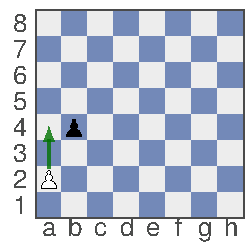
\includegraphics[width=0.30\linewidth]{figures/ep_test.pdf}
\caption{Position \pos{W a2 / B b4} (ordinary board), value $0$. After a2--a4 (arrow) the textbook test calls the
a-pawn passed, but b4$\times$a3 en passant removes it; under Definition~\ref{def:epaware} it is not passed.}
\label{fig:epS}
\end{figure}

% Fig. 2 belongs to Section III; it is defined here so that the full-width float lands next to it.
\begin{figure}[!htbp]
\centering
\begin{subfigure}[t]{0.165\textwidth}\centering
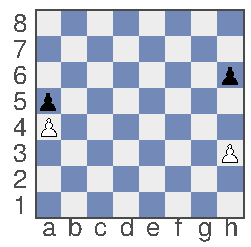
\includegraphics[width=\linewidth]{figures/zero_seam.pdf}
\caption{\pos{W~a4~h3 / B~a5~h6}: $0$}
\end{subfigure}\hfill
\begin{subfigure}[t]{0.165\textwidth}\centering
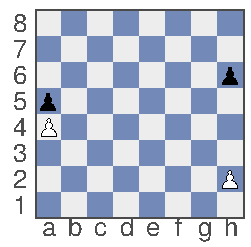
\includegraphics[width=\linewidth]{figures/one.pdf}
\caption{\pos{W~a4~h2 / B~a5~h6}: $1$}
\end{subfigure}\hfill
\begin{subfigure}[t]{0.165\textwidth}\centering
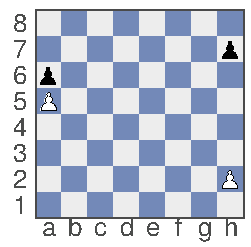
\includegraphics[width=\linewidth]{figures/two.pdf}
\caption{\pos{W~a5~h2 / B~a6~h7}: $2$}
\end{subfigure}\hfill
\begin{subfigure}[t]{0.165\textwidth}\centering
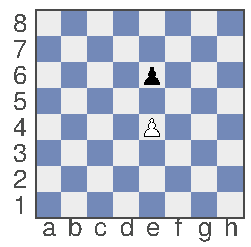
\includegraphics[width=\linewidth]{figures/star.pdf}
\caption{\pos{W~e4 / B~e6}: $\star$}
\end{subfigure}\hfill
\begin{subfigure}[t]{0.165\textwidth}\centering
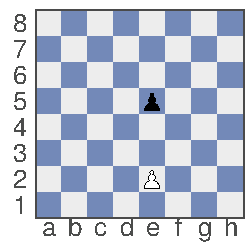
\includegraphics[width=\linewidth]{figures/up.pdf}
\caption{\pos{W~e2 / B~e5}: ${\uparrow}$}
\end{subfigure}\hfill
\begin{subfigure}[t]{0.165\textwidth}\centering
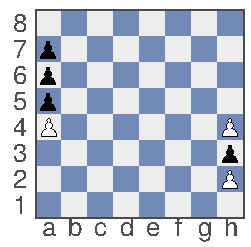
\includegraphics[width=\linewidth]{figures/tiny1_2025.pdf}
\caption{\pos{W~a4~h2~h4 / B~a5~a6~a7~h3}: $\tinyg{1}$}
\end{subfigure}
\caption{Pawn positions with the basic values (cylinder: files a and h adjacent). Each value holds in all nine
settings (Section~\ref{sec:ep}) except in (c), which is $2$ only with e.p.\ on and ${\Uparrow}\star$ with
e.p.\ off.}
\label{fig:basicS}
\end{figure}

One more white pawn makes the difference decisive. In \pos{W~a2~b3 / B~b4} black has no move, and the textbook
test lets white win at once with a2--a4. Under Definition~\ref{def:epaware}, every white move lets black capture
on a3, directly or en passant, and win the race that follows under the count rule, so the value is $0$. Across
the census of Section~\ref{sec:atlas} (all positions with at most six pawns on ordinary boards of width at
most four), the stricter test changes at least $18{,}137$ of the $231{,}071$ values (a few more changes are hidden
where both values exceed the display range), and $4{,}070$ of them in outcome \lab{C1}. The three race rules and three e.p.\ options (textbook test, e.p.-aware test, e.p.\ off) give nine
\emph{settings}. Values use the \emph{default setting} (count rule, e.p.-aware test) unless
stated.

We now build the basic values of Fig.~\ref{fig:basicS} with pawns alone. Each board leaves a file empty, so by
Theorem~\ref{thm:cut} its value is that of an ordinary-board position, cut open along that
file~\cite{Elkies1996,WuYuLandry2010}; in four of them the play crosses the seam. In these examples a move that the
opponent can answer with a passed pawn is a losing move, and it drops out, since having only losing moves is
the same as having no moves at all~\cite{WinningWays,WuYuLandry2010}. A move that the opponent can answer by reaching a
position at least as good for him as the one we started from is \emph{reversible}: in the canonical
form~\cite{WinningWays} it is replaced by the player's moves from that reply, and so drops out when there are
none.

\subsection{The Zero Game}
In the zero game neither player can move: $0=\game{}{}$, a second-player win. In
\pos{W~e4 / B~e5} the two pawns are stuck, so the value is $0$.

Fig.~\ref{fig:basicS}(a) is a zero game that uses the seam. If white goes first, it must play h3--h4, and black
captures across the seam, a5$\times$h4, with a passed pawn. If black goes first, h6--h5 is met by a4$\times$h5.
Whoever moves first loses: again $0$.

\subsection{The Games \texorpdfstring{$1$}{1} and \texorpdfstring{$2$}{2}}
In Fig.~\ref{fig:basicS}(b) the white h-pawn starts one square further back. White can play h2--h3, which leaves
the zero game of (a); the double step h2--h4 only loses the pawn to a5$\times$h4. Black has one move, h6--h5,
and a4$\times$h5 gives white a passed pawn. Thus $G=\game{0}{}=1$.

In Fig.~\ref{fig:basicS}(c) the a-pawns stand one rank higher. White can play h2--h4 or h2--h3, which leave the
games (a) and (b) moved up one rank, $0$ and $1$. Black has only losing moves: h7--h6 is met by
a5$\times$h6, and h7--h5 by a5$\times$h6 en passant across the seam. Thus $G=\game{0,1}{}=2$. With e.p.\
off, h7--h5 is safe and the value falls to an infinitesimal, ${\Uparrow}\star$. Swapping colors and turning the board $180^\circ$ gives $-1$ and
$-2$~\cite{WuYuLandry2010}.

\subsection{The Infinitesimals \texorpdfstring{$\star$, ${\uparrow}$}{Star, Up} and Tiny~1}\label{S-basic-inf}
Star is the game in which both players can move to $0$: $\star=\game{0}{0}$. In Fig.~\ref{fig:basicS}(d),
e4--e5 and e6--e5 each lock the file, so $G=\star$, a first-player win.

Up is ${\uparrow}=\game{0}{\star}$. In Fig.~\ref{fig:basicS}(e), white can play e2--e3, which leaves star, or
e2--e4, which locks the file: $0$. Black can only play e5--e4, which leaves star. Thus
$G=\game{0,\star}{\star}$. Star is reversible for white: black answers e2--e3 with e5--e4, reaching
$0\le G$, since white wins $G$ when black starts. So $G=\game{0}{\star}={\uparrow}$. Up is positive, yet
smaller than every positive number: it is an \emph{infinitesimal}. Switching the colors gives
${\downarrow}=-{\uparrow}$, and we write ${\Uparrow}={\uparrow}+{\uparrow}$.

Tiny~1 is $\tinyg{1}=\ggame{0}{0\mid -1}$, that is, $\game{0}{\game{0}{-1}}$. In Fig.~\ref{fig:basicS}(f), white
can take across the seam, h4$\times$a5, which leaves every pawn blocked: $0$. White's h4--h5 drops out, since
a6$\times$h5 wins for black. Black can only play a5$\times$h4; from there white locks the a-file with a4--a5,
leaving $0$, while black plays a6--a5 and keeps the spare move a7--a6, leaving $-1$. So black's capture leads
to $\game{0}{-1}=-\tfrac12\pm\tfrac12$, and $G=\tinyg{1}$, a positive infinitesimal.

A single file can do more. In \pos{W~a2 / B~a6}, white can play a2--a3, leaving $0$ (either move then leaves
star), or a2--a4, leaving $\star$. Black can only play a6--a5, which leaves the up position of
Fig.~\ref{fig:basicS}(e) on the a-file. So $G=\game{0,\star}{{\uparrow}}$. As in (e), star is reversible for
white, so $G=\game{0}{{\uparrow}}={\Uparrow}\star$, ``double-up star'', one of Elkies'
examples~\cite{Elkies1996}.

\section{Kings: Certificates, Loopy Games and the Failure Sweep}\label{S-kings}
This section holds the parts of Section~\ref{sec:kings} of the main text that were moved out: the certificate theory, the local test for (V2), the loopy games and the details of the failure sweep. Full proofs are in Section~\ref{S-kingsproof}.
\subsection{Certificates}
A local test for (V3) is the \emph{certificate of horizon $h$} of a move in $Z$. Let the punisher answer with a move in $Z$ that does not promote and leaves its king among
the files of $Z$, and call the position then reached $Q$, with the defender to move. (i) With all pawns outside $Z$ removed, the punisher wins the local game: whatever the defender does, and
even if it may pass whenever it is not in check, the punisher (who never passes) promotes or mates with one of its first $h$ moves counted from $Q$, and the defender promotes first
in no play. (ii) With the punisher's king and all pawns in $Z$ removed, and the defender alone to move, no sequence of defender king and pawn moves ends in a promotion within $h$
moves (a king may capture, never steps onto a square attacked by a punisher pawn, and the punisher's other pawns stand still); the defender's pawns in $Z$ fall under (i) (the \emph{counter-promotion condition}). (iii)
The punisher can follow its winning strategy of (i) so that in no play is the defender stalemated before the punisher's $h$-th move. It works in the \emph{promotion game}, where the first promotion wins.

\begin{theorem}[\lab{S}]\label{thm:cert}
In the promotion game, a move in $Z$ with a certificate of horizon $h$ is a loss for its mover, so the
promotion-game analogue of (V3) holds if every move in $Z$, at every position before the first decisive event, has one; for chess, (V3) needs the further
check that a won promotion race is a won game. Clause (ii) cannot be weakened to $h-1$ moves \lab{C1}.
\end{theorem}

In chess small margins fail. On the cylinder with seven files and six ranks, Kb4, Pe4 against Ka1, Pa2 with
white to move, the king move Kb4--c5 has a certificate of horizon~1, yet the chess result after it is a draw, and
Kc5--d5 in Kc5, Pe2 against Ka3, Pc4 on the same board has horizon~2, yet White wins \lab{C1}.

For (V2) we give a sufficient test in the frozen-king game \lab{S} (Proposition~A.19 of Section~\ref{S-kingslong}): the side credited
after a context move that makes a passed pawn wins that game if it has an e.p.-aware passed pawn with a clear
path, the king-safety, escape-square and nearby-pawn conditions of Proposition~A.19 hold, and, with this pawn
removed, no sequence of enemy pawn moves promotes within the enemy turns available before its promoting push. The model looks only at passed pawns: with Pc2, Pd4 against
Pd3 on the $8\times6$ cylinder, black to move, it credits white, yet d3$\times$c2 and c1=Q come first \lab{C1}.

\begin{proposition}[\lab{S}]\label{prop:horizon1}
On boards with at least six ranks, for $h=1$, the counter-promotion condition holds in every chess-legal
context without a passed pawn.
\end{proposition}

\begin{proof}
A pawn that can promote in one move stands on the rank before its last. With six or more ranks it got there by a
single step or a capture, so it cannot be taken en passant, and no enemy pawn can stand ahead of it: it is
already passed.
\end{proof}

\begin{conjecture}[\lab{Conj}]\label{conj:horizon2}
On a board with room for two files beyond the buffer, for every king group whose punishment needs $h\ge2$
moves, some context without a passed pawn leaves a move in the group unpunished.
\end{conjecture}

Real tr\'ebuchets seem to need $h\approx5$--$7$ \lab{Conj}, and a locked pawn pair can still break their zero \lab{C2}. An example: the tr\'ebuchet \pos{W Ka4 b3 / B Kc3 b4} on the cylinder with seven files and six ranks acts as zero in the promotion game beside the locked pair \pos{W e3 / B e4}, but beside the locked pair \pos{W e2 / B e3}, which also has no move and no passed pawn, black to move wins by 1\dots Kd2 instead of losing. Three separately written programs agree; no hand proof is given.

\subsection{Spare King Moves Are Loopy}

A king that can step back and forth without loss gives its side unlimited waiting moves, a loopy
game~\cite{WinningWays,Siegel2013}: $\textsf{on}=\game{\textsf{on}}{}$ if only white can wait,
$\textsf{off}=-\textsf{on}$ if only black can, and $\textsf{dud}$ if both can. Since $\textsf{on}$ exceeds every number, $\BIG$ included, the $\pm\BIG$ convention fails there, and a
decisive event must instead end the game.

\begin{theorem}[Outcomes with spare moves; \lab{S}]\label{thm:loopy}
Let the components form a short game in which every decisive event ends the game, let a side that can wait pass
at any time, and let every other move in $Z$ lose. If only white can wait, black wins exactly when it can force a decisive
event in its favor against a passing white, and white wins otherwise. If both can wait, a side wins exactly when
it can do so against a passing opponent, and otherwise the game is drawn.
\end{theorem}

\begin{proof}[Proof sketch]
If only white can wait, every play is finite, since black's moves are, so the game is determined, and black
wins exactly when some move of black's wins against every white reply, a pass included. If both can wait, a
winning side never needs to pass, so it wins exactly when it can force a decisive event against passes;
otherwise play can go on forever. The full proof is Theorem~A.18a of Section~\ref{S-kingslong}.
\end{proof}

Beside a spare king move, then, component values matter only through their forcing threats. The kings
alone are already loopy: in normal play (a stalemate loses), every quiet K+P against K placement on the boards
from $3\times4$ to $5\times5$, summed with sixteen test games, behaves as a decisive win, $\textsf{on}$,
$\textsf{off}$ or $\textsf{dud}$, or as none of these; none behaves as a number or an infinitesimal, and removing
the edges changes the class of $12.5$--$20.5\%$ of them \lab{C2} (the counts are in \texttt{kings/REPORT.md}, task K4, in the code copy).

\subsection{Details of the Failure Sweep}
We solved, with the kings played out, every component with at most two pawns a side beside a
tr\'ebuchet on boards with six ranks: on one file of the six-file cylinder and of the five-file ordinary board,
and on files d and e of the seven-file cylinder (queen promotions only, at most two queens at a time). Of these, $500$ start without a race and have a determined result. Under the textbook test, $159$ of the $500$ get the wrong outcome \lab{C1}: $107$ through
the kings alone, $18$ through en passant and $34$ because a passed pawn does not win its race. $143$ of the
$159$ are on the seven-file cylinder. The e.p.-aware test repairs the $18$ e.p.\ failures, but the kings undo $13$ of these repairs. On the ordinary $8\times8$ board, in $94$ positions beside a tr\'ebuchet checked against the tablebase, the
convention says all $449$ king moves lose, yet $41$ draw and $7$ win \lab{C1}. The $34$ race failures have one cause: a blocked
enemy pawn steps level with its blocker and promotes first. Ending the game only at a passer that wins the
race by the square rule removes all $52$ convention failures with frozen kings; with real kings $31$ stay repaired, which leaves $128$ mismatches, all from the
kings \lab{C1}. The rule is not sound on every board: on three files, \pos{W a4 b6 / B c7} with black to move passes it, yet black wins. Of the $2{,}154$ $8\times8$ positions beside a tr\'ebuchet whose real results we could compute (not a random sample), $105$ are
draws; in the other $2{,}049$ the model names the winner in $92.5\%$, against $83\%$ and $84\%$ under the mover
and opponent rules \lab{C1}. These positions are the ones our other runs solved, not a sample of a defined class.

Fig.~\ref{fig:f3} shows the agreement rates with Wilson 95\% intervals. The intervals treat positions as independent and so are optimistic.
\begin{figure}[!htbp]
\centering
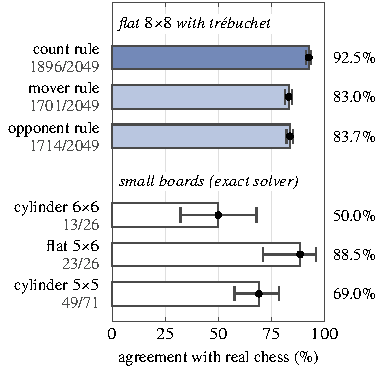
\includegraphics{figures/f3_model_vs_chess.pdf}
\caption{Agreement between the model and real chess, with Wilson 95\% intervals. Top: ordinary $8\times8$ board
beside a tr\'ebuchet, $2{,}049$ decisive positions, by race rule (count rule best). Bottom: exact king-and-pawn
results on small boards.}
\label{fig:f3}
\end{figure}

\section{Sums: The Puzzles and Condition (E)}\label{S-sums}
\subsection{The Two Principles and the Puzzles}
\emph{Principle 1 (number avoidance).} In a sum of numbers and games that are not numbers, a player who can win
can do so without moving in a number~\cite{WinningWays,Siegel2013}.

\emph{Principle 2 (the hottest move).} Move in the component with the highest temperature
(Section~\ref{sec:notation}). For a switch $\game{x}{y}$ between numbers $x>y$, the temperature $(x-y)/2$ is
what each side gains by moving there first, and infinitesimals have temperature $0$. Principle~2 is a
heuristic, not a theorem, but it finds the winning move in every example below.

\begin{figure}[!htbp]
\centering
\begin{subfigure}{0.32\linewidth}\centering
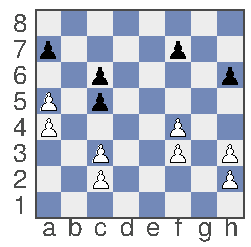
\includegraphics[width=\linewidth]{figures/puzzle71.pdf}
\caption{Puzzle 1}\label{fig:puzzle71}
\end{subfigure}\hfill
\begin{subfigure}{0.32\linewidth}\centering
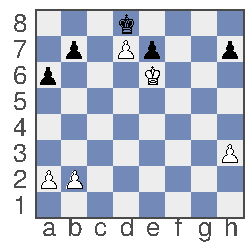
\includegraphics[width=\linewidth]{figures/puzzle72.pdf}
\caption{Puzzle 2}\label{fig:puzzle72}
\end{subfigure}\hfill
\begin{subfigure}{0.32\linewidth}\centering
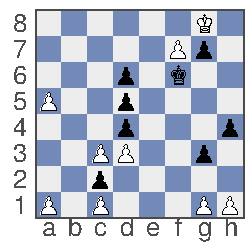
\includegraphics[width=\linewidth]{figures/puzzle73.pdf}
\caption{Puzzle 3}\label{fig:puzzle73}
\end{subfigure}
\caption{Three puzzles of~\cite{Study2025} (cylinder: files a and h adjacent); Table~\ref{tab:puzzles}
gives their exact values. (a)~White wins whoever moves first. (b)~The pawn part is an infinitesimal.
(c)~Puzzle~3 as first drawn: $+\BIG$ (not legal).}
\label{fig:puzzles}
\end{figure}


Table~\ref{tab:puzzles} compares the values first claimed~\cite{Study2025} with the exact ones: the earlier
walk-throughs pick the right winners, but not always the right values.


\emph{Puzzle 1} (Fig.~\ref{fig:puzzle71}) has three components. The earlier values of the c- and f-files are right;
those of files h and a are not. White's a5--a6 still wins
outright, but black, moving first, plays h6$\times$a5 across the seam and leaves $\star$, not a loss, so this
part is $\game{+\BIG}{\star}$, hot, not the number $1$. The total is still a white win whoever moves first, but
play now starts in the h/a component, by far the hottest (Principle~2). White to move plays a5--a6 and wins.
Black to move does best to take on a5 at once, since every other move lets white force a passed pawn (after
h6--h5, a4$\times$h5); white then plays c3--c4 in the next hottest component, and
$1+\star+\game{\game{2}{1}}{0}$ is a white win whoever moves next.

\emph{Puzzle 2} (Fig.~\ref{fig:puzzle72}) has one pawn component, on files h, a and b. The earlier walk-through
finds the right first moves, h3--h4 and a6--a5, and the right outcome, a first-player win. But the value is an
infinitesimal with mean $0$, not $\pm1$, so by Principle~2 it waits until every hot component is settled.
Its king group (Fig.~\ref{fig:kinggroup72}) is not a tr\'ebuchet either. With black to move, the d7 pawn covers
c8 and e8, so Kc7 is forced, and white takes e7 and promotes. With white to move, Kd5, Ke5 and Kf5 all draw:
black wins the d7 pawn, but the white king blockades the e-pawn. The group is a zugzwang for black only, on the
ordinary board \lab{C2} (our solver and the Lichess tablebase) and on the cylinder \lab{C2}, so the real result
of this ten-man position is open.

\emph{Puzzle 3} (Fig.~\ref{fig:puzzle73}) is illegal, with four white pawns on the first rank, and as drawn it
is decided at once, since the pawns on a5 and f7 are passed. On files c and d, white's best move, c3$\times$d4,
leaves $0$. Black's only move, d4$\times$c3, leaves $\game{0}{-1}$: white locks the files with d3--d4, while
black's d5--d4 keeps the spare move d6--d5. Thus $G=\ggame{0}{0\mid -1}=\tinyg{1}$, not $1$, and the legal copy
one rank up, \pos{W c2 c4 d4 / B c3 d5 d6 d7}, has the same value.

\subsection{Condition (E)}
\begin{proposition}[\lab{C1}]\label{prop:condE}
In the pure pawn game, without the passed-pawn rule (play goes on until a side has no move), (E) cannot
be dropped: the sum can be wrong, even in outcome. On the ordinary board with six files and six ranks take
\pos{W a4 f4 / B b4 e5}, where black may take b4$\times$a3 en passant, since white has just played a2--a4. The
whole board is $\game{0}{-4,\,-3\pm2}$, a first-player win, while the sum of its two components is
$\game{-1\star}{-5\star}$, a black win: in the sum the en passant right survives moves in the other component. The two differ
with white to move, as inside larger sums; with black to move, as in the chess position,
both say black wins.
\end{proposition}

\subsection{Two Models}
\emph{Two models.} Our CGT engine computes $S$, as Elkies does~\cite{Elkies1996}, and the independent
whole-board solver $W$. Wherever the two disagree, in every case we tested,
our engine with splitting switched off matches the whole-board solver. The two models agree on every headline value: the $1/8$ and $\upsec\star$
positions of Section~\ref{sec:targets} in all nine settings (Section~\ref{sec:ep}), and the seven-pawn $\nim{2}$
of Section~\ref{sec:star2} in the default setting. Elsewhere they can differ, even in outcome: under the
opponent rule with the e.p.-aware test, \pos{W a3 b3 c2 e2 / B a6 c5 d5 e3} (the first five-file $\nim{2}$ of
Section~\ref{sec:star2-five}) is ${\Uparrow}$ as a sum but $\nim{2}$ on the whole board. Where they differ, we name the model we mean.

\subsection{Two Checks of the Sum Model}\label{S-sumchecks}
Both results of this subsection are computed by one program each \lab{C1}; neither is a proof.

\emph{Sum model against the whole board.} We solved every position without a passed pawn that has at most six
pawns on flat boards three to five files wide, counted up to mirror image and colour swap, in the sum model and on the
whole board ($599{,}098$ positions). We compare only the outcome classes. Table~\ref{tab:censusSW} gives, for each
race rule and passed-pawn test, how often they differ, for all positions, for the hereditarily sum-safe (HSS) ones
and for the others. The default setting is the count rule with the e.p.-aware test.

\begin{table}[!htbp]
\centering
\caption{Positions where the outcome class of the sum model differs from that of the whole board, by passed-pawn
test and race rule: number of differing positions / number of positions.}
\label{tab:censusSW}
\footnotesize
\begin{tabular}{@{}llrrr@{}}
\toprule
test & race rule & all & HSS & not HSS\\
\midrule
textbook & count & $11{,}595$ / $599{,}098$ & $0$ / $539{,}893$ & $11{,}595$ / $59{,}205$\\
textbook & mover & $10{,}496$ / $599{,}098$ & $0$ / $539{,}893$ & $10{,}496$ / $59{,}205$\\
textbook & opponent & $12{,}104$ / $599{,}098$ & $0$ / $539{,}893$ & $12{,}104$ / $59{,}205$\\
e.p.-aware & count & $11{,}300$ / $599{,}098$ & $0$ / $540{,}503$ & $11{,}300$ / $58{,}595$\\
e.p.-aware & mover & $9{,}243$ / $599{,}098$ & $0$ / $540{,}503$ & $9{,}243$ / $58{,}595$\\
e.p.-aware & opponent & $12{,}100$ / $599{,}098$ & $0$ / $540{,}503$ & $12{,}100$ / $58{,}595$\\
\bottomrule
\end{tabular}
\end{table}

\emph{Sum model against real kings.} On the cylinder with eight files and six ranks we fixed the anchors
\pos{Pa3 pa4 Kh4 kb3}, put one component on file d and one on file f with file e empty, and solved the sum with real
kings, queen promotions only, en passant on, and play bounded after the first promotion (the solver's cap~1).
For each side to move the solver returns an upper and a lower bound over W $>$ D $>$ L, from White's point of view; a side is
\emph{exact} if the two agree, and \emph{bounded} otherwise, shown as $[$lower,upper$]$. In
Table~\ref{tab:realkingsum} W, D and L are a win, a draw and a loss for White, and the classes
$\mathcal L$, $\mathcal R$, $\mathcal N$, $\mathcal P$ are the model's, read as white to move, black to move: $\mathcal L$ is
W, W; $\mathcal R$ is L, L; $\mathcal N$ is W, L; $\mathcal P$ is L, W. The anchors alone give exactly this
pattern for $\mathcal P$. The nine P pairs have no passed-pawn component and each contains a locked component of
value $0$, so they test the sum only weakly; the ten N pairs have two live non-passer components of nonzero value.
Of the $38$ sides, $19$ are exact and all agree with the model, and the other $19$ are bounds that contain the model's
result. Every sum of class $\mathcal P$ is bounded on both sides. Bounds confirm nothing beyond that
the model is not contradicted, and all $19$ sums share the same anchors, so the king and anchor placement may matter
at the bound level. One run per position, no independent re-run.

\begin{table}[!htbp]
\centering
\caption{Real-king test of $19$ sums on the cylinder with eight files and six ranks. Components with their values,
the model's outcome class of the sum, and the solver's result with white to move and with black to move.}
\label{tab:realkingsum}
\footnotesize
\setlength{\tabcolsep}{4pt}
\begin{tabular}{@{}lllcll@{}}
\toprule
pair & component on d & component on f & model & white to move & black to move\\
\midrule
P1 & \pos{W d3 / B d4 d5} $(0)$ & \pos{W f2 f4 / B f5} $(1)$ & $\mathcal{L}$ & [D,W] & [D,W]\\
P9 & \pos{W d2 d3 / B d4 d5} $(0)$ & \pos{W f2 f3 / B f4 f5} $(0)$ & $\mathcal{P}$ & [L,D] & [D,W]\\
P21 & \pos{W d2 d4 / B d5} $(1)$ & \pos{W f3 / B f4 f5} $(0)$ & $\mathcal{L}$ & W & W\\
P22 & \pos{W d3 / B d4 d5} $(0)$ & \pos{W f2 / B f4 f5} $(-1/2{\pm}1/2)$ & $\mathcal{N}$ & [D,W] & L\\
P26 & \pos{W d2 d3 / B d4 d5} $(0)$ & \pos{W f2 f3 / B f5} $(1/2{\pm}1/2)$ & $\mathcal{N}$ & W & [L,D]\\
P29 & \pos{W d2 d3 / B d4} $(0)$ & \pos{W f3 / B f4 f5} $(0)$ & $\mathcal{P}$ & [L,D] & [D,W]\\
P35 & \pos{W d2 / B d4 d5} $(-1/2{\pm}1/2)$ & \pos{W f2 f3 / B f4 f5} $(0)$ & $\mathcal{N}$ & [D,W] & L\\
P40 & \pos{W d2 d3 / B d5} $(1/2{\pm}1/2)$ & \pos{W f3 / B f4 f5} $(0)$ & $\mathcal{N}$ & W & [L,D]\\
P48 & \pos{W d2 / B d3 d5} $(-1)$ & \pos{W f2 f3 / B f4} $(0)$ & $\mathcal{R}$ & [L,D] & [L,D]\\
N0 & \pos{W d2 d4 / B d5} $(1)$ & \pos{W f2 / B f3 f5} $(-1)$ & $\mathcal{P}$ & [L,D] & [D,W]\\
N1 & \pos{W d2 d4 / B d5} $(1)$ & \pos{W f2 f3 / B f5} $(1/2{\pm}1/2)$ & $\mathcal{L}$ & W & W\\
N2 & \pos{W d2 d4 / B d5} $(1)$ & \pos{W f2 / B f4 f5} $(-1/2{\pm}1/2)$ & $\mathcal{N}$ & W & [L,D]\\
N3 & \pos{W d2 / B d3 d5} $(-1)$ & \pos{W f2 f3 / B f5} $(1/2{\pm}1/2)$ & $\mathcal{N}$ & [L,W] & [L,D]\\
N4 & \pos{W d2 / B d3 d5} $(-1)$ & \pos{W f2 / B f4 f5} $(-1/2{\pm}1/2)$ & $\mathcal{R}$ & L & L\\
N5 & \pos{W d2 d3 / B d5} $(1/2{\pm}1/2)$ & \pos{W f2 / B f4 f5} $(-1/2{\pm}1/2)$ & $\mathcal{P}$ & [L,D] & [D,W]\\
N6 & \pos{W d2 d3 / B d5} $(1/2{\pm}1/2)$ & \pos{W f2 f3 / B f5} $(1/2{\pm}1/2)$ & $\mathcal{L}$ & W & W\\
N7 & \pos{W d2 / B d4 d5} $(-1/2{\pm}1/2)$ & \pos{W f2 / B f4 f5} $(-1/2{\pm}1/2)$ & $\mathcal{R}$ & L & L\\
N8 & \pos{W d2 d4 / B d5} $(1)$ & \pos{W f2 f4 / B f5} $(1)$ & $\mathcal{L}$ & W & W\\
N9 & \pos{W d2 / B d3 d5} $(-1)$ & \pos{W f2 / B f3 f5} $(-1)$ & $\mathcal{R}$ & L & L\\
\bottomrule
\end{tabular}
\end{table}

\section{The Atlas: Details}\label{S-atlas}
Under the textbook test, the atlas values free of $\BIG$ include just two nimbers: $\star$, and one
$\nim{2}$, the textbook candidate of Section~\ref{sec:star2}, which the e.p.-aware test removes. They also
include several ups, such as ${\Uparrow}\star$ on one file (Section~\ref{S-basic-inf}), and fractions with
denominator at most $4$, of which $3/4$ and $-3/4$ occur only on $\cyl{3}$.

\begin{figure}[!htbp]
\centering
\begin{subfigure}[b]{0.36\linewidth}\centering
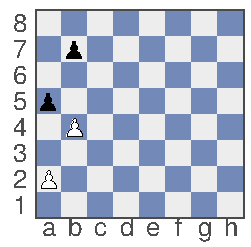
\includegraphics[height=1.1in]{figures/hot3.pdf}
\caption{}
\end{subfigure}\hfill
\begin{subfigure}[b]{0.18\linewidth}\centering
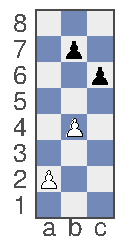
\includegraphics[height=1.1in]{figures/ring3_threequarters.pdf}
\caption{}
\end{subfigure}\hfill
\begin{subfigure}[b]{0.18\linewidth}\centering
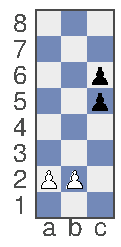
\includegraphics[height=1.1in]{figures/ring3_quarter.pdf}
\caption{}
\end{subfigure}\hfill
\begin{subfigure}[b]{0.22\linewidth}\centering
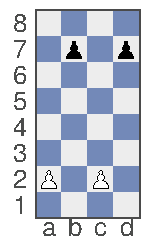
\includegraphics[height=1.1in]{figures/ring4.pdf}
\caption{}
\end{subfigure}
\caption{Atlas values. (a)~The hottest, $\pm3$ (ordinary board). (b)--(d)~Values that occur only on
cylinders (file a next to the last file) under the textbook test: (b)~$3/4$ and (c)~$1/4\pm1/4$ on
$\cyl{3}$, (d)~the $\nim{2}$ candidate's pawns on $\cyl{4}$, not a $\nim{2}$.}
\label{fig:hot3}
\end{figure}

\subsection{The Hottest Position}
Apart from $\pm\BIG$, the highest temperature in the atlas under the textbook test is $3$, reached by white
a2, b4 against black a5, b7 (Fig.~\ref{fig:hot3}(a)). Whoever moves first captures. If white does,
b4$\times$a5 leaves the b7-pawn stuck, since either step lets the a5-pawn through, and white three spare
moves ahead: $3$. If black does, a5$\times$b4 leaves $-3$. Thus $G=\game{3}{-3}=\pm3$ \lab{C1}.

\subsection{Cylinder-Only Values}
A value that occurs on a cylinder but on no ordinary board is \emph{cylinder-only}. By the cut lemma
(Theorem~\ref{thm:cut}) it comes from a ring, which on $n$ files needs $n$ pawns.

\begin{proposition}[\lab{C1}]
Under the textbook test, $53$ atlas values free of $\BIG$ are cylinder-only: $40$ from $3$-file rings and
$13$ from $4$-file rings; the five-pawn rings on $\cyl{5}$ give none. No atlas value occurs only on ordinary boards.
\end{proposition}

On $\cyl{3}$, white a2, b4 against black b7, c6 is $3/4$ and white a2, b2 against black c5, c6 is
$1/4\pm1/4$, under both tests (Fig.~\ref{fig:hot3}(b), (c)). On $\cyl{4}$, the pawn list of the $\nim{2}$
candidate of Section~\ref{sec:star2}, white a2, c2 against black b7, d7, is a different game, since files a and
d are adjacent across the seam: $\game{3/2\pm1/2}{-3/2\pm1/2}$ under the textbook
test but $\game{2\pm1}{-2\pm1}$ under the e.p.-aware test, a value that also occurs on the ordinary board.

Nor are these values robust: the $3$-file ones depend on the race rule ($3/4$ becomes $0$ under the mover
rule), the $4$-file ones on the e.p.\ option. We compared six settings (three race rules, e.p.\ on or off) only for positions with at most
four pawns; among them no value is cylinder-only in all six \lab{C1}.

\section{Elkies\textquotesingle{} Small Values: Details}\label{S-targets}
Theorem~\ref{thm:eighth} of the main text states that the position of its Fig.~\ref{fig:eighth}(a) has value exactly $1/8$.
If white moves first, a2--a4 locks the a-file and leaves the
zero game. The quieter a2--a3 reaches only $\star$, from which black can return to $0$, so it is reversible.
The move b3--b4 is bad, since black's reply leaves $-3$. If black moves first, b6--b5 leaves $1/4$, and
a5--a4 is bad. Thus $G=\game{0}{1/4}=1/8$.

This pawn structure can arise in a game: from the starting position, c2$\times$b3, a7--a5, b7$\times$a6 and
c7$\times$b6 produce it. Its mirror image, white a2, a3, b2 against black a6, b5, b6, cannot, since its
a3-pawn could only have come from a2 or b2, and both are still on their starting squares. The independent
checks were run on the mirror, which has the same value by symmetry: a C solver confirms both parts of the
theorem, and a third, separately written solver confirms the value in all nine settings.

\subsection{Up-Second Star and Tiny~1}
White a2, b2, b6 against black a6, b7, c5 (Fig.~\ref{fig:eighth}(b)) is $\upsec\star$ in all nine settings
\lab{C2}. If white moves first, a2--a4 leaves $0$ and a2--a3 leaves $\star$. If black moves first, a6--a5
leaves ${\downarrow}$. Thus $G=\game{0,\star}{{\downarrow}}=\upsec\star$.

Now move the black c-pawn back to c6 (Fig.~\ref{fig:eighth}(c)). If white moves first, a2--a3 leaves $0$.
If black moves first, a6--a5 leaves $-1/2\pm1/2=\game{0}{-1}$, and c6--c5, which reaches the $\upsec\star$
position, is dominated, since $\game{0}{-1}\le\upsec\star$. Thus $G=\ggame{0}{0\mid -1}=\tinyg{1}$ under
every race rule with en passant on (textbook test \lab{C2}, e.p.-aware test \lab{C1}); with e.p.\ off it is
${\uparrow}$. Unlike the Tiny~1 of Section~\ref{S-basic-inf}, it needs no seam. Both pawn structures
arise from the starting position by c2$\times$b3, b3--b4--b5--b6, a7--a6 and c7--c5 (c7--c6 for Tiny~1).

\subsection{Two Textbook Values That Fail}
Under the textbook test the census also has a $1/8$ at white a2, b2, d2 against black a5, c4, d7 and an
$\upsec$ at white a3, c5, d4 against black a7, b7, d7. The e.p.-aware test makes them $-3/2\pm3/2$ and
$\game{3/4}{{\downarrow}\star}$. Both rested on counting as passed a pawn that
could still be taken en passant. This is why we state Theorem~\ref{thm:eighth} and the $\upsec\star$ above for
all nine settings.

\section{The \texorpdfstring{$\nim{2}$}{*2} Question: Details and Ring Listings}\label{S-star2}
\subsection{The Textbook Candidate}
Fig.~\ref{fig:star2_textbook} shows the candidate \pos{W a2 c2 / B b7 d7} on files a--d. Under the count rule
with the textbook test, it is the only $\nim{k}$ with $k\ge2$ in the census of Section~\ref{sec:atlas}. If white
moves first, a2--a4 leaves $\star$ and c2--c4 leaves $0$; a2--a3 and c2--c3 are worse. The position is symmetric
(turn the board around and swap the colors), so black's d7--d5 leaves $\star$ and b7--b5 leaves $0$. Thus
$G=\game{0,\star}{0,\star}=\nim{2}$.

The weak point is black's plan b7--b5 and b5--b4. After b5--b4 the a-pawn is in the situation of
Fig.~\ref{fig:epS}: the textbook test scores a2--a4 as a passed pawn, $+\BIG$, but in chess black takes
b4$\times$a3 en passant. Under the e.p.-aware test, \pos{W a2 c2 / B b4 d7} is worth $-3$, a black win, so
b7--b5 is worth $-2\pm1$ and, by symmetry, c2--c4 is worth $2\pm1$. The other moves, among them a2--a4 and
d7--d5, which still lead to $\star$, are dominated or reversible. Hence
\[
G=\game{2\pm1}{-2\pm1},
\]
a hot game with mean $0$ and temperature $2$ \lab{C2}.

\subsection{Census and Seven Pawns}
Our CGT engine and an independent C solver, which tests whether $G+\nim{k}$ is a second-player win, agree on
every record, and the independent whole-board solver finds no $\nim{k}$ with $2\le k\le 292$ among
$793{,}299$ labeled placements on widths 1--4 (none reduced by symmetry or translation). Every position in scope has birthday (Section~\ref{sec:notation}) at most $292$, so no
larger nimber can occur. Under the textbook test the census has $6{,}470$ zeros, $3{,}891$ stars and the
candidate; the e.p.-aware test removes that $\nim{2}$. In non-default settings a few other census
positions are $\nim{2}$; Section~\ref{sec:real-cand} tests one of them in real chess.

Both fit beside T, and their pawns can arise in a game: A by a2--a4, b2--b3, c2$\times$d3 and c7--c5, B by
b2--b4, b7$\times$a6, c7--c6 and d7--d5, with g2--g4 and g7--g5 for T; pieces take the other men.

In position A (Fig.~\ref{fig:star2_seven_a}), if white moves first, a4--a5 leaves $0$. The move d3--d4 attacks
c5; every black reply except c5$\times$d4 loses at once, and after c5$\times$d4 white continues b3--b4 to
$\star$, so the reversible move d3--d4 counts as a move to $\star$. White's third move, b3--b4, loses to
c5$\times$b4. If black moves first, a7--a5 leaves $0$ and b7--b6 leaves $\star$. Black's other moves are
reversible: after a7--a6 and b7--b5 white has replies worth $2$ and $3$, both at least $\nim{2}$; and c5--c4
lets d3$\times$c4 free white's d2 pawn for $+\BIG$. Thus
$G=\game{0,\star}{0,\star}=\nim{2}$.

In position B (Fig.~\ref{fig:star2_seven_b}), if white moves first, d2--d4 leaves $0$ and c2--c3 leaves
$\star$. The moves d2--d3 and c2--c4 are reversible, since black's replies reach $-2$ and $-3$, and b4--b5
loses to a6$\times$b5. If black moves first, d5--d4 leaves $0$, and a6--a5 attacks b4: every white reply except
b4$\times$a5 loses at once, and after b4$\times$a5 black continues c6--c5 to $\star$, so a6--a5 counts as a move
to $\star$. Black's third move, c6--c5, loses to b4$\times$c5. Thus $G=\nim{2}$ again. The two analyses
match move for move because B is A with the colors reversed and the files mirrored.

\subsection{Counts, Five Files and Rings}
This subsection gives in full what Sections~\ref{sec:star2-five} and~\ref{sec:star2-rings} of the main text summarize, with every listed ring, count and check.
On ordinary boards of width at most four, in the default setting, two $\nim{2}$ positions, A and B, have seven pawns
and four have eight; one exhaustive scan of $5{,}503{,}282$ root positions gives these counts \lab{C1}, and our
engine re-checked every one \lab{C2}. With
Theorem~\ref{thm:census}, seven is the least number of pawns in a $\nim{2}$ on these boards \lab{C2}. In the
whole-board game, a scan of every position with at most seven pawns on up to nine files extends this to ordinary
boards of any width: a run of empty files acts like one, and every part has pawns of both colors and spans at most
as many files as it has pawns, so six pawns fit on eight files and seven on nine. It finds no $\nim{k}$ with $k\ge2$ with six pawns or fewer, and the only seven-pawn $\nim{2}$ are A and
B \lab{C2}.

On five files a scan of all $14{,}680{,}983$ eight-pawn positions finds $21$ of value $\nim{2}$ in the default
setting \lab{C1}, each using all five files. As whole-board games all $21$ are $\nim{2}$ by two programs \lab{C2};
as sums, $15$ keep the value. Three of the
$21$ come from the $14$ eight-pawn $\nim{2}$ rings on $\cyl{5}$ \lab{C1} by opening them onto files a--e:
\pos{W a3 b3 c2 e2 / B a6 c5 d5 e3}, \pos{W a4 b3 c2 d2 / B a7 b6 c7 e4} and
\pos{W a6 b4 c4 e3 / B a7 c7 d6 e6},
and these are $\nim{2}$ in both models. We call the first \emph{the five-file $\nim{2}$}. No scan here shows a whole-board $\nim{3}$ or higher
\lab{C1}.

By Theorem~\ref{thm:cut} these scans also cover positions with an empty file on $\cyl{3}$ to $\cyl{5}$, which
leaves rings. Two programs' scans of the rings on
$\cyl{5}$ to $\cyl{8}$ with at most eight pawns find $\nim{2}$ in the default setting only in the $14$
eight-pawn rings on $\cyl{5}$ \lab{C2}. Narrower cylinders need fewer pawns. On $\cyl{3}$ the only ring
$\nim{2}$ with six pawns in the default setting is \pos{W a2 a3 b2 / B b7 c6 c7}, and on $\cyl{4}$ the first
are \pos{W a4 b2 c2 / B b6 c5 d6 d7} and its color-reversed twin, with seven; our engine confirms both values
\lab{C2}. No smaller ring on either is a $\nim{2}$: the atlas, a C scan and an independent ring solver agree
\lab{C2}. On $\cyl{6}$ the first rings have nine pawns: a scan of every
nine-pawn ring finds six \lab{C1}, among them \pos{W a4 c4 d2 e2 / B b6 b7 d6 e5 f6}; both programs confirm
three, and the other three are their color-reversed twins \lab{C2}. On $\cyl{7}$ no ring with nine pawns is a
$\nim{2}$, and a third solver written from the rules agrees \lab{C2}; the ten-pawn rings with five pawns a side
include $63$ of value $\nim{2}$ \lab{C1}, such as \pos{W a2 a3 c3 e3 f2 / B a4 b5 d5 f5 g5}, which all three
programs confirm \lab{C2}. So the first ring $\nim{2}$ on $\cyl{n}$ has $n+3$ pawns for $n=3,\dots,7$
\lab{C2}, but on $\cyl{8}$ it has ten: no nine-pawn ring there is a $\nim{2}$ \lab{C2}, while of the ten-pawn
rings $18$ are $\nim{2}$ and two $\nim{3}$, all with five pawns a side \lab{C1}; our engine
confirms each value in both models \lab{C2}, for example \pos{W a3 b3 c3 d2 f2 / B b6 d5 e5 g4 h5}. On $\cyl{9}$
ten is again the least: no nine-pawn ring is a $\nim{2}$, but seven ten-pawn rings are \lab{C2}. From $\cyl{10}$ on, one pawn per file, the least a
ring can have, suffices: \pos{W b2 d2 e3 h3 j5 / B a4 c6 f6 g7 i7} on $\cyl{10}$ and \pos{W c5 e3 h3 i2 k2 / B a4
b7 d7 f7 g6 j6} on $\cyl{11}$ are $\nim{2}$ \lab{C2}, and with pairs of files B4, W2 inserted between files j and a
of the first, or B7, W5 between files a and b of the second, they stay $\nim{2}$ for every $n\le60$ \lab{C2}; on $\cyl{10}$ and $\cyl{11}$ no other ring with $n$ pawns is \lab{C1}.
For proofs we use \emph{walls}: runs of files with one pawn each, alternating in color, the black pawn two
ranks above the white (B4, W2: a black pawn on rank 4, a white one on rank 2); the \emph{window} is the
five or six files, core and adjacent wall files, where the reduced game is played. If a wall pawn moves, its neighbor captures it and gets a passed
pawn, so wall moves lose; with them deleted, inserting a pair of wall files leaves the \emph{reduced game}
unchanged. As a whole-board game this gives a ring $\nim{2}$ with $n+3$ pawns on
every $\cyl{n}$ with $n\ge5$, for example \pos{W b2 c3 c5 d2 f2 h2 / B a5 b5 c6 e4 g4} on $\cyl{8}$ \lab{S}: the
reduced games have $144$ and $104$ positions (odd, even $n$), and two programs check $n<17$ \lab{C2}. As a sum of components, where captures can split the ring, our engine confirms it only
to $n=12$ \lab{C1}. The same argument proves the two families with $n$ pawns above $\nim{2}$ as whole-board games for every
$n\ge10$ \lab{S}, and as sums of components they are $\nim{2}$ on $\cyl{10}$ and $\cyl{11}$ \lab{C1}. The $\cyl{3}$ ring is a $\nim{2}$ with one pawn fewer than any ordinary board of width at most four allows,
and it needs two en passant captures: without black's b4$\times$a3 it is $\uparrow$, without white's
b5$\times$c6 it is $\downarrow$, and with e.p.\ off it is $0$ \lab{C2}.

A $\nim{3}$ lies just beyond these scans, as a single component with nine pawns: B with a white a2 and a black a4 added, \pos{W a2 b4 c2 d2 / B a4 a6 a7 c6 d5}, is $\nim{3}$ on four
files, and so is A with a pair added on file e, \pos{W a4 b3 d2 d3 e4 / B a7 b7 c5 e6}, on five \lab{C2}; A beside a separate group worth
$\star$ on six files is $\nim{2}+\star=\nim{3}$ \lab{C2}. In the whole-board game no position with eight pawns or
fewer on up to eight files, ordinary or cylinder, is $\nim{3}$ \lab{C1}; as sums of components some seven-pawn positions are, but only because a $+\BIG$
cancels a $-\BIG$ (Section~\ref{sec:sums-hss}). With e.p.\ off eight pawns suffice, for example the candidate
beside a group worth $\star$ on six files, \pos{W a2 a4 c2 e2 / B a3 a6 d7 f7}, and the ring \pos{W a5 b3 c2 d2
/ B a7 b5 c6 d4} on $\cyl{4}$ under the opponent rule \lab{C2}. On $\cyl{7}$ the ten-pawn rings above include
eight of value $\nim{3}$, among them \pos{W a2 a5 c4 e2 f2 / B a7 b4 d7 e5 g7}, $\nim{3}$ in both models;
three programs agree on all eight \lab{C2}, and as sums six keep the value. On $\cyl{8}$ the ten-pawn \pos{W a4 c3 d3 e2 g2 / B b7 c6 e5 f5 h4} is $\nim{3}$, and with pairs of files B4, W2
inserted between files b and c it gives, by the same argument, a whole-board $\nim{3}$ with $n+2$ pawns on every
$\cyl{n}$ with even $n\ge8$, and a similar ring does the same for odd $n\ge11$ \lab{S}. One pawn fewer
suffices from $\cyl{11}$ on: no eleven-pawn ring there is $\nim{3}$ \lab{C1}, but the twelve-pawn
\pos{W c4 d6 e3 h3 i2 k2 / B a4 b7 d7 f7 g6 j6} is \lab{C2}, and \pos{W b2 d2 e6 f3 i3 j2 l2 / B a4 c5 e7 g7 h6
k6} on $\cyl{12}$, with pairs of files B4, W2 inserted between files l and a, and a similar ring for odd $n$,
give a $\nim{3}$ with $n+1$ pawns on every $\cyl{n}$ with $n\ge12$, by the wall argument \lab{S}. So $\nim{3}$, like $\nim{2}$, needs no more than eight ranks, but no $\nim{4}$ has turned up: none of
the $134{,}920{,}191$ ten-pawn positions on five files that form one component has a nimber above $\nim{3}$
in the default setting, nor has any of about $24$ million rings, most with at most $11$ files \lab{C1}. A ring with two
cores between walls, whenever it is a nimber, is the nim-sum of its cores \lab{C1}, so a $\nim{4}$ needs a
$\nim{4}$ core.

In the model, then, the $\nim{2}$ question has a positive answer on the ordinary $8\times8$ board: four files
and seven pawns beside T suffice, while Elkies' higher nimbers need larger boards~\cite{Elkies2002}.

\subsection{Rings on the M\"obius Strip}
The strip joins the first and last files with the ranks reversed: square $(n,r)$ is beside $(1,9-r)$. Every pawn
has a direction; white pawns start moving up and black pawns down, and a capture across the seam lands on the
mirrored rank and reverses the direction of the capturing pawn. Double step and promotion follow the direction.
A pawn is passed if no enemy pawn is strictly ahead of it, in its own direction, on its file or a neighboring
file, the seam neighbor being read in mirrored ranks; a pawn that can be taken en passant is not passed. The
whole-board game with the count rule is otherwise that of Section~\ref{sec:star2-rings}. A root ring has a pawn
on every file, no passed pawn and all pawns in their starting directions; rotating the strip does not preserve
this, so rings that differ by a rotation are counted separately.

Table~\ref{tab:mobring} gives the least number of pawns in a root ring $\nim{2}$ and one such ring for each $n$,
in ring notation: one entry per file from the first to the last, the seam lying between the last and the first.
All root rings were scanned for $n=3$ with $3$ to $10$ pawns, $n=4$ with $4$ to $9$, $n=5$ and $6$ with $n$ to
$9$, $n=7$ with $7$ and $8$, and $n=8$ with $8$ (two programs by one AI model agree on every ring). A third
program, written independently from the rules alone, agrees on the eight rings named here, on the number of
root rings, and on the number of $\nim{2}$ rings in every scan below the least, and at the least
for $n=3,4,5,8$ \lab{C2}. Two nine-pawn rings are $\nim{3}$: B67 W4 W2B6 W2B5 W5B7 on five files and
B7 W4 W23 B5 W3B7 W4B7 on six \lab{C2}.

\begin{table}[!htbp]
\centering
\caption{Least number of pawns in a root ring $\nim{2}$ on the M\"obius strip and on the cylinder, with a least ring on the strip.}
\label{tab:mobring}
\begin{tabular}{@{}cccl@{}}
\toprule
$n$ & strip & cylinder & a least ring on the strip\\
\midrule
3 & 6 & 6 & W3B6 W2B7 W4B5\\
4 & 8 & 7 & B5 W23 W2B67 W4B7\\
5 & 6 & 8 & B6 W3 B5 W2 W3B7\\
6 & 8 & 9 & B4 W2 W2 W2B6 B5 W3B7\\
7 & 8 & 10 & B6 W2 W3 B6 B7 W3 W6B7\\
8 & 8 & 10 & B7 W3 W3 B6 W3 B6 B6 W2\\
9 & 10 & 10 & B6 W2 W3 B6 B7 W3 B7 W5 W6B7\\
10 & 10 & 10 & B4 W2 B6 W2 W3 B6 B7 W3 B7 W5\\
11 & 11 & 11 & B4 W2 B6 W2 W3 B6 B7 W3 B7 W5 B7\\
\bottomrule
\end{tabular}
\end{table}

\emph{Nine to eleven files.} For $n=9$, $10$ and $11$ we scanned every root ring with $n$ pawns ($2{,}729{,}517$,
$17{,}146{,}529$ and $109{,}358{,}578$ rings) and, for $n=9$, every root ring with ten pawns ($133{,}597{,}405$ rings).
The two programs agree on every ring \lab{C1}. The independently written program agrees on every $\nim{2}$ and
$\nim{3}$ ring found, and its own scan of the nine-pawn rings on nine files also finds no $\nim{2}$ \lab{C2}. So the
least on nine files is ten pawns. Up to symmetry, ten files have two $\nim{2}$ rings with one pawn per file and
eleven files have one. On nine files one ten-pawn ring is $\nim{3}$: B5 W3 W4 B7 B7 W3 W2 W2B7 B7 \lab{C2}. For
$n=9,10,11$ the strip and the cylinder need the same number of pawns.

\emph{Families.} Three families continue these rings; $(X)^m$ stands for $m$ copies of the block $X$.
\begin{itemize}
\item $(\text{B4 W2})^m$ B6 W2 W3 B6 B7 W3 B7 W5 has $n=2m+8$ files and one pawn per file. It is $\nim{2}$ for
  $m=1,\dots,12$, that is $n=10,\dots,32$.
\item $(\text{B4 W2})^m$ B6 W2 W3 B6 B7 W3 B7 W5 B7 has $n=2m+9$ files and one pawn per file. It is $\nim{2}$ for
  $m=1,\dots,11$, that is $n=11,\dots,31$.
\item B6 W2 W3 B6 B7 W3 $(\text{B7 W5})^m$ W6B7 has $n=2m+7$ files and $n+1$ pawns. It is $\nim{2}$ for
  $m=0,\dots,12$, that is $n=7,\dots,31$.
\end{itemize}
All three families are $\nim{2}$ for every $m$ in these ranges without an upper bound: the first two for every
$m\ge1$ and the third for every $m\ge0$ \lab{S} (Section~\ref{S-star3}, Note~5: a full proof written by one AI model and checked line by line by an AI referee from another vendor). The proof is the insertion
argument of the cylinder (Section~\ref{S-ringn}): two wall files are inserted inside a wall of ten files that does not cross the seam,
and the reduced game does not change. Its base case, the reduced game at $m=5$ ($435$, $417$ and $435$ positions),
was computed by two independently written programs \lab{C2}, which also agree on the members with $m\le13$ solved directly. So one pawn per file
gives a $\nim{2}$ ring on the strip for every $n\ge10$. The members with $m=0$ of the first two
families are not $\nim{2}$, and the eight-file ring of Table~\ref{tab:mobring} is not extended by any block
insertion we tried. Since a ring has at least one pawn per file, the least number of pawns in a ring $\nim{2}$ on the
strip is $n$ for every $n\ge10$. A scan of all root rings with twelve pawns on twelve files was stopped after $50$ of
$128$ parts; the only $\nim{2}$ ring in those parts is the member of the first family.

\subsection{Boards of Other Heights}\label{S-heights}
Everything above is on eight ranks. Here the board has $R$ ranks, $5\le R\le12$: white pawns start on rank $2$,
black pawns on rank $R-1$, and the double step is allowed only from there. We solved single-component positions
without a passed pawn in which every file is occupied (rings, on a cylinder), on ordinary boards of three and four
files and cylinders of three to five files, in increasing number of pawns: about $1.8$ billion positions in all.
Table~\ref{tab:heights} gives the least number of pawns in a $\nim{2}$ and in a $\nim{3}$.

\begin{table}[!htbp]
\centering
\caption{Least number of pawns in a position of value $\nim{2}$ / $\nim{3}$ on a board of $R$ ranks. A dash: every
position of the board was solved and none has the value. ${>}p$: none with up to $p$ pawns; more pawns were not
scanned in full.}
\label{tab:heights}
\small
\begin{tabular}{@{}lcccccccc@{}}
\toprule
board & $R=5$ & $6$ & $7$ & $8$ & $9$ & $10$ & $11$ & $12$\\
\midrule
ordinary, 3 files & -- / -- & 8 / -- & 4 / -- & 10 / -- & 7 / 9 & 7 / 9 & 7 / 9 & 6 / 9\\
ordinary, 4 files & -- / -- & 6 / -- & 4 / 6 & 7 / 9 & 6 / 9 & 8 / 9 & 6 / 8 & 6 / 8\\
$\cyl{3}$ & -- / -- & -- / -- & 4 / -- & 6 / -- & 6 / ${>}12$ & 6 / 10 & 6 / 9 & 6 / 9\\
$\cyl{4}$ & -- / -- & 6 / -- & 6 / ${>}16$ & 7 / ${>}11$ & 6 / ${>}9$ & 7 / ${>}8$ & 6 / ${>}8$ & 6 / ${>}7$\\
$\cyl{5}$ & -- / -- & 8 / -- & 6 / 8 & 8 / ${>}9$ & 6 / 9 & 8 / ${>}8$ & 8 / ${>}7$ & ${>}7$ / ${>}7$\\
\bottomrule
\end{tabular}
\end{table}

No position has a nimber above $\nim{3}$ \lab{C1}. The only nimbers are $0$, $\star$, $\nim{2}$ and $\nim{3}$, with
$831$ positions of value $\nim{2}$ and $77$ of value $\nim{3}$. The least counts are not monotone in the height.
On five ranks no position is $\nim{2}$. On six ranks six pawns are enough, as in \pos{W a2 b2 d2 / B a5 c5 d5} on
four files. On seven ranks four pawns are enough, \pos{W a2 c2 / B c3 b6} on three files, and six pawns make a
$\nim{3}$, \pos{W a2 c2 d3 / B c3 b6 c6} on four files. On the cylinder of three files and nine ranks the position
with all six pawns at home, \pos{W a2 b2 c2 / B a8 b8 c8}, is $\nim{2}$. The column $R=8$ agrees with the counts of
Sections~S6.2 and~S6.3.

The solver was written for this scan. It agrees with our CGT engine on $16{,}000$ random positions, $2{,}000$ for
each height, and on each of the $48$ positions behind a least count in the table \lab{C2}. A third program,
written independently from the rules alone, repeated the complete scans for five ranks, for six ranks and for three
files on seven ranks: $2{,}381{,}595$ positions, with the same number of positions of each nimber and the same least
counts, and no nimber above $\nim{3}$ \lab{C2}. It also showed that the first solver counts $280$ impossible
positions on $\cyl{5}$ with six ranks (twenty pawns, one or two of them white); this changes no entry of the table.
For the other heights, that no smaller position exists and that no $\nim{4}$ occurs rests on the one solver
\lab{C1}. Positions with an empty file, wider boards and more pawns than the table states were not scanned.

\section{From the Model to Real Chess: Details}\label{S-real}
We build the tree under either passed-pawn test, the \emph{textbook tree} or the \emph{e.p.-aware tree}.

\begin{theorem}[Candidate in real chess; \lab{C1}]
For the candidate \pos{W a2 c2 / B b7 d7} beside T (Fig.~\ref{fig:star2_textbook}):
\begin{enumerate}
\item[(a)] In chess the side to move wins; with black to move only 1\ldots~b5 wins; with white to
  move 1.~c4 wins, 1.~a3, 1.~c3 and all king moves lose, and 1.~a4 is unresolved \lab{C2}.
\item[(b)] In the e.p.-aware tree, for every draw treatment, $O$ has left stop $\ge1$ and right stop $\le-1$, so
  it is not $0$ or $\nim{2}$.
\item[(c)] With draws as wins for black, $O=\game{2\pm1}{-2\pm1}$ in both trees.
\end{enumerate}
\end{theorem}

Real chess thus agrees with $\nim{2}$ on the outcome and on every winning first move resolved so far
(1.~a4 is still open), but not on the value: in the e.p.-aware tree, which matches chess, $O$ is hot under every draw treatment, so
the candidate's $\nim{2}$ is a feature of the textbook test, not of chess. In the textbook tree we rule out
$\nim{2}$ only when draws count as wins for black, as in (c), or for white \lab{C1}; with draws worth $0$ we do
not decide it.

A second candidate, \pos{W a3 b3 c2 / B b5 b7 c6} ($10$ men with T), is $\nim{2}$ under the opponent
rule with en passant on (Section~\ref{sec:star2}); its oracle value is positive under every draw treatment
\lab{C1}. The other non-default $\nim{2}$ positions are open.

\subsection{Towards a Real-Chess \texorpdfstring{$1/8$}{1/8}}

The $1/8$ position of Section~\ref{sec:targets} (Fig.~\ref{fig:eighth}(a)) has $10$ men. Its e.p.-aware tree
has $302$ end-position sides with at most seven men, and the tablebase resolves them all. In $290$ of them
only one side has a passed pawn: $283$ agree with the model, $5$ disagree and $2$ are draws; the other $12$ are
races. A search for the larger end positions that decide the value finds five with eight men and three with
nine. Four of the eight-man ones are resolved: seven of their sides agree with the model, and black to move in
\pos{W a3 a5 / B b4 b5} is a black win against it. A second search allows for that result and leaves one
eight-man position and the three of nine men to decide the value. Our king-and-pawn solver (queen promotions
only) shows that all four agree with the model on both sides; the hardest, black to move in
\pos{W b2 b5 / B a5 b4}, needed two promoted queens in the search, $6.1\times10^{10}$ states in $15.6$~h.

\begin{proposition}[A tablebase-backed oracle value of $1/8$; \lab{C1}]
For the $1/8$ position, with queen promotions only in our solver, $O=1/8$, whatever the open end positions do.
\end{proposition}

This $1/8$ assumes the frozen kings of the tree (Section~\ref{sec:kings}); whether the full-chess position
has value $1/8$ is open. The same method applies to $\upsec\star$ and $\tinyg{1}$: their lower bounds already equal the
target values, with $10$ and $12$ end positions of $9$ or $10$ men still open \lab{C1}. Positions A and B have $11$ men beside
T, and the five-file $\nim{2}$ \pos{W a3 b3 c2 e2 / B a6 c5 d5 e3}, which sits legally
beside T, has $12$; no file between its pawns and T is free of pawns, so Theorem~\ref{thm:validity} does not apply. Their oracle values are open: for A and B a
search finds the deciding end positions; the five and seven of them with $8$ men agree with the model
\lab{C2}, but those with $9$ to $11$ men are unsolved, so their $\nim{2}$ is a model value.

\section{Tablebases: Rules and King and Pawn Against King}\label{S-tb}
We now bring in the pieces and ask a classical question: without corners, which material can still force
mate? We computed the tablebases of eight pawnless endings, king and one or two pieces against the bare
king, on the ordinary board, on the cylinder and on the torus, where ranks 1 and 8 are joined as well. Chess
on these boards is an old variant~\cite{Pritchard}. Prose sources say that king and rook cannot force mate
on the cylinder, nor king and queen on the torus~\cite{WikiCylinder,HGMCylinder}; we confirm the torus claim,
but the rook mates from 2.80\% of cylinder positions. We found no earlier tablebase for them.

\emph{Rules.} Pieces move as in Section~\ref{sec:rules} and wrap round each glued edge. There is no castling
and no fifty-move rule, and stalemate and bare kings are draws. A position is legal when the kings are not
adjacent, across the seams included, and the side not to move is not in check. Both dimensions of the board
are even, so the coloring of the squares survives the gluing.

\emph{Verification.} Two retrograde solvers, written independently from these rules, agree on every position
of all 24 tables, about 607 million values with either side to move \lab{C2}. On the ordinary board both
reproduce the known longest mates.



We name endings by their men: KRK is king and rook against king. On the cylinder KQK wins every position, as quickly as on the ordinary board; KRK, KBNK and KNNK do not, and
on the torus not even the queen can force mate (Table~\ref{tab:tb}).

\emph{KRK and KBNK rarely force mate on the cylinder.} The first and eighth ranks are still edges, but now
closed loops with no corner. The rook wins only 2.80\% of the positions, all from mating nets already
in place, such as Ka3, Rb2 against Ka1: 1.~Rb3 Kh1 2.~Rg3 Ka1 3.~Rg1\#. The rook covers h1 and the
white king h2, the two flight squares across the seam. Bishop and knight win even more rarely: their mate
needs a corner of the bishop's color, and the cylinder has none.

\emph{Bishops on opposite colors win every position on the cylinder}, and faster than on the ordinary board,
although the bishop pair is said not to mate there~\cite{HGMCylinder}.
Here the seam helps the attacker: every diagonal winds round from the first rank to the eighth. The longest
line ends in Ke6, Be1, Bf1 against Ke8: the bishop on f1 checks along f1--h3--a4--e8, across the seam, and
the bishop on e1 covers d8 and f8.

\emph{On the torus, of the eight endings, only KRRK and KQRK force mate}, and they win from every position. KRBK wins only where
a mate in one is already set up, and the bishop pair has mating positions that no legal white move can
produce.

\emph{Twisted boards.} KRK wins everywhere on the M\"obius strip (files a and h joined, ranks reversed), but
only $0.66\%$ on the Klein bottle, which also joins ranks 1 and 8 \lab{C2}.


\subsection{King and Pawn Against King}
We solved every legal KPK position on the $8\times8$ ordinary board and cylinder twice, with our
king-and-pawn solver of Section~\ref{sec:kings} (all four promotions) and with a separately written KPK
solver (queen promotion only). They agree on all 326,640 cylinder positions and differ on exactly 6
ordinary-board positions, where only a rook promotion wins, such as Ka4, Pb7 against
Ka6 \lab{C2}. Table~\ref{tab:kpk} gives the counts; the cylinder has fewer legal positions, since across the seam
the kings may not touch and, with white to move, the pawn may not attack the black king.

\begin{table}[!htbp]
\centering
\caption{King and Pawn Against King: Legal Positions and White Wins on the $8\times8$ Ordinary Board and
Cylinder \lab{C2}}
\label{tab:kpk}
\footnotesize
\begin{tabular}{@{}lrrrr@{}}
\toprule
& \multicolumn{2}{c}{White to move} & \multicolumn{2}{c}{Black to move} \\
\cmidrule(lr){2-3}\cmidrule(l){4-5}
Board & Legal & White wins & Legal & White wins \\
\midrule
Ordinary & 163,328 & 124,960 & 168,024 & 97,604 \\
Cylinder & 160,656 & 126,736 & 165,984 & 92,760 \\
\bottomrule
\end{tabular}
\end{table}

\begin{figure}[!htbp]
\centering
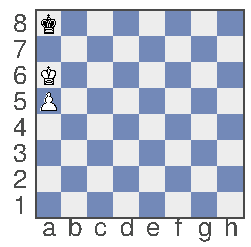
\includegraphics[width=0.26\linewidth]{figures/kpk_rookpawn.pdf}
\caption{Ka6, Pa5 against Ka8, with either side to move: a white win on the cylinder (files a and h adjacent),
a draw on the ordinary board.}
\label{fig:kpk_rookpawn}
\end{figure}

Fig.~\ref{fig:kpk_rookpawn} shows the classic rook-pawn draw: on the ordinary board the black king cannot be
driven out of the corner without stalemate. On the cylinder we may shift every man four files to the right,
which gives Ke6, Pe5 against Ke8, the textbook win whoever is to move. Back on the a-file, with black to move,
play goes 1\ldots~Kb8 2.~Kh7 Kb7 3.~a6+, and the pawn promotes under the king, which guards a7 and a8 from h7.

Of the positions legal on both boards, 16,538 ordinary-board draws become cylinder wins. The seam also
helps the defender, since a king on the h-file now stands beside an a-pawn: 15,930 ordinary-board wins
become cylinder draws. Zugzwang, the engine of the tr\'ebuchet, is more common on the cylinder: 216
reciprocal zugzwangs (white to move draws, black to move loses) against 160 on the ordinary board
\lab{C2}.

\begin{table}[!htbp]
\centering
\caption{King and Pawn Against King on $\cyl{n}$: White-to-Move Wins and Reciprocal Zugzwangs \lab{C2}}
\label{tab:oddw}
\footnotesize
\begin{tabular}{@{}lrrr@{}}
\toprule
$n$ & Legal, white to move & White wins (\%) & Reciprocal zugzwangs \\
\midrule
3 & 5,706   & 53.00 & 0   \\
4 & 16,008  & 65.87 & 208 \\
5 & 34,350  & 73.92 & 95  \\
6 & 63,036  & 76.55 & 132 \\
7 & 104,370 & 77.49 & 175 \\
8 & 160,656 & 78.89 & 216 \\
\bottomrule
\end{tabular}
\end{table}

\emph{Other widths.} Table~\ref{tab:oddw} covers $\cyl{n}$ for $n=3,\dots,8$, where two independently
written solvers agree \lab{C2}; one widened solver gives 79.41\% and 79.94\% for $n=9,10$ \lab{C1}. Odd
and even widths behave alike: the win rate rises with $n$, and from $n=4$ on the share of reciprocal zugzwangs falls,
from 1.30\% to 0.13\% at $n=8$. The tr\'ebuchet of Fig.~\ref{fig:trebuchet_2025} is a mutual zugzwang for $4\le n\le8$ \lab{C2} and $n=9$ \lab{C1}, and illegal on $\cyl{3}$. Ka3, Pa2 against
Ka5, a draw on the ordinary board, is a reciprocal zugzwang for $4\le n\le8$ \lab{C2} and $n=9,10$ \lab{C1}. On $\cyl{3}$, Ka1, Pa7 against Ka3
wins at once: a8=Q checks along the a-file, which covers a4, and the wrapped diagonals and the white king cover
the other flight squares \lab{C2}.

\emph{A pawn each.} With all promotions but at most one new piece, our solver decides 89\% of the 14.6 million
KPKP placements on the cylinder (14.9 million on the ordinary board) and 83\% on the ordinary board \lab{C1}
(placements with an e.p.\ right pending are not enumerated). Of the positions decided on both,
10\% change result, three quarters of them to a draw, and 576 pairs of reciprocal zugzwangs exist only on the
cylinder, 20 of them mutual: in Ka3, Ph2 against Kg2, Ph3 whoever moves loses, since Ka3 reaches the
locked pawns across the seam; a second solver agrees on a sample \lab{C2}.

\section{Dawson\textquotesingle{}s Chess: Details and Learning}\label{S-dawson}
\begin{figure}[!htbp]
\centering
\begin{subfigure}{0.48\linewidth}
\centering
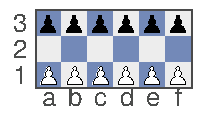
\includegraphics[scale=0.8]{figures/dawson_strip.pdf}
\caption{}
\label{fig:dawson_strip}
\end{subfigure}\hfill
\begin{subfigure}{0.48\linewidth}
\centering
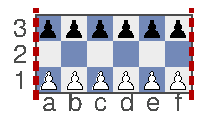
\includegraphics[scale=0.8]{figures/dawson_ring.pdf}
\caption{}
\label{fig:dawson_ring}
\end{subfigure}
\caption{Starting position of Dawson's chess on six files. (a) $3\times6$ ordinary board. (b) $3\times6$
cylinder: files a and f are adjacent; dashed edges are glued.}
\label{fig:dawson_boards}
\end{figure}

\emph{Rules.} Dawson's chess~\cite{Dawson1935} is played on a $3\times n$ board
(Fig.~\ref{fig:dawson_boards}) with white pawns on rank~1, black pawns on rank~3 and rank~2 empty. Pawns move
and capture as in chess, captures are compulsory, and no pawn can double-step or promote. The last player to
move wins; in the mis\`ere form that Dawson posed, the last player loses.

Call a file \emph{untouched} if both its pawns stand on their starting
squares. Suppose white plays c1--c2 with the b- and d-files untouched. The pawn on c2 attacks b3 and d3, so
black must capture, say b3$\times$c2. That pawn attacks b1 and d1, so white must recapture, say
d1$\times$c2, and then come d3$\times$c2 and b1$\times$c2. This leaves black to move, with the b- and
d-files empty and the c-file blocked for good, since a pawn enters a file only by capturing. At the end of a
row the push takes three plies and empties its one neighbor; a push with no untouched neighbor is
blocked.

Each such sequence is forced and touches only the pushed file and its neighbors. Counting a whole sequence as
one move, strips separated by empty files never interact, and both players have the same sequences, so this
game of sequences is impartial. A strip of $n$ untouched files is therefore the octal game $\mathbf{0.137}$~\cite{GuySmith1956,WinningWays},
in which a move removes a file and its untouched neighbors. Its Grundy values are $g(0)=0$, $g(1)=1$ and,
for $n\ge2$,
\begin{equation}
g(n)=\operatorname{mex}\bigl(\{g(n-2)\}\cup\{g(a)\oplus g(b) : a+b=n-3\}\bigr),
\end{equation}
where $a,b\ge0$, $\oplus$ is the nim-sum and mex the least non-negative integer not in the set. The first
player wins the ordinary $3\times n$ board exactly when $g(n)\ne0$. The values from~\eqref{eq:dawson}
have period 34 with last exception $n=51$~\cite{GuySmith1956}, which two programs reproduce for $n\le300$
\lab{C2}.

\emph{What was wrong.} In~\cite{Study2025} a pawn could be removed from a single row only when
both its neighbors were empty, so a full row of two or more pawns has no move. Its recurrence lacks the
end-file term $g(n-2)$ of~\eqref{eq:dawson} and the value $g(1)=1$, agrees with $g$ at only 31 of the 301 values
$n\le300$, and gives the wrong cylinder outcome for 56 of them \lab{C2}. The first is $n=4$, a predicted
first-player win: white's push and four captures leave one untouched file, black pushes that pawn, it is
blocked, and white has no move.

\emph{Mis\`ere play.} A forced sequence has odd length and ends with the player who began it, so the
ring rule carries over: the first player wins the mis\`ere cylinder exactly when the strip of $n-3$ files is
a mis\`ere P-position. Our implementation of the Plambeck--Siegel algorithm~\cite{PlambeckSiegel2008}
reproduces their partial quotient for strips of at most 32 files (order 638, 109 P-positions) and agrees
with exhaustive search on 7.4 million positions \lab{C2}; the next quotient did not finish.

\emph{A warning about sums.} As a partizan game on its own, the ordinary $3\times5$ board is $\star$,
although $g(5)=3$. The outcome agrees, but only $g$ adds up: a sum of such values would let a player reply
elsewhere while a capture is pending.

\emph{The machine check of Theorem~\ref{thm:ring}.} A program that plays the pawn rules directly (\texttt{dawson/pawnboard.py} in the code copy, record \texttt{dawson/pawnboard\_16.txt}) builds every position of the full ring for $3\le n\le16$. For each $n$ and each side to move first, the outcome in normal and in mis\`ere play is the one the ring rule gives \lab{C1}.
\subsection{Learning Dawson\textquotesingle{}s Chess}
In normal-play Dawson's chess the first player wins exactly when the strips' Grundy values have a nonzero
nim-sum~\cite{GuySmith1956,WinningWays}. A long short-term memory (LSTM) value network in PyTorch~\cite{PyTorch}, trained on total lengths up to
$30$, scores $0.82$ on lengths $31$--$80$, against $0.79$ for the majority guess \lab{C1}; the rule scores $1.0$,
and linear probes on the strip embedding do no better than the majority guess.

\section{Further Open Problems}\label{S-open}
The main text lists four open problems; this is the full list of six.
\begin{enumerate}
\item \emph{A certified $1/8$.} With queen promotions and frozen kings the oracle value is exactly $1/8$. Do
  the decisive end positions keep their results with all four promotions (Section~\ref{sec:real-eighth})?
\item \emph{The seven-pawn $\nim{2}$ in real chess.} The 8-man end positions deciding A and B agree with the
  model; those with 9 to 11 men are unsolved
  (Section~\ref{sec:real-eighth}).
\item \emph{Higher nimbers.} The least number of pawns in a ring $\nim{2}$ on $\cyl{n}$ is $n+3$ for $3\le n\le7$,
  ten for $7\le n\le10$ \lab{C2} and $n$ for every $n\ge10$ as a whole-board game \lab{S}. For $\nim{3}$ it is $n+2$ on $\cyl{10}$, $n+1$ on $\cyl{11}$ and $\cyl{12}$ \lab{C1} and at
  most $n+1$ for every $n\ge12$ \lab{S}: can it be $n$? Are the wall
  families $\nim{2}$ as sums for all $n$? Is there a $\nim{4}$ at any height?
\item \emph{When is a tr\'ebuchet zero?} Theorem~\ref{thm:cert} settles the promotion game, not chess: find a
  local test for chess, or settle Conjecture~\ref{conj:horizon2} (real tr\'ebuchets seem to need $h\approx5$--$7$).
\item \emph{Endgames without edges.} With at most one new piece, $11\%$ of KPKP positions on the cylinder
  stay undecided, and KPPK comes next. On the M\"obius strip the least ring $\nim{2}$ is known for $n\le11$
  (Section~S6.4) and one pawn per file suffices for $n\ge10$ (Section~S15); the least for $n\ge12$ and the kings remain open.
\item \emph{Mis\`ere Dawson's chess.} Dawson asked about mis\`ere play \cite{Dawson1935}: is the mis\`ere
  quotient \cite{PlambeckSiegel2008} of Dawson's chess infinite? By the ring rule (Theorem~\ref{thm:ring}), an
  answer for strips also answers the cylinder.
\end{enumerate}

\section{Positions with Kings in FEN}\label{S-fen}


Table~\ref{tab:positions} gives the FEN of each main position with kings. A men list gives the white men, then
the black men; K marks a king. On ``$\flatb{8}$+T'' the position stands on the ordinary
$8\times8$ board beside T (Fig.~\ref{fig:trebuchet}), and its FEN includes T. FENs give the piece placement
only; white is to move unless stated, and values are in the default setting (Section~\ref{sec:ep}). Pawn-only
positions are given by their pawn lists.

\begin{table}[!htbp]
\centering
\caption{Main Positions with Kings}
\label{tab:positions}
\footnotesize
\setlength{\tabcolsep}{4pt}
\begin{tabular}{@{}>{\raggedright\arraybackslash}p{0.27\textwidth}p{0.05\textwidth}%
  >{\raggedright\arraybackslash}p{0.255\textwidth}>{\raggedright\arraybackslash}p{0.335\textwidth}@{}}
\toprule
Role and value & Board & Men (white / black) & FEN \\
\midrule
\multicolumn{4}{@{}l}{\emph{Kings and puzzles}} \\
Tr\'ebuchet across the seam & $\cyl{8}$ & \pos{W Kh5 a4 / B Kb4 a5} &
\fen{8/8/8/p6K/Pk6/8/8/8} \\
Tr\'ebuchet T & $\flatb{8}$ & \pos{W Kf5 g4 / B Kh4 g5} & \fen{8/8/8/5Kp1/6Pk/8/8/8} \\
Puzzle~2 king group: white to move draws & $\cyl{8}$ & \pos{W Ke6 d7 / B Kd8 e7} &
\fen{3k4/3Pp3/4K3/8/8/8/8/8} \\
Puzzle~2: pawns infinitesimal, mean $0$ & $\cyl{8}$ & \pos{W Ke6 a2 b2 d7 h3 / B Kd8 a6 b7 e7 h7} &
\fen{3k4/1p1Pp2p/p3K3/8/8/7P/PP6/8} \\
\midrule
\multicolumn{4}{@{}l}{\emph{Elkies' small values}} \\
$1/8$, in all nine settings & $\flatb{8}$+T & \pos{W a2 b2 b3 / B a5 a6 b6} &
\fen{8/8/pp6/p4Kp1/6Pk/1P6/PP6/8} \\
$\upsec\star$, in all nine settings & $\flatb{8}$+T & \pos{W a2 b2 b6 / B a6 b7 c5} &
\fen{8/1p6/pP6/2p2Kp1/6Pk/8/PP6/8} \\
Tiny~1 & $\flatb{8}$+T & \pos{W a2 b2 b6 / B a6 b7 c6} & \fen{8/1p6/pPp5/5Kp1/6Pk/8/PP6/8} \\
Textbook $1/8$, now $-3/2\pm3/2$ & $\flatb{8}$+T & \pos{W a2 b2 d2 / B a5 c4 d7} &
\fen{8/3p4/8/p4Kp1/2p3Pk/8/PP1P4/8} \\
Textbook $\upsec$, now $\game{3/4}{{\downarrow}\star}$ & $\flatb{8}$+T & \pos{W a3 c5 d4 / B a7 b7 d7} &
\fen{8/pp1p4/8/2P2Kp1/3P2Pk/P7/8/8} \\
\midrule
\multicolumn{4}{@{}l}{\emph{The $\nim{2}$ question}} \\
Candidate: $\game{2\pm1}{-2\pm1}$; textbook $\nim{2}$ & $\flatb{8}$+T &
\pos{W a2 c2 / B b7 d7} & \fen{8/1p1p4/8/5Kp1/6Pk/8/P1P5/8} \\
Second candidate: opponent-rule $\nim{2}$, oracle $>0$ & $\flatb{8}$+T &
\pos{W a3 b3 c2 / B b5 b7 c6} & \fen{8/1p6/2p5/1p3Kp1/6Pk/PP6/2P5/8} \\
Position A: $\nim{2}$ & $\flatb{8}$+T & \pos{W a4 b3 d2 d3 / B a7 b7 c5} &
\fen{8/pp6/8/2p2Kp1/P5Pk/1P1P4/3P4/8} \\
Position B: $\nim{2}$ & $\flatb{8}$+T & \pos{W b4 c2 d2 / B a6 a7 c6 d5} &
\fen{8/p7/p1p5/3p1Kp1/1P4Pk/8/2PP4/8} \\
Five-file $\nim{2}$ & $\flatb{8}$+T & \pos{W a3 b3 c2 e2 / B a6 c5 d5 e3} &
\fen{8/8/p7/2pp1Kp1/6Pk/PP2p3/2P1P3/8} \\
\midrule
\multicolumn{4}{@{}l}{\emph{Real chess}} \\
Last $1/8$ end position: white wins (queens only) & $\flatb{8}$+T &
\pos{W b2 b5 / B a5 b4} & \fen{8/8/8/pP3Kp1/1p4Pk/8/1P6/8} \\
$1/8$ end position against the model: black to move wins & $\flatb{8}$+T &
\pos{W a3 a5 / B b4 b5} & \fen{8/8/8/Pp3Kp1/1p4Pk/P7/8/8} \\
KPK rook pawn: cylinder win, ordinary draw & $\cyl{8}$ &
\pos{W Ka6 a5 / B Ka8} & \fen{k7/8/K7/P7/8/8/8/8} \\
\bottomrule
\end{tabular}
\end{table}

\clearpage
\section{Full Proofs: Validity of the Convention, Sums, Certificates and Loopy Games}\label{S-kingsproof}
% Section S12, first subsection: the four results marked S in Sections 4 and 5 of the main text,
% with every definition they need and complete hand proofs. Results are numbered A.1, A.2, ... by hand.
\subsection{The Four Main Results, Self-Contained}\label{S-core}

This subsection states and proves the four results of the main text that carry the label S: Theorem~\ref{thm:validity},
Corollary~\ref{cor:v4}, the certificate statement of Section~\ref{sec:kings-valid} and Theorem~\ref{thm:hss}. It can be
read without the rest of this section. All definitions are given here, and every proof is a hand proof that uses only
these definitions and earlier steps of this subsection. No step rests on a computation. The one computed statement we
quote (part (c) of Proposition~A.14) is marked as such and is used nowhere. Numbered items are A.1, A.2, and so on.
We assume the basic theory of short games: disjunctive sums, outcome classes, and Zermelo's theorem that a finite game
without draws has a winner~\cite{Siegel2013}.

\subsubsection*{A.I Board, pawns and passed pawns}

\textbf{Board.} The board has $n$ files and $H\ge 3$ ranks. (On three ranks every pawn is passed, so the results below are about the empty position only; on four ranks a double step
promotes and no e.p.\ capture is possible.) It is \emph{flat} (files $1,\dots,n$ in a row) or a
\emph{cylinder} (file $n$ is also next to file $1$). The \emph{distance} of two files is their distance in the row, or
on the cycle for the cylinder. White pawns move up, black pawns down. A square is \emph{ahead} of a white pawn if its rank is higher than the pawn's, and ahead of a black pawn if
its rank is lower. No pawn stands on its own first rank; since pawns only move forward, this holds in all play. In this subsection a position holds pawns and at most two
kings, and no other piece until a promotion.

\textbf{Pawn moves.} A pawn steps one square forward to an empty square; from its own second rank it may instead
\emph{double step} two squares forward over an empty square to an empty square; it captures an enemy pawn diagonally
forward on a file at distance $1$ (across the seam on the cylinder). If the last move was a double step of a pawn $q$ from
$a$ over $b$ to $c$, an enemy pawn on the square beside $c$ (same rank, file at distance $1$) may capture \emph{en passant}
(e.p.): it moves to $b$ and $q$ is removed. This is allowed on the next move only. The position then carries a
\emph{right}; the right is \emph{usable} if such an enemy pawn exists. A pawn that reaches its last rank promotes; in the pawn games $W$ and $S$
below it stays there as a pawn, as in our engine. Kings are
never captured.

\textbf{A.1 Lemma (files).} \emph{A pawn changes file only by a capture, and it then lands on a file that held an enemy
pawn just before the move. Hence, in play in which kings are the only pieces other than pawns (all play in $W$, $S$, the
move bound and the threats below, where a promoted pawn stays a pawn, and chess before the first promotion), no pawn ever
enters a file that holds no pawn.}

\begin{proof}
A step or double step keeps the file. A capture lands on the square of the captured pawn; an e.p.\ capture lands on $b$,
on the file of the captured pawn $q$. Kings are never captured, so in such play the only capturable pieces are pawns.
\end{proof}

\textbf{Components.} A \emph{component} of a pawn position is a maximal set of consecutive files that all hold pawns (an
arc on the cylinder), with the pawns on them; on a cylinder with no empty file the whole board is one component, a
\emph{ring}. The files next to a component are empty. In play with pawns only, a move of a pawn in a component $D$ uses only squares on the files
of $D$ (Lemma~A.1), so it changes no other component, and whether it is legal depends only on $D$ and on the right.

\textbf{Passed pawns.} A pawn passes the \emph{textbook test} if no enemy pawn stands ahead of it on its own file or on a
file at distance~$1$. It passes the \emph{e.p.-aware test} if it passes the textbook test and it is not the case that it
has just double stepped with an enemy pawn beside it (Definition~\ref{def:epaware}). A \emph{setting} fixes the test
(textbook, e.p.-aware, or e.p.\ off: no e.p.\ captures and the textbook test) and a \emph{race rule}, which names a winner
when both sides have a passed pawn. We only use that the race rule is \emph{local}: its verdict depends only on the passed
pawns, the pawns on their files and on the files at distance~$1$, and on which side made the last move. The count, mover and
opponent rules of Section~\ref{sec:rules} are local. Under every test, whether a pawn of a component is passed depends only
on that component and on the right, since the files at distance $1$ from its file belong to the component or are empty.

\textbf{A.2 Lemma.} \emph{(a) A pawn on its last rank is passed under every test. (b) Let $\Phi_t$ be the sum, over the
pawns of side $t$, of the number of single steps the pawn needs to reach its last rank. Every
pawn move of $t$ lowers $\Phi_t$ by at least $1$, and no move raises $\Phi_t$. (c) Let $H\ge5$. If a position has no
passed pawn and its right, if any, was created by the last move of the side not to move, the side to move has no
promoting move.}

\begin{proof}
(a) No square lies ahead of it, so it passes the textbook test. It fails the e.p.\ clause only if it has just double
stepped with an enemy pawn beside it; that pawn would stand on its own first rank, where no pawn stands. (b) Each pawn move
advances the pawn by one or two ranks; a capture removes a pawn of the other side. (c) Since $H\ge5$, a double step
does not reach the last rank, so a promoting pawn stands on the rank before its last. Only the last rank lies ahead of
it, and it holds no enemy pawn, so the pawn passes the textbook test. The e.p.\ clause concerns only the pawn whose double
step created the right, and by hypothesis that pawn belongs to the side not to move, so the pawn is passed.
\end{proof}

\noindent Both restrictions in (c) are needed. On four ranks, in \pos{W a2 / B b3} no pawn is passed and a2--a4
promotes. On five ranks with the e.p.-aware test, after a2--a4 in \pos{W a2 b2 / B b4} no pawn is passed, yet a4--a5
promotes; White can play it only by moving twice in a row, which happens in a sum. Part (a) is what makes $W$ and
$S$ well defined in all these cases: a promoting move makes a passed pawn.

\subsubsection*{A.II The whole-board game, the sum model and the hypotheses of Theorem~\ref{thm:hss}}

We write White $=$ Left and Black $=$ Right, and $\bar\sigma$ for the opponent of a side $\sigma$. A positive integer is
the game $k=\game{k-1}{}$, with $0=\game{}{}$: Black has no move in it, and White has exactly $k$ moves in it before it is
$0$. We write $\sigma\BIG$ for $+\BIG$ if $\sigma$ is White and $-\BIG$ if $\sigma$ is Black.

\textbf{Whole-board game $W(X)$.} Fix a setting. Let $X$ be a pawn position, possibly with a right, that has no passed
pawn. A position of $W(X)$ is a pawn position with its right and the side to move. A move is a legal pawn move. If after a
move some side has a passed pawn, the game ends: if only $\sigma$ has one, $\sigma$ wins; if both have one, the race rule
names the winner. Otherwise play goes on, and a player with no move loses. By Lemma~A.2(b), $\Phi_W+\Phi_B$ falls at every
move, so $W(X)$ is finite and has no draws; by Lemma~A.2(a) a promoting move ends it. We write $\mathrm{Reach}(X)$ for the
positions of $W(X)$ reached from $X$ by play, with either side to move first, before the game ends ($X$ included). The
game $W(X)+\nim{h}$ is played in the same way, with one more move available: a move in the heap. A passed pawn ends the whole
game with the same winner, and a player with no move in $W(X)$ and an empty heap loses. (Replacing the end by an integer
$\pm\BIG$ with $\BIG>0$ and continuing in the heap gives the same outcomes, since $\BIG+\nim{h}$ is won by White whoever
starts: White empties the heap or moves in $\BIG$, and Black has no move in a nonnegative integer.)

\textbf{Sum model $S(X)$.} For a component $D$ (with its right, if the right concerns its pawns) let
\[
S(D)=\game{S(D^L_1),\,S(D^L_2),\dots}{S(D^R_1),\dots},
\]
where $D^L_i$ runs over the positions on the files of $D$ after a legal white move in $D$ (with the right that move
creates), $D^R_j$ likewise for black, and for such a position $D'$ we set $S(D')=\sigma\BIG$ if some side has a passed pawn
in $D'$ and $\sigma$ is the winner as in $W$, and otherwise $S(D')=\sum_E S(E)$ over the components $E$ of $D'$. Then
$S(X)=\sum_D S(D)$ over the components of $X$. The recursion ends by Lemma~A.2(b), and by Lemma~A.2(a) a promoting move
freezes its component. This is the main text's $S(X)$. Note the order: after a move the whole moved component is tested first, and
frozen at $\pm\BIG$ if a side has a passed pawn in it; only otherwise is it re-split. (Splitting first would be a different model: in \pos{W b2 d6 / B c7} on the ordinary board, c7$\times$d6 leaves two passed pawns on separated files, a race that White wins under the count rule, whereas $+\BIG-\BIG=0$.) In a sum the right of a component
stays with that component while the players move elsewhere; in $W(X)$ a right lapses after one move. This difference is
what condition (E) controls.

\textbf{Move bound.} $N(X)$ is the largest number of moves of one side in a finite sequence of legal pawn moves from $X$,
made by either side in any order, where e.p.\ is allowed only directly after the double step it answers and play goes on
past passed pawns. By Lemma~A.2(b), $N(X)\le\max(\Phi_W(X),\Phi_B(X))$, and a sequence from a position of
$\mathrm{Reach}(X)$, prefixed by the play that reached it, is a sequence from $X$.

\textbf{Threats, HSS and (E).} A component $D$ with no passed pawn \emph{carries a threat for $t$} if there is a finite
sequence of legal pawn moves on the files of $D$, starting from $D$ with its right, made by either side in any order, such
that no position before the last has a passed pawn and the last position gives $t$ a passed pawn (a race gives both sides
one). The right of each position in the sequence is the one created by the move before it.
$X$ is \emph{hereditarily sum-safe} (HSS) if no $Y\in\mathrm{Reach}(X)$ has two components that carry threats for opposite
sides. $X$ satisfies \emph{(E)} if no $Y\in\mathrm{Reach}(X)$ with at least two components carries a usable right.

\textbf{A.3 Remark (the precise form is implied by the main text's).} Definition~\ref{def:hss} and Theorem~\ref{thm:hss}
quantify over positions reachable by moves of either side \emph{in any order}; we use only $\mathrm{Reach}(X)$, which is
smaller, so our HSS and (E) are implied by the main text's. The main text's threat is the same notion in words: play on the component's own files, with no passed
pawn earlier (a race gives both sides one). Dropping the clause about earlier passed pawns would give more threats and a stronger
hypothesis; our reading has fewer threats, so the theorem below covers both readings. ``$\BIG$ exceeds the number of moves either side can make'' is $\BIG>N(X)$. The main
text leaves implicit that the race rule is local, and that a pawn on its last rank stays a pawn and so counts as passed, as in our engine.

\textbf{A.4 Lemma (what (E) gives).} \emph{Let $X$ satisfy (E), let $Y\in\mathrm{Reach}(X)$ have at least two components,
and let $\mu$ be a move in a component $C$ of $Y$, giving $Y'$. For every other component $D$ of $Y$: (a) the games
$S(D)$ with the right of $Y$ (if it concerns $D$) and without it have the same options; (b) no pawn of $D$ is passed in
$Y'$.}

\begin{proof}
(a) By (E) the right of $Y$ is not usable, so it allows no move, and every other move of $D$ leads to the same position
with the same new right. (b) Pawns of $D$ are not passed in $Y$, since the game did not end there. A pawn of $D$ that
passes the textbook test in $Y$ would have failed only the e.p.\ clause, so $Y$ would carry a usable right, against (E). So
no pawn of $D$ passes the textbook test in $Y$, and $D$ is unchanged in $Y'$.
\end{proof}

\textbf{A.5 Lemma (threats are inherited).} \emph{Let $E$ be a component with no passed pawn that carries no threat for
$\bar\sigma$. Let $\bar\sigma$ make a move $\mu$ in $E$, giving $E'$ on the files of $E$. Then $S(E')=\sigma\BIG$, or $E'$ has no passed pawn and each of its components carries no threat for
$\bar\sigma$.}

\begin{proof}
If $\bar\sigma$ has a passed pawn in $E'$ (alone or in a race), the one-move sequence $\mu$ shows that $E$ carries a
threat for $\bar\sigma$. So either only $\sigma$ has one, and $S(E')=\sigma\BIG$, or $E'$ has none. In the second case
suppose a component $E_i$ of $E'$ carries a threat for $\bar\sigma$, by a sequence $s$. We show that $\mu$ followed by $s$
witnesses a threat of $E$ for $\bar\sigma$. The moves of $s$ use only the files of $E_i$, so they are legal after $\mu$. If
$\mu$ is a double step, it changes no file's occupancy, so $E'$ has the files of $E$ and $E_i=E'$, with the right of $\mu$,
which is the right the sequence $s$ starts from. If $\mu$ is not a double step, $E'$ carries no right, and every other
component of $E'$ stays as it is in $E'$, with no passed pawn and no right, during $s$. In both cases every position before
the last has no passed pawn ($E$, $E'$, and those of $s$), and the last one gives $\bar\sigma$ a passed pawn. This
contradicts the hypothesis on $E$.
\end{proof}

\textbf{A.6 Lemma (frontier).} \emph{Let $X$ satisfy (E) and $\BIG>N(X)$. Let $Y\in\mathrm{Reach}(X)$, and let a move
$\mu$ in a component $C$ of $Y$ end $W$ with winner $\sigma$. Suppose no component $D\ne C$ of $Y$ carries a threat for
$\bar\sigma$. Then $\sigma$ wins $G=\sigma\BIG+\sum_{D\ne C}S(D)$ whoever moves first.}

\begin{proof}
Take $\sigma$ White; the other case is the mirror image. We play on the game trees as displayed, without replacing a pawn
component by a simpler game of the same value. White's strategy is to move, at each turn, in the original summand $+\BIG$, one move at a time.
Black has no move in a nonnegative integer, so every Black move is a pawn move in a summand $S(E)$, where $E$ is
a component of $Y$ other than $C$ or arises from one. By Lemma~A.5 and induction on the number of Black moves, each such $E$
has no passed pawn and carries no threat for Black, and every component that Black's move freezes becomes $+\BIG$. Black never captures
e.p.: White makes no pawn move after $\mu$, and the only right White may have created earlier is the right of $Y$, which
is not usable by (E), since $Y$ has the two components $C$ and $D$ (if $Y$ has no component $D\ne C$, Black has no pawn move
at all). So Black's moves, in order, follow the play from $X$ to $Y$ and $\mu$ as a sequence of legal pawn moves, and Black
makes at most $N(X)<\BIG$ of them. White needs at most one move per Black move, plus one if White starts, so at most
$N(X)+1\le\BIG$ moves, and the summand $\BIG$ alone supplies $\BIG$ of them. So White always has a move. If Black makes $k$ moves in all, White needs $k$ moves when Black starts and $k+1$ when White starts, and $k+1\le N(X)+1\le\BIG$. The play is finite
(the integers shrink and $\Phi_B$ falls), so it ends with a player who cannot move, and this is Black.
\end{proof}

\textbf{A.7 Theorem (sum safety; Theorem~\ref{thm:hss}).} \emph{Main text: ``Suppose that $X$ has no passed pawn and is HSS, that no position
reachable from $X$ with two or more components has a usable en passant right (condition (E)), and that $\BIG$ exceeds the
number of moves one side can make in any sequence of pawn moves from $X$. Then $S(X)$ and $W(X)$ have the same outcome.'' Precise form: let $X$ be a pawn
position with no passed pawn, fix a setting with a local race rule, and suppose that $X$ is HSS, satisfies (E), and
$\BIG>N(X)$. Then for each side to move first, $S(X)$ and $W(X)$ have the same winner.}

\begin{proof}
For $Y\in\mathrm{Reach}(X)$ let $S_Y=\sum_D S(D)$ over the components of $Y$, the right of $Y$ going with the component
of the pawn that made the double step. Then $S_X=S(X)$. A position of $\mathrm{Reach}(X)$ other than $X$ comes with the side $t$ to move in the play that reached it; at $X$ either side may be to move. We show, by induction on $\Phi_W+\Phi_B$, that $W$ at $Y$ and
$S_Y$ have the same winner with $t$ to move. (The other side to move at $Y$ is not needed and need not satisfy HSS or (E).)

The moves of $S_Y$ are the moves in the components of $Y$. These are exactly the legal moves of $W$ at $Y$: pushes and
captures use the files of one component (Lemma~A.1), and an e.p.\ capture uses the right of $Y$, which lies in the
component of the pawn that double stepped, next to the capturer. Fix a move $\mu$ in $C$, giving $Y'$ in $W$ and $C'$ on
the files of $C$. The option of $S_Y$ is $\sum_{D\ne C}S(D)+S(C')$.

\emph{$Y'$ has no passed pawn.} Then $C'$ has none, and $S(C')$ is the sum over the components of $C'$. The components of
$Y'$ are those of $C'$ and the $D\ne C$. If $Y$ has two or more components, Lemma~A.4(a) lets us drop the right of $Y$
from the summands $S(D)$ without changing them; no summand then keeps an older right. (If $Y$ has one component, $\mu$ is made in it and the right of $Y$ lapses in $S$ as in $W$.) So the option is $S_{Y'}$, and the induction hypothesis applies.

\emph{$Y'$ ends $W$ with winner $\sigma$.} In $W$, $\sigma$ wins at once. By Lemma~A.4(b) (or because $C$ is the only
component) every passed pawn of $Y'$ lies in $C'$, so $C'$ has a passed pawn, and $S(C')=\sigma\BIG$ because the race rule
is local and the mover is the same. The move $\mu$ alone shows that $C$ carries a threat for $\sigma$ (and for both sides
in a race). By HSS no other component of $Y$ carries a threat for $\bar\sigma$, and Lemma~A.6 shows that $\sigma$ wins the
option whoever moves first.

So every option has the same status in both games: won by the same player when the opponent moves next. A player with no
option loses in both. Hence the winners agree at $Y$, and at $Y=X$ the claim is the theorem.
\end{proof}

\textbf{Remark ((E) cannot be dropped).} On the flat board with $5$ files and $7$ ranks and e.p.\ on, let $X$ be
\pos{W a4 b3 e2 / B a5 b4 e4} with the right created by a2--a4. No pawn is passed, and the components are the files a, b
and the file e. The two pawns on e face each other and never pass, so that component carries no threat in any reachable
position and $X$ is HSS. The right is usable (b4 takes a4 e.p.\ on a3), so (E) fails. In $W(X)$ White, moving first, plays
e2--e3; the right lapses and Black has no move. Black, moving first, captures e.p.\ and has the only passed pawn. So the
first player wins $W(X)$. In $S(X)$ the right stays with the component on a, b, where White has no move and Black's
capture gives $-\BIG$; that component is $\{\ \mid-\BIG\}=-\BIG-1$, and the file e is $\nim{1}$. So Black wins $S(X)$
whoever starts. No race occurs and the argument uses neither passed test, so this holds in every setting with e.p.\ on
\lab{P}; the engine and a separately written minimax give the same two outcomes.

\textbf{A.8 Proposition (opposite threats cancel).} \emph{For every integer $\BIG\ge1$,
$\game{\BIG}{0}+\game{0}{-\BIG}=0$, although in the game where a $\pm\BIG$ ends play the first player wins.}

\begin{proof}
If White starts and moves to $\BIG+\game{0}{-\BIG}$, Black answers $-\BIG$, and White faces $0$; if White moves to
$\game{\BIG}{0}+0$, Black answers $0$. Either way White loses. Black starting loses in the same way. A second-player win
equals $0$. If instead reaching $\pm\BIG$ ends play, the first player moves to its own $\pm\BIG$ and wins.
\end{proof}

\textbf{A.9 Remark (the move bound).} A file contributes at most $1+\dots+(H-2)=(H-1)(H-2)/2$ to $\Phi_t$, when its squares on ranks $2$ to $H-1$ all hold pawns of $t$, so
$N(X)\le\max_t\Phi_t(X)\le n(H-1)(H-2)/2$, which is at most $168<256$ on boards with $n\le8$ files and $H\le8$ ranks. So $\BIG=256$ meets
$\BIG>N(X)$ there, as the main text says.

\subsubsection*{A.III King groups, the promotion game and the validity theorem}

\textbf{King group.} A \emph{king group} $Z$ is a set $F_Z$ of consecutive files (an arc on the cylinder) holding both
kings and some pawns, the \emph{Z-pawns}. The files at distance $1$ from $F_Z$ form the \emph{buffer} and hold no pawn.
The other pawns, the \emph{context}, stand on files at distance at least $2$ from $F_Z$. A \emph{Z-move} is a move of a
king or of a Z-pawn. $X$ is the pawn position of the context alone; we assume it has no passed pawn. In this part $H\ge5$, so that Lemma~A.2(c) applies.

\textbf{Three games.} \emph{Chess} $\mathrm{C}$ is played with the usual rules, any promotion, no fifty-move rule;
checkmate wins and stalemate and infinite play are draws. A side \emph{wins} a position if it has a strategy that ends every
play in a win for it in finitely many moves. The \emph{promotion game} $\mathrm{P}$ is chess in which the first promotion
ends the game and wins for the promoter. The \emph{frozen-king game} $\mathrm{F}$ is $\mathrm{P}$ in which, in addition,
a king move loses at once for its mover; our solver uses it to play the convention, and in it every king move is a loss by
definition.

\textbf{A.10 Lemma (buffer).} \emph{Before the first promotion, in any play from a position with a king group, no pawn
stands on a buffer file, Z-pawns stay on $F_Z$, context pawns stay on files at distance at least $2$ from $F_Z$, no context
pawn attacks a square of $F_Z$, and a Z-pawn captures only on $F_Z$.}

\begin{proof}
By Lemma~A.1 a pawn enters a file only if an enemy pawn stands on it. The buffer starts empty, so by induction on the moves
it stays empty. To leave $F_Z$, or to reach $F_Z$ from the context, a pawn would have to enter a buffer file. A pawn
attacks only the files at distance $1$ from its own, and a Z-pawn's capture lands on the file of the captured pawn (also in an e.p.\ capture), which is not a buffer file.
\end{proof}

\textbf{Decisive events.} Let $Q$ be a position made of a king group $Z$ and its context, with a side to move. A move is a
\emph{decisive event} if it is a Z-move, or a context move that leaves some side with a passed
pawn among the context pawns. Since the Z-pawns are at least two files away, this is also the passed-pawn test on the whole
board for the context pawns. $\mathrm{R}(Q)$ is the set of chess positions reached from $Q$ by legal moves none of which is
a decisive event ($Q$ included). Kings and Z-pawns do not move along such play, so a position $Y\in\mathrm{R}(Q)$ is fixed
by its context part $X_Y$, its right and its side to move.

\textbf{Conditions.} At every $Y\in\mathrm{R}(Q)$, with side $s$ to move:
\begin{itemize}
\item[(V1)] the legal chess moves of $s$ that are not Z-moves are exactly the moves of $s$ in $W$ at $X_Y$, with the same
resulting context and right; none of these moves gives check and nobody is in check; and $s$ has a legal chess move (a Z-move counts);
\item[(V2)] every context move at $Y$ that produces a passed pawn and is adjudicated for $\sigma$ in $W$ leads to a chess position that $\sigma$ wins;
\item[(V3)] every legal Z-move at $Y$ leads to a chess position that the opponent of its mover wins.
\end{itemize}
(V4) is: $X$ is HSS, satisfies (E), and $\BIG>N(X)$.

\textbf{A.11 Theorem (validity of the convention; Theorem~\ref{thm:validity}).} \emph{For the given side to move, the main text identifies the chess result with the outcome of $W(X)$ under (V1)--(V3). Precise form: let $Q$ be a
king group with its context, with no passed pawn in $X$, and let (V1)--(V3) hold at every position of $\mathrm{R}(Q)$. If
$\sigma$ wins $W(X)$ with the side to move of $Q$, then $\sigma$ wins $Q$ in chess. In particular $Q$ is not a draw.}

\begin{proof}
$W(X)$ is finite without draws, so some $\sigma$ wins it; fix a winning strategy. We give $\sigma$ a chess strategy and
show that every play under it is a $\sigma$-win. Along the play, as long as no decisive event has occurred, the position
$Y$ lies in $\mathrm{R}(Q)$ and $X_Y$ is a position of $W(X)$ won by $\sigma$ with the same side to move. This holds at $Q$.

\emph{$\sigma$ to move.} $\sigma$ plays the move of its strategy at $X_Y$. By (V1) it is a legal chess move with the same
result. If it produces a passed pawn, the winner is $\sigma$, and by (V2) the chess position reached is won by $\sigma$; $\sigma$ follows
a winning strategy from there. Otherwise the move is not decisive, the new position is in $\mathrm{R}(Q)$, and $W$ is won by
$\sigma$ there.

\emph{$\bar\sigma$ to move.} By (V1), $\bar\sigma$ has a legal move. A Z-move leads to a position won by $\sigma$, by (V3).
Any other legal move is, by (V1), a move of $W$ at $X_Y$, and all of these lead to positions won by $\sigma$ in $W$. If it
produces a passed pawn, the winner is $\sigma$, and (V2) applies. Otherwise the new position is in $\mathrm{R}(Q)$ and won by $\sigma$ in
$W$. (If $\bar\sigma$ has no move in $W$, its legal moves are all Z-moves.)

Every move before the first decisive event is a pawn move of $W$, so by Lemma~A.2(b) there are at most
$\Phi_W(X)+\Phi_B(X)$ of them; (V1) then still supplies a legal move, so a decisive event occurs by move $\Phi_W(X)+\Phi_B(X)+1$, and at the event (V2) or (V3) gives $\sigma$ a strategy that wins in finitely many further moves. Before the event, (V1) excludes stalemate; from the event onward the chosen winning continuation excludes it. No promotion occurs before the event: a Z-pawn promotion is a Z-move, and a context
promotion would make a passed pawn in the pawn-game successor by Lemma~A.2(a) and so would itself be an event. Moreover at each $Y\in\mathrm{R}(Q)$ the context
$X_Y$ has no passed pawn and its right, if any, was made by the side not to move, so by Lemma~A.2(c) no context move at $Y$
promotes; the moves compared in (V1) and (V2) are pawn moves that leave pawns.
\end{proof}

\textbf{A.12 Remark.} (a) The proof uses from (V1) only the move correspondence with matching successors and the existence of a legal move, not the
clauses on checks. A context move never gives check before a decisive event, by Lemma~A.10, since the kings stay on $F_Z$;
and a side in check from a Z-pawn has no legal context move, so the equality of move sets then fails unless $W$ has no move
either. (b) The theorem and the proof hold word for word
with chess replaced by $\mathrm{P}$ or by $\mathrm{F}$; in $\mathrm{F}$, (V3) holds for every king move by definition.
(c) $X$ must have no passed pawn; otherwise $W(X)$ is not defined. The main theorem explicitly assumes at least five ranks, as required for the use of Lemma~A.2(c).
(d) (V1) contains no condition (E): it compares chess with the whole-board game $W(X)$, whose e.p.\ rights lapse after one move as in chess. Condition (E) is needed only to pass from $W(X)$ to $S(X)$ (Theorem~A.7), hence in (V4).

\textbf{A.13 Corollary (Corollary~\ref{cor:v4}).} \emph{Main text: ``If also (V4) holds, that is, $X$ is hereditarily sum-safe, satisfies condition (E) of Theorem~\ref{thm:hss}, and $\BIG$ exceeds the number of moves either side can make, then for that side to move the chess result is the one given by the components' $\pm\BIG$ value.'' Precise form: for a side to move for which the hypotheses of Theorem~A.11 hold, assume also (V4) and a local race rule, as in Theorem~A.7. Then the chess winner of $Q$ with that side to move is the winner of $S(X)$ with that side moving first. (To infer the full outcome class one must verify the chess hypotheses for both starters. They can hold for one side only: on the ordinary board, with the king group \pos{W Kb6 c7 / B Ka8 a5} and no other pawn, they hold with Black to move, who must play a5--a4 and is mated by c8=Q, but not with White to move, who mates at once although the empty sum is lost for the side to move.)}

\begin{proof}
By Theorem~A.11 the chess winner is the winner of $W(X)$, and by Theorem~A.7 this is the winner of $S(X)$.
\end{proof}

\textbf{A.14 Proposition (Proposition~\ref{prop:sumcounter}).} \emph{On $\cyl{8}$ with e.p.\ off, the count race rule and $\BIG=256$, let
$X=$\,\pos{W b2 d4 g3 h5 / B a7 c7 f7 g4}. (a) $X$ is one component. (b) $X$ is not HSS. (c) (Checked by two separately written programs \lab{C2}, not
proved here and not used here.) $S(X)$ is a black win whoever starts and $W(X)$ a first-player win.}

\begin{proof}
(a) Only file e is empty. (b) White h5--h6 and Black a7$\times$h6 (across the seam) give
$Y=$\,\pos{W b2 d4 g3 / B c7 f7 g4 h6}. No pawn in $X$, after h5--h6, or in $Y$ is passed: g3 and g4 block each other, f7
has g3 ahead on a neighbouring file, c7 has b2 ahead, b2 and d4 have c7 ahead, a7 has b2 ahead, the white h-pawn has a7
ahead, and the black pawn on h6 has g3 ahead.
Files a and e of $Y$ are empty, so $Y$ has the components $\{f,g,h\}$ and $\{b,c,d\}$. The first carries a threat for
Black: f7--f6, f6--f5, f5--f4 keep g3 ahead of the f-pawn, and f4$\times$g3 leaves no white pawn in the component, so the new g3 pawn is passed. The second carries
one for White: d4--d5, d5--d6 keep c7 ahead of the d-pawn, and c7$\times$d6 empties file c, so b2 is passed (d6 is passed too, a race, which is a threat for both sides).
\end{proof}

\subsubsection*{A.IV The certificate}

\textbf{Data.} Let $Y$ be a position with a king group $Z$ and its context, no promotion yet, and side $s$ to move; write
$\bar s$ for the other side. Let $m$ be a legal Z-move of $s$ that does not promote (it may take $s$'s king off $F_Z$), and
$r$ a legal reply of $\bar s$ that is a Z-move, does not promote, and leaves $\bar s$'s king on $F_Z$. Let $Q$ be the
position after $m$ and $r$, with $s$ to move, and let $h\ge1$. The \emph{projection} $\pi(R)$ of a position $R$ deletes
every pawn off $F_Z$ and keeps the kings, the Z-pawns, the side to move, and a right whose captured pawn is on $F_Z$.

\textbf{Certificate of horizon $h$.} The move $m$ has one, with reply $r$, if (C1)--(C3) hold.
\begin{itemize}
\item[(C1)] \emph{Local promotion.} In the \emph{local game} from $\pi(Q)$, with $s$ to move, played by the rules of chess
except as follows, $\bar s$ has a strategy that wins against every play of $s$: $s$ may pass whenever it is not in check
(a pass changes only the side to move and clears the right); $\bar s$ may not pass and its king may only step onto $F_Z$;
the first promotion ends the game, a win for $\bar s$ if $\bar s$ promotes and a failure for $\bar s$ if $s$ does; a
checkmate of $s$ is a win for $\bar s$; $\bar s$ having no permitted move is a failure; and $\bar s$ must win with one of
its first $h$ moves, or it fails.
\item[(C2)] \emph{Counter-promotion.} Let $Q^\circ$ be $Q$ with $\bar s$'s king and all Z-pawns deleted. In $Q^\circ$
only $s$ moves: its king steps to squares that hold no pawn of $s$ and are not attacked by a pawn of $\bar s$ (it may
capture such pawns), and its pawns move by the pawn rules without e.p. Every sequence of such moves that ends with a
promotion has at least $h+1$ moves.
\item[(C3)] \emph{No stalemate.} There is a strategy for $\bar s$ from
$Q$ in $\mathrm{P}$ with the following property. Until the game ends or
$\bar s$ has made $h$ moves from $Q$, each move it prescribes is a legal
Z-move whose projection is winning in (C1) with the remaining number
of moves. In every such play $s$ is never stalemated before $\bar s$'s
$h$-th move. Call this a guided strategy satisfying (C3).
\end{itemize}

\textbf{A.15 Remark (the main text's form).} The main text says that $m$ has a certificate of horizon $h$ ``if, with
only $Z$ on the board, the punisher promotes or mates within $h$ moves of its reply, no defender pawn outside $Z$ is that
fast, and no stalemate comes first''. The quoted sentence summarizes (C1)--(C3). The clock counts the
punisher's moves after its reply. Condition (C1) uses the projected board,
a defender allowed to pass out of check, and a punisher whose king stays
on $F_Z$. Condition (C2) lets the defender move its king and context
pawns consecutively in $Q^\circ$, including king captures of blockers.
Condition (C3) requires a choice of guided real strategy that avoids
defender stalemate throughout the window. A clause that an unsafe queen is a failure, used in the long version with chess in view, only strengthens
(C1); it gives no chess win either (Remark~A.17).

\textbf{A.16 Theorem (certificate).} \emph{Main text: ``In the promotion game (the first promotion wins) such a move loses
for its mover.'' Precise form: if $m$ has a certificate of horizon $h$ with reply $r$, then after $m$ the side $\bar s$ wins
$\mathrm{P}$: it plays $r$ and wins by promotion or mate no later than its $h$-th
subsequent move. The reply itself may already mate; otherwise it follows
the guided strategy of (C3) for as long as play continues.}

\begin{proof}
Consider any play from $Q$ in which $\bar s$ follows the guided strategy $\rho$ and $s$ makes legal moves, up to $\bar s$'s
$h$-th move or the first promotion. Let $R$ denote its positions.

\emph{Invariants.} (I1) By Lemma~A.10 (from $Y$; the kings' squares play no role in it), the buffer has no pawn, Z-pawns
stay on $F_Z$, context pawns stay off $F_Z$ and the buffer, no context pawn attacks a square of $F_Z$, and Z-pawns capture
only on $F_Z$. (I2) $\bar s$ makes only Z-moves and its king stays on $F_Z$. (I3) $\bar s$'s context pawns never move and
are only removed. No $\bar s$ pawn of the context attacks $s$'s king: none does after $m$, since $m$ is legal; $r$ moves no
context pawn; later the set of squares these pawns attack only shrinks, and $s$'s king never steps onto an attacked square.
So $s$ is in check in $R$ exactly when a Z-pawn of $\bar s$ attacks its king, which is the same in $\pi(R)$; the kings
never attack each other. (I4) Rights: a right created by $\bar s$ comes from a Z-pawn and its captured pawn is on $F_Z$; a
right created by a context double step of $s$ could be used only by a $\bar s$ context pawn, which never moves. So the only
e.p.\ captures in the play are by Z-pawns of pawns on $F_Z$, and $\pi$ keeps those rights.

\emph{Step 1: moves of $s$ project to local moves or passes.} Let $s$ be to move in $R$. A king move of $s$ is legal in
$\pi(R)$: the target square holds the same piece or less, the kings are the same, and the pawns of $\bar s$ that attack it
in $\pi(R)$ also do in $R$; a capture of a context pawn becomes a plain move. A Z-pawn move of $s$ uses squares of $F_Z$,
which carry the same pieces in $R$ and $\pi(R)$, and the checks are the same by (I3); a Z-pawn promotion is a promotion in
the local game. A non-promoting context-pawn move leaves $\pi(R)$ unchanged except for the side to move and the right, as a pass does; it
is legal only if $s$ is not in check, since a context pawn can neither capture on $F_Z$ (I1) nor block a pawn check; so the
pass is allowed in $\pi(R)$. Hence, up to a possible first context promotion, each nonterminal real prefix projects to a legal prefix of the local game in which $\bar s$ plays only
winning moves, with the same count of moves of each side.

\emph{Step 2: permitted local moves of $\bar s$ are legal.} Let $\bar s$ be to move in $R$ and let $\nu$
be a permitted local move at $\pi(R)$. Its squares lie on $F_Z$, which holds the same pieces in $R$ and $\pi(R)$, and every right usable by this local move agrees in the two positions (I4). After $\nu$, $\bar s$'s king stands on $F_Z$, where no context pawn of $s$ attacks (I1); the other
attackers are the same as in $\pi(R)$. There are no sliding pieces, so there are no pins. So $\nu$ is legal in $R$. By (C1) at the root and induction using Step~1 and the previous guided choices, the live projected position is one that $\bar s$ wins in the local game with the moves that remain, so a winning move exists there, and the
guided strategy is defined at every turn of $\bar s$ before it wins; in particular $\bar s$ is never mated or stalemated.

\emph{Step 3: $s$ does not promote first.} In the window from $Q$ through $\bar s$'s $h$-th subsequent move, $s$ has at most $h$ turns, since $s$ moves first. A promotion of a Z-pawn of $s$ would be a promotion by $s$ in the
local game, a failure for $\bar s$, which cannot happen from a local position that $\bar s$ wins. Suppose a context pawn of $s$ promotes at
$s$'s $j$-th turn, $j\le h$. Delete from the play all moves of $\bar s$ and all Z-pawn moves of $s$. What remains is at most
$j$ moves of $s$, king moves and context-pawn moves, ending with the promotion. It is a legal sequence in $Q^\circ$: $s$'s
king and the context pawns stand on the same squares in both, since only $s$ moves them; a king move in the play goes to a
square not attacked by a context pawn of $\bar s$ and not holding a pawn of $s$; a context-pawn move uses context squares,
whose occupants are the same, since $\bar s$'s king and the Z-pawns are on $F_Z$; and no e.p.\ capture is involved (I4).
This contradicts (C2).

\emph{Step 4: $\bar s$ wins.} If $s$ is already mated at $Q$ or is
mated earlier on the real line, $\bar s$ has won. Otherwise (C3)
excludes real stalemate of $s$ at each of its turns before the deadline.
Step~2 supplies a legal winning move at each live punisher turn, and
Step~3 excludes defender promotion in the window. Thus while the real
line continues its projection is a local prefix with only winning
punisher moves at their remaining budgets. Such a prefix cannot continue
past the $h$-th punisher move without local promotion or mate. A local
punisher promotion is the same legal real promotion. At a local mate
$s$ is in check in the real game by (I3), and any real escape would
project to a legal local escape by Step~1. Hence the real game ends in
a punisher win by the stated deadline.
\end{proof}

\textbf{Remark (timing).} The reply $r$ itself may already mate while the projected position is still live: on the flat board take $F_Z=\{a,b\}$, buffer c, \pos{W Ka6 b6 b7 d6 / B Ka8 a7 e7} with Black to move, $m=\mathrm{Kb8}$ and $r=\mathrm{b6{\times}a7}$ mate. In $\pi(Q)$ Black has Kc7 and White promotes a8=Q, so $h=1$ works, yet the real game is over after $r$, so the win need not come after the reply.

\textbf{A.17 Remark.} Theorem~A.16 is a statement about $\mathrm{P}$ only. A won promotion in $\mathrm{P}$ need not be a
won chess game, so it does not give (V3) for chess, as the main text says. With Remark~A.12(b) and $Q$ as in Theorem~A.11, certificates for every
Z-move at every position of $\mathrm{R}(Q)$ give (V3) in $\mathrm{P}$.

\textbf{Further material.} The working note \texttt{kings/theory/LOOPY.md} in the code copy has further results and the records of the computer checks; its numbering differs from the numbering used here.

\subsection{Two Further Proofs for Section~S2}\label{S-kingslong}
% Section S12, second subsection: full proofs of the two statements of Section S2 whose proofs are not in S12.1
% (the theorem on outcomes with spare moves, and the local test for (V2)). Items are numbered A.18, A.19 by hand.

This subsection proves two statements of Section~\ref{S-kings}: Theorem~\ref{thm:loopy} on outcomes with spare moves
(Theorem~A.18a), and the frozen-king test for (V2) (Proposition~A.19 and Corollary~A.19a). They are Theorem~3.4 and
Proposition~2.11 with Corollary~2.11a of the working note \texttt{kings/theory/LOOPY.md} in the code copy. We use the
notation of Parts A.I--A.III and cite items A.1--A.17 of the previous subsection. Every further definition is given
here, and every proof is a hand proof. The one computed statement (in Remark~A.19b) is marked as such and is used
nowhere.

\subsubsection*{A.V Games with decisive terminals and spare moves}

\textbf{D-games.} A \emph{D-game} $G$ is a finite set of positions with, for each position $x$, a finite set $L(x)$ of
White options and a finite set $R(x)$ of Black options. An option is a position or one of two \emph{terminals}:
$\oplus$, ``White has won'', and $\ominus$, ``Black has won''. A move to a terminal is a \emph{decisive event}; a move of
$\sigma$ to the terminal of $\bar\sigma$ is a \emph{suicide}. Play from a position $x$ with a side $s$ to move
alternates, the mover choosing one of its options. A move to a terminal ends play with that winner, a player with no
option loses, and infinite play is a draw. A side $\sigma$ \emph{wins} $(x,s)$ if it has a strategy that ends every play
with a win for $\sigma$ after finitely many moves. At most one side wins (play the two strategies against each other);
if neither does, $(x,s)$ is a \emph{draw}. $G$ is \emph{short} if the directed graph on its positions, with an edge from
$x$ to every position in $L(x)\cup R(x)$, is acyclic; a move from $x$ to $x$ is a cycle. Then a sequence of moves
between positions, made by either side in any order, visits distinct positions, so it has at most $h-1$ moves, where $h$
is the number of positions of $G$; and the positions can be listed so that every option of a position that is itself a
position comes before it.

\textbf{Sums.} The sum $A_1\boxplus\dots\boxplus A_k$ of D-games has the tuples of positions as positions. A move is a
move in one coordinate, and a move to a terminal in any coordinate ends the whole play with that terminal: every
decisive event ends the game. The sum is a D-game (an option of a tuple is a terminal, or the tuple with one coordinate
replaced by an option of it), and it is short if every $A_i$ is, since a move between tuples moves one coordinate
to an earlier position in its listing and leaves the others fixed.

\textbf{Spare moves.} The king group $Z$ of Section~\ref{S-kings}, in which a side that can wait passes and every other
move loses, is modelled by a D-game, also called $Z$, with a single position $z$ and $L(z)\subseteq\{z,\ominus\}$,
$R(z)\subseteq\{z,\oplus\}$. White \emph{can wait} if $z\in L(z)$, and Black if $z\in R(z)$. The move $z\to z$ is a
\emph{pass}: it changes only the side to move. The other options of $Z$ are suicides, the moves of $Z$ that lose. Without
suicides, $Z$ is the D-game form of $\mathrm{on}$ if only White can wait, of $\mathrm{off}$ if only Black can, and of
$\mathrm{dud}$ if both can. For a short D-game $G$ we study $G\boxplus Z$; we write its position $(x,z)$ as $x$. It is not
short when a side can wait.

\textbf{Forcing.} Let $G$ be short. To test forcing from $(x,s)$, let the opponent $\bar\sigma$ choose at each of its
turns any move of $G$ or a pass (whether or not $\bar\sigma$ can wait in $Z$), and let $\sigma$ choose only moves of $G$.
Then $\sigma$ \emph{forces a decisive event against a passing opponent} from $(x,s)$ if $\sigma$ has a strategy under
which every such play reaches the terminal of $\sigma$ after finitely many moves. Since the opponent always has a pass,
$\sigma$ cannot win such a play by leaving it without a move.

\textbf{Predicates.} Let $G$ be short. Going through the positions of $G$ in an order that lists every option that is a
position before the position it is an option of, define for each position $x$,
first $\lambda_{\mathrm L}(x)$ and then $\lambda_{\mathrm R}(x)$:
\begin{itemize}
\item[] $\lambda_{\mathrm L}(x)$: some White option of $x$ is $\oplus$, or is a position $y$ with $\lambda_{\mathrm R}(y)$;
\item[] $\lambda_{\mathrm R}(x)$: $\lambda_{\mathrm L}(x)$ holds, and every Black option of $x$ is $\oplus$ or a
position $y$ with $\lambda_{\mathrm L}(y)$.
\end{itemize}
Define $\varrho_{\mathrm R}(x)$ and $\varrho_{\mathrm L}(x)$ in the same way with the colours exchanged: some Black option
of $x$ is $\ominus$ or a position $y$ with $\varrho_{\mathrm L}(y)$; and $\varrho_{\mathrm R}(x)$ holds and every White
option of $x$ is $\ominus$ or a position $y$ with $\varrho_{\mathrm R}(y)$. The subscript names the side to move
($\mathrm L$ for White, $\mathrm R$ for Black). By Lemma~A.18, $\lambda_s(x)$ says that White forces a decisive event
against a passing opponent from $(x,s)$, and $\varrho_s(x)$ the same for Black; this is the condition for winning when the
opponent can wait (Theorem~A.18a), but not in general. By definition $\lambda_{\mathrm R}(x)$ implies
$\lambda_{\mathrm L}(x)$, and $\varrho_{\mathrm L}(x)$ implies $\varrho_{\mathrm R}(x)$.

\textbf{A.18 Lemma (forcing and blocking).} \emph{Let $G$ be a short D-game, $Z$ as above, $x$ a position of $G$ and $s$
a side to move. (a) If $\lambda_s(x)$, White has a strategy in $G\boxplus Z$ that uses only moves of $G$ and wins
against every play of Black, passes included, whether or not Black can wait; in particular White forces a decisive
event against a passing opponent from $(x,s)$. (b) Let $\lambda_s(x)$ fail, and grant Black a pass at every Black turn
(a pass changes only the side to move). Then Black has a strategy that uses only moves of $G$ and passes, under which no
play reaches $\oplus$, whatever White does (moves of $G$, passes, suicides); in particular White does not force a
decisive event against a passing opponent from $(x,s)$. If Black can wait in $Z$, this is a strategy in $G\boxplus Z$
itself. (c) Parts (a) and (b) also hold with the colours exchanged, $\varrho$ in place of $\lambda$; in (b) White is
granted the pass, and the strategy is one in $G\boxplus Z$ if White can wait.}

\begin{proof}
(a) White keeps the invariant that at the current position $y$, with $t$ to move, $\lambda_t(y)$ holds; this is true at
the start. With White to move, $\lambda_{\mathrm L}(y)$ gives a White option that is $\oplus$, and White wins, or a
position $y'$ with $\lambda_{\mathrm R}(y')$; White plays it. With Black to move, $\lambda_{\mathrm R}(y)$ holds. A Black
pass leads to $y$ with White to move, and $\lambda_{\mathrm L}(y)$ holds since $\lambda_{\mathrm R}$ implies
$\lambda_{\mathrm L}$. A Black move of $G$ leads to $\oplus$ or to a position $y'$ with $\lambda_{\mathrm L}(y')$, by the
second clause of $\lambda_{\mathrm R}(y)$; a Black suicide in $Z$ is $\oplus$. So the invariant holds, no play reaches
$\ominus$, and White always has a move. Every White move is a move of $G$, to $\oplus$ or to a position, and the moves of
$G$ between positions in a play are at most $h-1$, since $G$ is short. White moves at every second turn, so every play
has at most $2h+1$ moves. It ends at $\oplus$ or with Black unable to move; either way White wins. Against a passing
opponent Black always has a move, so the play ends at $\oplus$.

(b) Black keeps the invariant that $\lambda_t(y)$ fails at the current position $y$ with $t$ to move. With Black to move,
$\lambda_{\mathrm R}(y)$ fails. If $\lambda_{\mathrm L}(y)$ fails, Black uses its granted pass. Otherwise the second
clause of $\lambda_{\mathrm R}(y)$ fails, so some Black option of $y$ is $\ominus$, and Black plays it and wins, or is a position
$y'$ where $\lambda_{\mathrm L}(y')$ fails, and Black plays it. With White to move, $\lambda_{\mathrm L}(y)$ fails, so no
White option of $y$ is $\oplus$ and every White option that is a position $y'$ has $\lambda_{\mathrm R}(y')$ false. A
White pass leads to $y$ with Black to move, where $\lambda_{\mathrm R}(y)$ fails because $\lambda_{\mathrm L}(y)$ does; a
White suicide is $\ominus$. So the invariant holds, and neither White nor Black (under this strategy) ever moves to
$\oplus$. Black's prescribed replies are legal in the forcing test with White forcing; every White move of $G$ keeps the
invariant, and if White to move has no option in $G$ the test ends without reaching $\oplus$. So White does not force a
decisive event against a passing opponent. If Black can wait in $Z$, the granted pass is the pass of $Z$, and the strategy is one in
$G\boxplus Z$.

(c) is (a) and (b) with the colours exchanged.
\end{proof}

\textbf{A.18a Theorem (outcomes with spare moves; Theorem~\ref{thm:loopy}).} \emph{Let $G$ be a short D-game, for
instance a sum of short D-games, let $Z$ be as above, and consider $G\boxplus Z$ from a position $x$ with $s$ to move.
\begin{itemize}
\item[(a)] If both sides can wait: White wins if and only if $\lambda_s(x)$, if and only if White forces a decisive event
against a passing opponent; Black wins if and only if $\varrho_s(x)$, if and only if Black forces a decisive event
against a passing opponent; otherwise $(x,s)$ is a draw. A side that wins has a winning strategy that never passes, and
having the move never hurts: $\lambda_{\mathrm R}(x)$ implies $\lambda_{\mathrm L}(x)$, and $\varrho_{\mathrm L}(x)$
implies $\varrho_{\mathrm R}(x)$.
\item[(b)] If only White can wait: every play is finite and $(x,s)$ is not a draw. Black wins if and only if
$\varrho_s(x)$, if and only if Black forces a decisive event against a passing White; otherwise White wins.
\item[(c)] If only Black can wait: the mirror image of (b).
\end{itemize}}

\begin{proof}
(a) If $\lambda_s(x)$, White wins by Lemma~A.18(a), with a strategy that uses only moves of $G$. If $\lambda_s(x)$
fails, Black follows the strategy of Lemma~A.18(b), which is a strategy in $G\boxplus Z$ since Black can wait; under it no
play reaches $\oplus$, and Black always has a move (a pass or the chosen option). A play ends in a White win only at
$\oplus$ or with Black unable to move, so White does not win. The two parts of Lemma~A.18 also show that $\lambda_s(x)$
holds exactly when White forces a decisive event against a passing opponent. The statements for Black follow in the same
way from Lemma~A.18(c), whose blocking strategy for White is a strategy in $G\boxplus Z$ since White can wait. If neither
$\lambda_s(x)$ nor $\varrho_s(x)$ holds, neither side wins, which is a draw: each side, by its blocking strategy, avoids
defeat against every play of the other, and when both follow these strategies the play never ends. The implications are
the remark after the definition of the predicates.

(b) Black cannot pass, so every Black move is a move of $G$ between positions, or a move to a terminal (in $G$ or a
suicide), which ends play. The moves of $G$ between positions in a play, by either side, are at most $h-1$, since passes
leave the position of $G$ unchanged and $G$ is short. So Black makes at most $h$ moves, and since the turns alternate
every play has at most $2h+1$ moves. Each position has finitely many options, so the game from $(x,s)$ is a finite game
tree whose every leaf has a winner (a terminal, or a player with no option), and by Zermelo's theorem one side
wins: there are no draws. If $\varrho_s(x)$, Black wins by Lemma~A.18(c), part (a) with colours exchanged; its strategy uses only moves of $G$ and
beats White's passes. If $\varrho_s(x)$ fails, White follows the strategy of Lemma~A.18(c), part (b) with colours
exchanged, which uses moves of $G$ and passes and is a strategy in $G\boxplus Z$ since White can wait. Under it no play
reaches $\ominus$ and White always has a move; every play is finite, so it ends at $\oplus$ or with Black unable to move, and
White wins. As in (a), $\varrho_s(x)$ holds exactly when Black forces a decisive event against a passing White.

(c) is (b) with the colours exchanged.
\end{proof}

\textbf{A.18b Remark (the statement of Section~\ref{S-kings}).} Theorem~\ref{thm:loopy} is (a) and (b): ``the
components form a short game in which every decisive event ends the game'' is $G=A_1\boxplus\dots\boxplus A_k$ with short
$A_i$; ``let a side that can wait pass at any time'' and ``let every other move in $Z$ lose'' are the D-game $Z$: a side
that can wait may pass at any of its turns, and every other move of $Z$ is a suicide, an immediate win for the opponent.
The forcing and blocking strategies above never prescribe a suicide, and each of them covers an opponent who plays one.
``Against a passing opponent'' means against an opponent who chooses at each turn between a move of $G$ and a pass, not
one who must pass: if $G$ has one position $x$ with $L(x)=\{\oplus\}$ and $R(x)=\{\ominus\}$, and White is to move, Black
reaches $\ominus$ against a White that always passes, yet $\varrho_{\mathrm L}(x)$ fails and White wins by moving to
$\oplus$. In (b) Black can win only at a terminal, since White always has a pass, so ``Black wins'' means ``Black forces $\ominus$''; White may also win because Black runs out of moves. The theorem is about the
D-game. That a king stepping back and forth in chess acts as such a pass is a further hypothesis, not treated here: the
steps must be legal at every position reached, and must change nothing else (in chess a king move also ends an e.p.\
right, while the pass of $Z$ keeps the position of $G$, right included).

\subsubsection*{A.VI A local test for (V2) with frozen kings}

\textbf{Setting.} We use the frozen-king game $\mathrm{F}$ of Part~A.III: chess in which the first promotion ends the game
and wins for the promoter, and a legal king move ends the game at once with a loss for its maker. Checkmate wins; a side
with no legal move (king moves count) that is not in check is stalemated, a draw; infinite play is a draw. The board is
flat or a cylinder with $H\ge5$ ranks. Let $y$ be a legal position (the kings not adjacent, the side not to move not in
check) with pawns and the two kings only, no promotion having occurred, with side $s$ to move and with the
e.p.\ right, if any, created by the double step that led to $y$ (Part~A.I). Fix a side $\beta$, the beneficiary, and let $\omega=\bar\beta$. For a pawn $q$ of either colour let $\rho(q)$ be its rank counted
from $\beta$'s side: $\rho(q)$ is its rank if $\beta$ is White and $H+1$ minus its rank if $\beta$ is Black. So $\beta$'s
pawns move to larger $\rho$, $\omega$'s to smaller $\rho$, and ``ahead of a pawn of $\beta$'' means larger $\rho$. For a
pawn $p$ of $\beta$ let
\[
d=H-\rho(p)\ \text{ if }\rho(p)\ge3,\qquad d=H-3\ \text{ if }\rho(p)=2,
\]
the number of moves $p$ needs to promote when it moves alone, with a double step first if $\rho(p)=2$; and let $e=d$ if
$s=\omega$ and $e=d-1$ if $s=\beta$. If play reaches the $d$-th move of $p$ and $p$ has moved at every turn of $\beta$,
then $\omega$ has made exactly $e$ moves before that move.

\textbf{The game $G_\omega(y;p)$.} Delete $p$ from $y$. Only $\omega$ moves, one move after another. $\beta$'s other
pawns stand still and may be captured; both kings stand still, occupy their squares and are never captured. $\omega$'s
pawns step, double step and capture by the pawn rules of Part~A.I, with the kings as obstacles and with no test of check,
and may capture e.p.\ only as the first move, only if $s=\omega$, and only with the right of $y$ (by (H1) that right
allows no capture of $p$). Let $\mu_\omega(y;p)$ be the least number of moves of a sequence in $G_\omega(y;p)$
after which some pawn of $\omega$ stands on its last rank, or $\infty$ if there is none. This minimum is over all pawns of
$\omega$, passed or not, and over all sequences, captures of $\beta$'s pawns included.

\textbf{Hypotheses.} Let $f$ be the file of $p$; the \emph{strip} is the set of files at distance at most $1$ from $f$.
\begin{itemize}
\item[(H1)] \emph{Clear path.} $p$ passes the e.p.-aware test at $y$ (Part~A.I): no pawn of $\omega$ in the strip has
$\rho>\rho(p)$, and $p$ has not just double stepped with a pawn of $\omega$ beside it. Moreover no pawn and no king of
either colour stands on a square of $f$ ahead of $p$, the promotion square included.
\item[(H2)] \emph{No check.} No pawn of either colour stands on a file at distance $1$ from the file of $\beta$'s king.
\item[(H3)] \emph{No stalemate.} $\omega$'s king has a neighbouring square $t$ at king distance (the maximum of the
file distance and the absolute difference of the ranks) at least $2$ from $\beta$'s king such that no pawn of either colour stands on
the file of $t$ or on a file at distance $1$ from it.
\item[(H4)] \emph{No interference.} Every pawn of $\beta$ other than $p$ on a file at distance $1$ from $f$ has
$\rho\le\rho(p)+1$.
\item[(H5)] \emph{Timing.} $\mu_\omega(y;p)\ge e+1$.
\end{itemize}

\textbf{A.19 Proposition (frozen-king passer test).} \emph{Under (H1)--(H5), $\beta$ wins $\mathrm{F}$ from $y$ with $s$
to move by the strategy $\Pi$: move $p$ forward at every turn, by a double step if $\rho(p)=2$. Every move of $\Pi$ is
legal when it is due, and every play in which $\beta$ follows $\Pi$ ends with a win for $\beta$, at the latest with the
$d$-th move of $p$, which promotes.}

\begin{proof}
Write $\rho_p$ for the current value of $\rho(p)$ and $\rho_0$ for its value at $y$. We consider plays in which $\beta$
follows $\Pi$ and $\omega$ moves arbitrarily, as long as the game has not ended.

\emph{Step 0 (frame).} No promotion has occurred, so the only pieces are pawns and kings, and by Lemma~A.1 a pawn changes
file only by capturing a pawn on the file it enters; a file with no pawn never gets one. A king move ends $\mathrm{F}$, so
in a play that goes on neither king has moved, and both stand where they stood at $y$. Under $\Pi$, $p$ is the only pawn
of $\beta$ that moves, and it stays on $f$.

\emph{Step 1 (checks and stalemate).} By (H2) and Step~0, no pawn ever stands on a file at distance $1$ from the file
of $\beta$'s king, so no pawn of $\omega$ attacks it, and $\omega$'s king, which does not move, is not adjacent to it
since $y$ is legal. So $\beta$ is never in check, and a move of $p$ is illegal only if its squares are occupied. By (H3)
and Step~0, the file of $t$ and the files at distance $1$ from it never hold a pawn; in particular $f$ is not one of them.
So $t$ is never occupied or attacked by a pawn, it is neither the square of $\beta$'s king nor adjacent to it, and the
move of $\omega$'s king to $t$ is legal at every turn of $\omega$, even in check. So $\omega$ is never stalemated.

\emph{Step 2 (invariant).} We show, by induction on the number of moves played, that
\begin{itemize}
\item[] (J$_\beta$) with $\beta$ to move, every pawn of $\omega$ in the strip has $\rho\le\rho_p+1$;
\item[] (J$_\omega$) with $\omega$ to move, every pawn of $\omega$ in the strip has $\rho\le\rho_p$, and $p$ cannot be
captured e.p.;
\item[] (I) no pawn and no king stands on a square of $f$ ahead of $p$.
\end{itemize}
At $y$ these are (H1): with $s=\omega$ it is (J$_\omega$) as stated, and with $s=\beta$ the bound $\rho\le\rho_0$ gives
(J$_\beta$). The kings never move (Step~0), so (I) concerns pawns only after $y$.

\emph{$\beta$ moves.} By (I) the squares of the move of $p$ are empty, and by Step~1 the move is legal; $p$ goes to
$\rho'\in\{\rho_p+1,\rho_p+2\}$ and stays on $f$, so (I) still holds. By (J$_\beta$) every pawn of $\omega$ in the strip
has $\rho\le\rho_p+1\le\rho'$. After a single step there is no right. After a double step, $\rho'=\rho_p+2$, every pawn
of $\omega$ in the strip is below $\rho'$, and a pawn that could capture $p$ e.p.\ would stand beside $p$ at $\rho'$; there
is none. So (J$_\omega$) holds.

\emph{$\omega$ moves a pawn.} A step or a double step lowers $\rho$ and keeps the file, so (J$_\beta$) holds for the
moved pawn. It cannot enter a square of $f$ ahead of $p$: a pawn of $\omega$ on $f$ has $\rho\le\rho_p$ by (J$_\omega$)
and moves to smaller $\rho$. A capture lands on the square of a captured pawn $q$ of $\beta$, or, e.p., on the square that
$q$ skipped. First, $q\ne p$: a capture of $p$ would need a pawn of $\omega$ in the strip at $\rho_p+1$, or a usable
right against $p$, and (J$_\omega$) excludes both. Second, a pawn $q\ne p$ of $\beta$ has not moved since $y$. If $q$ is on
$f$, it stands behind the square of $p$ at $y$ by (H1), and $p$ only advances; so the landing square, the square of $q$
or, e.p., the square behind it, is behind $p$, and (I) is kept. If $q$ is on a file at distance $1$ from $f$, then
$\rho(q)\le\rho_0+1\le\rho_p+1$ by (H4), and the landing rank is $\rho(q)$, or $\rho(q)-1$ for an e.p.\ capture. Captures
landing outside the strip do not concern (J$_\beta$). Third, an e.p.\ capture by $\omega$ needs a right created by
$\beta$; under $\Pi$ only $p$ double steps, and $p$ cannot be captured e.p., so any such capture is made at the first turn
from $y$, with $s=\omega$, using the right of $y$ against a pawn $q\ne p$; it is covered above. So after the move every pawn of
$\omega$ in the strip has $\rho\le\rho_p+1$, which is (J$_\beta$), and (I) holds. (Pawns of $\omega$ never move to
larger $\rho$, but a capture of a pawn of $\beta$ on a file next to $f$ brings a pawn of $\omega$ into the strip at the
rank of the captured pawn, or one rank lower after an e.p.\ capture; (H4) is what bounds it.)

\emph{Step 3 ($p$ survives and is never blocked).} By (J$_\omega$), at no turn of $\omega$ can $p$ be captured, by a
normal or an e.p.\ capture; by (I) its path is empty at every turn of $\beta$. With Step~1, every move of $\Pi$ is legal.

\emph{Step 4 ($\omega$'s pawn moves are moves of $G_\omega$).} Take a prefix of a play that follows $\Pi$ which contains no king
move and no promotion, except that its last move may be a promotion by a pawn of $\omega$. After each move of the prefix, the pieces other than $p$ stand on the same
squares as after the same pawn moves of $\omega$, in the same order, in $G_\omega(y;p)$ (a promoting pawn counted on its arrival square): the kings and $\beta$'s other
pawns have not moved, the same pawns of $\beta$ have been captured in both, and $p$ was never captured (Step~3). We
compare the moves in order. A step or double step of $\omega$ in the play uses empty squares, which are also empty in
$G_\omega$, where $p$ is deleted. A capture takes a pawn $q\ne p$ of $\beta$, which stands on the same square in
$G_\omega$. Any e.p.\ capture by $\omega$ uses the right of $y$ at $\omega$'s first move (Step~2), and the same capture,
by the same pawn, is allowed in $G_\omega$. So the pawn moves of $\omega$, in order, form a sequence of
$G_\omega(y;p)$, and if $\omega$ promotes with its $k$-th move then $k\ge\mu_\omega(y;p)$.

\emph{Step 5 (count).} Let a play follow $\Pi$. Before the $d$-th move of $p$, $\omega$ has at most $e$ turns. If
$\omega$ makes a king move at one of them, $\beta$ wins at once. Otherwise its moves there are pawn moves, and by Step~4
and (H5) none of them promotes, since $e<\mu_\omega(y;p)$. By Step~1, $\omega$ always has a legal move, the king move to
$t$, so it is neither stalemated nor checkmated, and $\beta$ is never in check; by Step~3, $\beta$ always has the move of
$\Pi$. So a play that has not ended with a king move of $\omega$ reaches the $d$-th move of $p$, which is legal by Step~3
and promotes, and $\beta$ wins.
\end{proof}

\textbf{A.19a Corollary ((V2) with frozen kings).} \emph{Let $Q$ be a king group with its context as in Part~A.III, let
$Y\in\mathrm{R}(Q)$ have side $M$ to move, and let $\mu$ be a context move at $Y$ that produces a passed pawn and is
adjudicated for $\sigma$ in $W$. Let $y'$ be the position after $\mu$, with $N=\bar M$ to move. If for some pawn $p$ of
$\sigma$ the hypotheses (H1)--(H5) hold at $y'$ with $s=N$ and $\beta=\sigma$ (so $e=d$ if $\sigma=M$ and $e=d-1$ if
$\sigma=N$), then $\sigma$ wins $y'$ in $\mathrm{F}$. If this holds for every such move at every $Y\in\mathrm{R}(Q)$, then
(V2) holds with chess replaced by $\mathrm{F}$, the form used in Remark~A.12(b).}

\begin{proof}
$y'$ is a legal position reached by a legal move. No promotion has occurred: play from $Q$ to $Y$ contains no decisive
event, hence no Z-move and no context promotion (proof of Theorem~A.11), and $\mu$ does not promote, by Lemma~A.2(c) as
in that proof. So Proposition~A.19 applies at $y'$ with $N$ to move and $\beta=\sigma$.
\end{proof}

\textbf{A.19b Remark (what the test gives and what it does not).} (a) The test is a sufficient condition. For any
fixed race rule, the corollary applies the test to the side that $W$ credits at that move; a different rule can change
the side to be tested. (H5) counts every pawn of $\omega$, passed or not, and every sequence of $\omega$'s moves with $p$
removed, including captures of $\beta$'s other pawns and any e.p.\ capture available at the first move; a count of
passed pawns alone does not suffice. (b) It is a statement about $\mathrm{F}$, where king moves lose; Step~0 uses that the kings never move. It gives
neither $\mathrm{P}$ nor chess. On $\cyl{8}$ with six ranks, with White king a1 and pawn c2, Black king a6 and White to
move, (H1)--(H5) hold for $\beta$ White and $p=$\,c2 ($\mu_\omega=\infty$), so White wins $\mathrm{F}$; yet in
$\mathrm{P}$, with real kings, the position is a draw \lab{C1}. Thus, when the test passes at
every move that Corollary~A.19a quantifies over, the corollary supplies (V2) for Theorem~A.11 in the form of Remark~A.12(b) with $\mathrm{F}$, and not
for $\mathrm{P}$ or chess.

\clearpage
\section{Full Proof: Wall Rings of Value \texorpdfstring{$\nim{2}$}{*2} with \texorpdfstring{$n+3$}{n+3} Pawns}\label{S-wall}
\noindent\emph{Source.} research/ring\_family\_proof/proof.tex, typeset unchanged. It proves the $n+3$-pawn ring $\nim{2}$ on every $\cyl{n}$, $n\ge5$, of Section~\ref{sec:star2-rings}, and its Lemmas 1--3 are used in Sections~\ref{S-ringn}--\ref{S-star3}.


\subsection{The wall rings are $\nim{2}$ for every $n$ (whole-board game)}

\paragraph{Model.}
Whole-board game on $\cyl{n}$ (no splitting into components; race rule ``count''; e.p.\ on; a pawn that can still be taken e.p.\ is
not passed; an e.p.\ flag is recorded only if an enemy pawn stands beside the landing square). A position is \emph{terminal} if
exactly one side has a passed pawn, or both do and that side wins the race; in $G+\nim h$ ($h<256$) its holder wins whoever moves.
A move $\mu$ of $X$ to $c$ ($Y$ the opponent) is \emph{T} (\emph{L}) if $c$ is terminal and $X$ wins (loses) it; \emph{P} (poisoned)
if $c$ is not terminal but $Y$ has a move to a terminal position won by $Y$; \emph{K} otherwise. The \emph{reduced game} keeps the
T-moves (to a sink won by $X$), the K-moves and the heap moves.

\paragraph{The rings.}
A file is written by its pawns ($W23B4$: white on ranks 2, 3, black on 4).
$O_n$ ($n=2k+3\ge5$): $W23B4,\,B5,\,W2B5,\,(W3,B5)^k$.\quad
$E_n$ ($n=2m+6\ge6$): $B5,\,W2B5,\,W35B6,\,W2,\,(B4,W2)^{m+1}$. Both have $n+3$ pawns.
Files $3,\dots,n-1$ form the \emph{wall}: single pawns alternating W3/B5 (type O) or W2/B4 (type E), the black one two ranks above the
white one. A \emph{pattern file} is a wall file that still holds its starting pawn.

\begin{wtheorem}
In the whole-board game $O_n=\nim2$ for odd $n\ge5$ and $E_n=\nim2$ for even $n\ge6$.
\end{wtheorem}

\begin{wlemma}[Reduction; \lab{P}]
A side wins $G+\nim h$ moving first iff it wins the reduced game moving first.
\end{wlemma}
\begin{proof}
The game is finite; a side wins iff some move leads to a position lost by the other side moving first. T-moves win. After an L- or
P-move the opponent wins moving first (by the terminal position, resp.\ the poisoning reply), so these moves never win and may be
deleted; K- and heap moves keep their values by induction.
\end{proof}

\begin{wlemma}[Wall pawns; \lab{P}]
Let $c$ have no passed pawn, with an e.p.\ flag (if any) protecting a pawn of the player not to move, and let $q$ be a wall pawn of the
player $Z$ to move, with pattern files $j-1,j,j+1$.
(a) After any move of $q$, $Z$ has no passed pawn.
(b) If $c$ has no flag, $Z=X$, and files $j-1,\dots,j+3$ (or $j-3,\dots,j+1$) are pattern files, every move of $q$ is L or P.
\end{wlemma}
\begin{proof}
Neighbours of $q$ are pawns of the other colour two ranks further on, so $q$ can only advance; a pawn's status depends on the enemy pawns
on its three files and on the flag. (a) The other pawns of $Z$ keep their status (no enemy pawn moved; a lapsing flag protects an enemy
pawn). After a step $q$ is still blocked by a neighbour; a white $2\to4$ step lands beside a B4 and is protected e.p.
(b) By (a) $X$ has no passed pawn afterwards. If $Y$ has one, the move is L. Otherwise $Y$ takes $q$ (e.p.\ after $2\to4$) with his pawn on
$j+1$: the capturer stands on $j$ with no $X$ pawn on files $j-1,j,j+1$, so it is passed, and the one $X$ pawn whose status changed, on
$j+2$, is still blocked by the $Y$ pawn on $j+3$. So the move is P.
\end{proof}

\begin{wlemma}[Insertion; \lab{P}]
Let $p$ on $\cyl{n}$ have no passed pawn and no e.p.\ flag, and let files $c-4,\dots,c+5$ be pattern files. Let $\hat p=\ins_c(p)$ on
$\cyl{n+2}$ be $p$ with two files, with the contents of files $c+1$ and $c$, inserted after file $c$ (the pattern continues). For each
side, the children of its K-moves in $\hat p$ are the $\ins_c$-images of those in $p$, and it has a T-move in $\hat p$ iff in $p$.
\end{wlemma}
\begin{proof}
$\hat p$ has no passed pawn. Every pawn of $p$ has the same three-file view in $\hat p$ (files $c,c+1$ carry the pattern): same moves, same status.
(i) Pawns on files $c-3,\dots,c+4$ of $p$ and $c-3,\dots,c+6$ of $\hat p$ (new pawns included) have a window as in Lemma~2(b) inside the pattern
arc: all their moves are L or P.
(ii) A move $\mu$ of a pawn on a file $\le c-4$ or $\ge c+5$ touches only files $\le c-3$ or $\ge c+4$: its children are $c_\mu$ and
$\ins_c(c_\mu)$, with the same passed pawns (new pawns stay blocked), hence the same class T/L/non-terminal (a race compares the same pawns).
(iii) If $c_\mu$ is not terminal, the replies of $Y$ by pawns on files $\le c-2$ or $\ge c+3$ correspond, with the same children and, by (ii),
the same result; replies by pawns on files $c-1,\dots,c+2$ and by inserted pawns never win for $Y$ by Lemma~2(a) (files $c-2,\dots,c+3$
still carry the pattern in $c_\mu$). So $\mu$ is P in $p$ iff in $\hat p$. By (i)--(iii) the T- and K-moves correspond.
\end{proof}

\paragraph{Finite checks.} Let $n_0=17$ (type O), $16$ (type E).
\begin{itemize}
\item[\textbf{C1}] \lab{C2} The reduced game of $O_{n_0}$ ($E_{n_0}$) has 144 (104) nodes; no node has an e.p.\ flag; every node agrees with the start
position outside the files $\{n-1,0,\dots,4\}$ ($\{n-1,0,\dots,3\}$); $G+\nim2$ is a P-position. (Two independent programs build the same graph; an
unreduced search, and the canonical form of the graph computed with \texttt{cylcgt}'s CGT arithmetic, both give the last claim.)
\item[\textbf{C2}] \lab{C2} $G_n+\nim2$ is a P-position for $5\le n<n_0$ (unreduced search; whole-board \texttt{cylcgt} for $n\le10$), and for all $n\le61$.
\end{itemize}

\begin{proof}[Proof of the Theorem]
Let $c=9$ (type O), $8$ (type E). Let $n\ge n_0$ and suppose no node of the reduced game of $G_n$ has a flag and all agree with the start
outside the zone of C1 (true for $n_0$). Then files $c-4,\dots,c+5$ ($=5..14$, resp.\ $4..13$) are pattern files in every node $p$, and Lemma~3
gives: the successors and T-flags of $\ins_c(p)$ are the $\ins_c$-images of those of $p$. As $\ins_c(\mathrm{start}_n)=\mathrm{start}_{n+2}$,
induction on the distance from the start shows that the reduced game of $G_{n+2}$ is the $\ins_c$-image of that of $G_n$ (nodes, edges, T-flags);
its nodes again have no flag and agree with the start outside the shifted zone. So the reduced games of one parity are all isomorphic to
the one at $n_0$; by Lemma~1 and C1 $G_n+\nim2$ is a P-position, i.e.\ $G_n=\nim2$. For $n<n_0$ use C2. \lab{P}
\end{proof}
\clearpage
\section{Full Proof: Rings of Value \texorpdfstring{$\nim{2}$}{*2} with One Pawn per File}\label{S-ringn}
\noindent\emph{Source.} research/ring\_n\_proof/PROOF\_N.md. The note is typeset here without changes to its mathematics; it keeps its own numbering, labels (PROVED, CHECKED-2, COMPUTED-1, CONJECTURE) and file references, which are paths in the code repository. Its statements correspond to the main text as follows: its theorem is the statement of Section~\ref{sec:star2-rings} that the two families with $n$ pawns are $\nim{2}$ as whole-board games for every $n\ge10$; $M_{10}$ is the ring of Fig.~\ref{fig:ring}.


\subsection*{$M_n=\star2$ and $O_n=\star2$ for every even $n\ge 10$ resp. odd $n\ge 11$ (whole-board game on $C_n$)}
\textbf{Summary}

\begin{enumerate}
\item Theorem: in the whole-board game on $C_n$ (race rule "count", e.p. on, an e.p.-capturable pawn is not passed, the game ends at the first passed pawn), the $n$-pawn rings $M_n = (B4\,W2)^{(n-8)/2}\,B6\,W2\,W3\,B6\,B7\,W3\,B7\,W5$ (even $n\ge10$) and $O_n = B4\,(B7\,W5)^{(n-9)/2}\,B7\,W3\,B7\,B6\,W3\,W2\,B6\,W2$ (odd $n\ge11$) are $\star2$.
\item The proof is the insertion proof of Section S13 (Lemmas 1–3 there, with the written-out proof of Lemma 3 in Note 1 of Section S15, its section 2b), at one fixed cut per family: $M$: $c=4$, $n_0=18$; $O$: $c=5$, $n_0=19$. The $M$ wall is a W2/B4 wall (type E of Section S13); the $O$ wall is B7/W5, handled by colour reversal (H1).
\item C1: the reduced game at the base has 441 nodes ($M_{18}$) resp. 2132 nodes ($O_{19}$), no e.p. flag, no passed pawn, zone $\{n-8..n-3,n-1\}$ resp. $\{0\}\cup\{n-7..n-1\}$, signature NNPNN ($h=0..4$); files $c-4..c+5$ are exact pattern files in every node; $\mathrm{ins}_c$ maps the graph isomorphically for $n\ge n_0$. C2: $n=10,12,14,16$ ($M$) and $n=11,13,15,17$ ($O$) by direct search. E.p. convention: canonical (a flag only if an enemy pawn stands beside the landing square).
\item Status: PROVED for $n\ge n_0$ given Lemmas 1–3 of Section S13, 2b and C1; CHECKED-2 for the base cases.
\item $M_{10}$ and $O_{11}$ are the smallest members (no smaller $n$-pawn ring of either family is $\star2$).
\end{enumerate}
\textbf{How this note was checked.} The finite parts were computed by four independently written programs. A is the C program of Section S13 (\texttt{rg.c}, driven by \texttt{pump\_verify.py}), which builds the reduced games and runs the insertion pump; E is a Python engine written from the rules (\texttt{verify\_compute/myeng.py}), which rebuilt the reduced graphs of C1, checked the hypotheses of Lemmas 2 and 3 on every node and ran the direct searches of C2; C is a second Python engine, written from the rules by a different AI model, which ran the base cases $n\le14$ of C2; R is an independent checker written by one of the referees, which reproduced the reduced graphs of C1 (441 and 2132 nodes, zones, signatures), two insertion steps per family, and the direct searches for all eight sizes below $n_0$. The hand proof was checked by two independent AI referees, both from model vendors other than that of the model that wrote the note: one examined the logic, the other the logic and the finite facts (with R); both found it sound, after corrections that are incorporated in the text below. No human referee has checked it yet.

\textbf{Scope.} Proved: the whole-board game, race rule "count", canonical e.p. convention, and equivalence to $\star2$ against nim-heaps (H7). Not claimed: the component-sum model, another race rule, or equivalence against arbitrary addends rather than nim-heaps. Race-rule sensitivity and the component-sum model were not examined for $M_n$, $O_n$. The sizes $n<n_0$ are covered only by C2, not by the induction.

\subsubsection*{0. Claims and labels}
PROVED = by hand, given the lemmas. CHECKED-2 = two or more independently written programs agree. COMPUTED-1 = one program. A is used for the pump; E drives \texttt{research/ring\_n\_proof/check\_N1.py} and \texttt{base\_N.py}. "2b" denotes the written-out proof of Lemma 3 in Note 1 of Section S15.

\par\noindent{\small\setlength{\tabcolsep}{3pt}\begin{tabular}{@{}>{\raggedright\arraybackslash\hspace{0pt}}p{0.074\linewidth}>{\raggedright\arraybackslash\hspace{0pt}}p{0.577\linewidth}>{\raggedright\arraybackslash\hspace{0pt}}p{0.323\linewidth}@{}}
\toprule
id & claim & label \\
\midrule
L1-L3 & Lemmas 1–3 of Section S13 (reduction, wall pawns, insertion) and the written-out Lemma 3 (2b) & PROVED in Section S13 / Note 1 of Section S15; cited, not re-proved \\
H1-H7 & hypotheses of the lemmas for $M_n$, $O_n$ & PROVED given C1 and L1-L3 \\
C1M & $M_{18}$: 441 nodes, 1128 K-, 428 T-moves, no flag, no passer, zone $\{10..15,17\}$, NNPNN, files $0..9$ exact pattern in every node & CHECKED-2 (A pump, E \texttt{check\_N1.py}) \\
C1O & $O_{19}$: 2132 nodes, 6352 K-, 2680 T-moves, no flag, no passer, zone $\{0,12..18\}$, NNPNN, files $1..10$ exact pattern in every node & CHECKED-2 (A pump, E \texttt{check\_N1.py}) \\
C2 & $M_n+\star h$: NNPNN for $n=10,12,14,16$; $O_n+\star h$: NNPNN for $n=11,13,15,17$ (unreduced, no poison pruning, both e.p. readings) & CHECKED-2: E \texttt{base\_N.py} and A (pump, $n=10..41$) for every $n$; C too for $n\le14$. E alone of the programs other than A for $n=16,17$ \\
C3 & pump: M nodes/zone/signature stable for $n=10..40$; O for $n=11..41$; insertion isomorphism $M$ $18\to20$.., $O$ $19\to21$.. & COMPUTED-1 (A \texttt{pump\_verify.py}); M/O insertion verified by E \texttt{check\_N1.py} for $n_0..n_0+4$ \\
T & $M_n=\star2$ (even $n\ge10$), $O_n=\star2$ (odd $n\ge11$) & PROVED given L1-L3, C1, C2 \\
\bottomrule
\end{tabular}}\par\smallskip
\subsubsection*{1. Setting}
Model, classes T/L/P/K, reduced game: as in Section S13 and in section 1 of Note 1 of Section S15 (race rule "count"). A \textbf{pattern file} is a wall file holding exactly its starting pawn and nothing else (the exact-content reading of Section S13's "a wall file that still holds its starting pawn"); every use below is of such exact one-pawn files. E.p. convention (Note 1 of Section S15, section 1): a flag is recorded only if an enemy pawn stands beside the landing square of the double step; a flag nobody could use is dropped. "No flag" in C1, H4, H6 means this canonical convention. E uses it directly; A applies it through its own convention; the raw-flag games are equivalent (Note 3 of Section S15, row S6).

Files $0..n-1$, $n$ even $\ge10$ ($M$) or odd $\ge11$ ($O$):

\begin{itemize}
\item $M_n$: files $0..(n-8)/2\cdot 2-1$ are the wall $B4\,W2$ (file $0$ first, $B4$ on even files, $W2$ on odd files), then $B6$ ($n-8$), $W2$ ($n-7$), $W3$ ($n-6$), $B6$ ($n-5$), $B7$ ($n-4$), $W3$ ($n-3$), $B7$ ($n-2$), $W5$ ($n-1$). That is $(n-8)+8 = n$ pawns. \textbf{Wall} = files $0..n-9$ (length $n-8$, even), $B4$ on even files, $W2$ on odd files, $W2$ at the right end (file $n-9$ is odd since $n$ is even).
\item $O_n$: file $0$ is $B4$; files $1..n-9$ are the wall $B7\,W5$ ($B7$ on odd files, $W5$ on even files); then $B7$ ($n-8$), $W3$ ($n-7$), $B7$ ($n-6$), $B6$ ($n-5$), $W3$ ($n-4$), $W2$ ($n-3$), $B6$ ($n-2$), $W2$ ($n-1$). That is $1+(n-9)+8 = n$ pawns. \textbf{Wall} = files $1..n-9$ (length $n-9$, odd).
\end{itemize}
Lemma 1: a side wins $G+\star h$ moving first iff it wins the reduced game moving first. Lemma 2: for a wall pawn $q$ of the player to move with pattern neighbour files, (a) that side has no passed pawn after any move of $q$, (b) if $c$ has no flag and the window $j-1..j+3$ (or $j-3..j+1$) consists of pattern files, every move of $q$ is L or P. Lemma 3: if $p$ has no passer, no flag, and files $c-4..c+5$ are pattern files, then the K-children and the existence of T-moves of $\mathrm{ins}_c(p)$ are the $\mathrm{ins}_c$-images of those of $p$.

$Z_n = \{n-8..n-3,n-1\}$ ($M$), $\{0\}\cup\{n-7..n-1\}$ ($O$).

\subsubsection*{2. The cut and the base}
By C1, in every node of the reduced game of $G_n$ ($n\ge n_0$) all files outside $Z_n$ keep their start content. So the wall files $0..n-9$ ($M$) resp. $1..n-9$ ($O$) are pattern files of every node.

\begin{itemize}
\item $M$: arc $A=\{c-4..c+5\}=\{0..9\}$ lies in $[0,n-9]$ iff $n\ge18$; the least $n$ with a cut is $n_0=18$ (pump: no cut with 10 unchanged wall files for $n<18$; first cut $c=4$ at $18\to20$), and $c=4$ is admissible for every $n\ge18$. $\mathrm{ins}_4$ fixes files $0..4$ and shifts files $\ge5$ by 2, so $\mathrm{ins}_4(Z_n)=Z_{n+2}$.
\item $O$: arc $A=\{1..10\}$ lies in $[1,n-9]$ iff $n\ge19$; $n_0=19$, first cut $c=5$ at $19\to21$, admissible for every $n\ge19$. $\mathrm{ins}_5$ fixes files $0..5$ and shifts files $\ge6$ by 2, so $\mathrm{ins}_5(Z_n)=Z_{n+2}$.
\end{itemize}
The ranges are sufficient, not necessary: the computation shows the insertion is an isomorphism for every admissible cut (O: every $c=2..n-9$ for $n=19..31$).

\subsubsection*{3. Hypotheses of Lemmas 2 and 3}
\textbf{H1 (wall, phase, ends).} $M$: the wall alternates $B4$ (even) / $W2$ (odd), a W2/B4 wall exactly as in type E of Section S13; $\mathrm{ins}_4$ inserts copies of files 5 ($W2$) and 4 ($B4$) after file 4, so the new files 5, 6 continue the phase; $\mathrm{ins}_4(\mathrm{start}_n)=\mathrm{start}_{n+2}$ for $n\ge18$. $O$: the wall alternates $B7$ (odd) / $W5$ (even). By colour reversal (swap colours and rank $r\mapsto 9-r$), $O_n$ maps to a ring with a $W2/B4$ wall and value $-\star2$; since $\star2=-\star2$, the same lemmas apply and the value is $\star2$. Lemma 2(b) for $O$ uses the colour-reversed cases of the proof of Lemma 2(b) in Section S13 (B7$\to$W2 / W5$\to$B4); equivalently, the colour-reversed wall is $W2/B4$, so no new case analysis is needed.

\textbf{H2 (no capture by $q$).} With pattern neighbours the capture squares of $q$ on rank 3 (resp. rank 6 for Black) are empty, and a $B4$ cannot take e.p. a $W2$ that has not moved (Note 1 of Section S15, H3).

\textbf{H3 (windows at the two ends of the arc).}

\begin{itemize}
\item $M$, $c=4$: central pawns files $1..8$ at $n_0=18$, files $1..10$ at $n=20$. Left end $j=1$ (pawn $W2$, file 1 odd), window $0..4$: after $W2\to3$ (resp. $\to4$), $B4$ on file 0 takes (e.p. after $\to4$); the $W2$ on file 3 stays blocked by $B4$ on file 4. Right end $j=8$ (resp. 10) (pawn $B4$, file 8 even), window $5..9$ (resp. $7..11$). The central pawns are on files $c-3..c+4=1..8$; for $j\le c+2$ the window $j-1..j+3$, and for $j\ge c-1$ the window $j-3..j+1$, lies in the arc $0..9$, which consists of pattern files in every node ($I_n$). So Lemma 2(b) makes every central move L or P for every $n\ge n_0$, with no computation. The checker E also found 0 T/K moves at both ends in all nodes.
\item $O$, $c=5$: central pawns files $2..9$ at $n_0=19$, files $2..11$ at $n=21$. Left end $j=2$, window $1..5$ (file 1 is the first wall file, $B7$ beside $B4$ on file 0); right end $j=9$ (resp. 11), window $6..10$ (resp. $8..12$). The checker E verified 0 T/K moves at both ends. In all nodes the double step of the right-end pawn is P (no L moves), consistent with the "$Y$ has a passer" branch not arising.
\end{itemize}
\textbf{H4 (start).} $\mathrm{start}_n$ has no passed pawn and no flag: each pawn is blocked by an enemy pawn on an adjacent file or the same file; E ran the passed-pawn test on all nodes: none has a passer.

\textbf{H5 (race rule).} Lemma 2 never uses the race; in Lemma 3 the passed pawns of $c_\mu$ and $\mathrm{ins}_c(c_\mu)$ coincide, so any rule that depends on the passed pawns and on who moved gives the same class (Note 1 of Section S15, H4). The value is rule-specific, the lemmas are not.

\textbf{H6 (invariant).} $I_n$: no node of the reduced game has a flag, and every node agrees with $\mathrm{start}_n$ outside $Z_n$. $I_{n_0}$ is C1. If $I_n$ holds ($n\ge n_0$): every node is non-terminal with no flag, and $A$ consists of pattern files (section 2), so Lemma 3 applies to every node with the chosen $c$; with H4 and induction on the distance from the root, nodes, K-edges and T-flags of $G_{n+2}$ are the $\mathrm{ins}_c$-images of those of $G_n$. An image has no flag; it agrees with $\mathrm{start}_{n+2}$ outside $Z_{n+2}$ since the inserted files are copies of pattern files and $\mathrm{ins}_c(Z_n)=Z_{n+2}$. So $I_{n+2}$.

\textbf{H7 (meaning of $=\star2$).} As in Section S13 and in H8 of Note 1 of Section S15: $G=\star2$ means that for every heap $\star h$, $h<256$ (a passed pawn is worth $\pm256$), $G+\star h$ and $\star2+\star h$ have the same outcome: P for $h=2$ and N otherwise. C1 gives signature NNPNN for $h=0..4$; for $h\ge5$, the heap move to the P-position $G+\star2$ gives N. The start has no flag and neither do the reduced nodes, so the e.p. convention across a heap move is immaterial (E ran both readings "keep" and "expire": identical results).

\subsubsection*{4. Finite checks}
\begin{itemize}
\item \textbf{C1M} ($n_0=18$; E, \texttt{check\_N1.py} for family M, $n=18$, $c=4$): 441 nodes, 1128 K-, 428 T-moves, zone $\{10,11,12,13,14,15,17\}$, NNPNN, files $0..9$ exact pattern in every node; Lemma 2: 3528 q-positions, 5292 moves, 0 (a)/(b) failures; Lemma 3: 441 nodes onto 441 at $18\to20$ and $20\to22$, 0 mismatches; control fails at $c=9$ (600 of 882). A pump ($n=10..40$): 441 nodes, zone $\{n-8..n-3,n-1\}$, ep=0, NNPNNNNN, insertion $18\to20$ first at $c=4$.
\item \textbf{C1O} ($n_0=19$; E, \texttt{check\_N1.py} for family O, $n=19$, $c=5$): 2132 nodes, 6352 K-, 2680 T-moves, zone $\{0,12..18\}$, NNPNN, files $1..10$ exact pattern; Lemma 2: 17056 q-positions, 25584 moves, 0 failures; Lemma 3: 2132 nodes onto 2132 at $19\to21$ and $21\to23$, 0 mismatches; control fails at $c=10$ (not before). A pump ($n=11..41$): 2132 nodes, zone $\{0\}\cup\{n-7..n-1\}$, ep=0, NNPNNNNN, insertion $19\to21$ first at $c=5$.
\item \textbf{C2} (base cases; E, \texttt{base\_N.py} up to $n=25$): M $n=10,12,14,16,18,20,22,24$ and O $n=11,13,...,25$ all NNPNN under both "keep" and "expire". Third program (C): M $n=10,12,14$ and O $n=11,13$ all NNPNN under both readings.
\end{itemize}
\subsubsection*{5. Proof of the Theorem}
Let $n\ge n_0$ be of the right parity. $I_{n_0}$ is C1; H6 gives $I_n$ for all $n\ge n_0$ and $G_n\cong G_{n_0}$ (nodes, K-edges, T-flags). By C1 and Lemma 1, $G_n+\star2$ is a P-position and the signature is NNPNN as in C1; H7 gives all heaps: $G_n=\star2$. For $n=n_0-2,n_0-4,\dots$ (the base cases below $n_0$) use C2 and H7. $\blacksquare$

\subsubsection*{6. Gaps and caveats}
\begin{enumerate}
\item \textbf{No gap found in the hypotheses.} What is new relative to the $P_n/Q_n/R_n/Qo_n$ proofs (Section S15) is the wall's phase and ends ($M$: W2 at the right end of an even-length W2/B4 wall; $O$: B7/W5 wall of odd length, handled by colour reversal) and the cuts $c=4$ ($M$) / $c=5$ ($O$) at the left end of the pattern run. H1-H3 treat each.
\item \textbf{Lemmas 1-3 are cited, not re-proved}; their hand proofs are those of Section S13 and 2b, refereed as sound for $P_n$ and $Q_n$ (Notes 1 and 2 of Section S15).
\item \textbf{C1, C2 are computer facts}: the theorem for $n\ge n_0$ is "proved modulo C1"; the base cases are finite computations. E and C agree on all checked positions; E was differentially tested against the project's pawn-game library in the odd-family work (Note 3 of Section S15, row S5). Here E is the only program running the full Lemma 2/3 checks; C was used only for the base-case signatures.
\item \textbf{Programs.} A and E are independently written (C and Python). E also runs $M_n$, $O_n$ for $n\le60$. The \texttt{check\_N1.py} runs are E's independent rebuild of the reduced graph and of the Lemma 2/3 hypotheses; the \texttt{base\_N.py} runs are E's (and C's) direct search. All pass.
\end{enumerate}

\clearpage
\section{Full Proofs: The Lemma 3 Write-Up and the \texorpdfstring{$\nim{3}$}{*3} Families}\label{S-star3}
This section holds four notes. The first writes out Lemma~3 of Section~\ref{S-wall} (its Section 2b), which the other proofs cite, and proves a further $\nim{2}$ family with $n+2$ pawns. The second and third prove the whole-board $\nim{3}$ with $n+2$ pawns for even $n\ge8$ and odd $n\ge11$; the fourth proves the $\nim{3}$ with $n+1$ pawns for every $n\ge12$ (Section~\ref{sec:star2-rings}). Each is typeset without changes to its mathematics.
\subsection{Note 1: research/ring\_n\_plus\_2\_proof/PROOF.md}
\subsection*{$P_n=\star2$ for every even $n\ge 8$ (whole-board game): proof note}
\textbf{Summary}

\begin{enumerate}
\item Theorem: in the whole-board game on $C_n$ (race rule "count", e.p. on, an e.p.-capturable pawn is not passed, the game ends at the first passed pawn) $P_n=\star2$ for every even $n\ge8$; $P_n$ has $n+2$ pawns. "$=\star2$" has T50's meaning: $P_n+\star h$ and $\star2+\star h$ have the same outcome for every nim-heap (H8).
\item The proof is T50's (\texttt{research/ring\_family\_proof/proof.tex}): Lemmas 1-3 are quoted in section 2 with one repaired definition ("pattern file"), and the proof of Lemma 3 (ii)-(iii), which \texttt{proof.tex} gives in two terse lines, is written out in section 2b. The wall of $P_n$ is E-type ($W2/B4$) on files $6..n-1$; cut $c=12$, base case $n_0=18$.
\item Every hypothesis of Lemmas 2 and 3 holds for $P_n$ (section 3). T50's argument uses only the wall, the zone and the cut; the wall phase, its two ends and the zone location differ from $E_n$, and none of them enters (one end case, the double step of $W2$ on file $n-2$ at $n=18$, is L instead of P; H2).
\item Finite checks, by 3-5 programs each (section 4): C1' the reduced game $R_{18}$ has 813 nodes, no e.p. flag, zone $\{0,2,3,4,5,6\}$, and $G+\star2$ is a P-position; C2' $P_n+\star2$ is a P-position for $n=8,10,12,14,16$. \texttt{run\_all.sh} was rerun (32 s): its four logs equal the saved ones apart from timings. Two adversarial verifiers (section 8) rebuilt everything with two further programs and found no difference, for all even $n\le60$.
\item Status: PROVED [AI] for even $n\ge18$ given T50's Lemmas 1-3, the new text of 2b, and C1'; CHECKED-2 for $n=8..16$. The hand proof has been checked by AI models only; section 2b is new and has not yet been refereed by a second model. Scope: whole-board game only, race rule "count" (not "mover"), not cylcgt's component-sum model (192 of the 813 nodes of $R_{18}$ split into components).
\end{enumerate}
\subsubsection*{0. Claims and labels}
PROVED = by hand, given the lemmas (all hand proofs here are [AI]: checked by AI models only). CHECKED-2 = two or more independently written programs agree (the programs are listed in each row). COMPUTED-1 = one program. Programs: \textbf{A} = T50's \texttt{rg.c} (C, unchanged); \textbf{B} = \texttt{reduced\_cyl.py}, a rebuild on cylcgt's \texttt{pawns.moves/passed/\_child}; \textbf{C} = \texttt{check3/eng.py}, the T50 verifier's Python engine (written from the rules, independent of A and B); \textbf{D} = \texttt{verify\_logic/engine.py}, a fresh engine written from the rules by the logic verifier; \textbf{E} = \texttt{verify\_compute/myeng.py}, a fresh engine written from the \texttt{pawns.py} rules by the compute verifier (it shares only the position encoding with C, and was differentially tested against \texttt{pawns.moves/passed/promote\_distance}: about 61k positions, 0 mismatches). All five were written from the same rule description, not from each other's code; a shared misreading of the rules is excluded only by that differential test.

\par\noindent{\small\setlength{\tabcolsep}{3pt}\begin{tabular}{@{}>{\raggedright\arraybackslash}p{0.074\linewidth}>{\raggedright\arraybackslash}p{0.619\linewidth}>{\raggedright\arraybackslash}p{0.286\linewidth}@{}}
\toprule
id & claim & label \\
\midrule
L1-L3 & T50 Lemmas 1-3 (reduction, wall pawns, insertion), quoted in section 2 & PROVED in T50 (refereed by T51 and by the T50 verifier); not re-proved here, except Lemma 3 (ii)-(iii), written out in 2b \\
L3' & Lemma 3 (ii)-(iii) written out (2b) & PROVED, new text; corroborated by D and E (0 mismatches on the nodes, on node + 1..3 moves, and on exhaustive local tests); not yet refereed \\
H1 & the wall of $P_n$ is E-type; T50's definitions of wall and pattern file transfer (with the repaired definition of section 2) & PROVED (inspection) \\
H2 & Lemmas 2, 3 do not depend on the wall's phase or on its two ends & PROVED (re-reading of the proofs) \\
H3 & under Lemma 2's hypotheses $q$ has no capture and no e.p. capture & PROVED \\
H4 & the race rule enters only through the passed-pawn set of a child, which $\mathrm{ins}$ preserves & PROVED \\
H5 & $\mathrm{start}_n$ has no passed pawn and no flag; $\mathrm{ins}_{12}(\mathrm{start}_n)=\mathrm{start}_{n+2}$ & PROVED \\
H6 & cut and zone: files $8..17$ are pattern files in every node of $R_n$, $n\ge18$; the cut only enters through the hypotheses of Lemma 3 & PROVED given C1', by the induction of section 5 together with H7 \\
H7 & $R_{n+2}=\mathrm{ins}_{12}(R_n)$, with no flag and the same zone, $n\ge18$ & PROVED given L3, H5, C1' \\
H8 & for $h\ge3$ the sum $G+\star h$ is N (heap move to $G+\star2$); meaning of "$=\star2$"; the e.p. convention across heap moves is immaterial & PROVED \\
C1' & $R_{18}$: 813 nodes, 1643 K-edges, 1372 T-edges, no flag, zone $\{0,2,3,4,5,6\}$, $G+\star2$ is P & CHECKED-2 (A, B, C, D, E) \\
C2' & $P_n+\star2$ is P for $n=8,10,12,14,16$ & CHECKED-2 (A, C, D, E) \\
T18 & $P_n=\star2$ for even $n\ge18$ & PROVED [AI] given L1-L3, L3', C1' \\
T & $P_n=\star2$ for even $n\ge8$ & PROVED [AI] given C1', C2' (finite checks) \\
S1 & $R_n$ has 813 nodes and zone $\{0,2..6\}$ for every even $14\le n\le60$; the $\mathrm{ins}_{12}$ pump $18\to60$ (21 steps) & CHECKED-2 (A, C, E all $n\le60$; D up to $n=36$, pump up to $n=44$); redundant given H7 \\
S2 & unreduced $G+\star h$ has signature NNPN ($h\le3$; NNPNNNNN for $h\le7$) for every even $8\le n\le60$ & CHECKED-2 (A, C, E all $n\le60$; D for $n\le26$, 30, 36); not used beyond $n=16$ \\
S3 & cylcgt canonical value of $R_n$ is $\star2$ for $n=8..20$; whole-board cylcgt value of $P_8,P_{10}$ is $\star2$ & COMPUTED-1 (cylcgt arithmetic; a further route to C1', C2'; not used) \\
S4 & tests of Lemmas 2, 3 with the $P$-phase wall: random (C), exhaustive local with 2-4 outside files, node + 1..3 moves, random walks (D), Lemma 2 and 3 on all nodes for $n=18,20,22,26$ (E): 0 failures & CHECKED-2 (C, D, E); sanity only \\
\bottomrule
\end{tabular}}\par\smallskip
\par\noindent{\small\setlength{\tabcolsep}{3pt}\begin{tabular}{@{}>{\raggedright\arraybackslash}p{0.074\linewidth}>{\raggedright\arraybackslash}p{0.619\linewidth}>{\raggedright\arraybackslash}p{0.286\linewidth}@{}}
\toprule
id & claim & label \\
\midrule
S5 & scope: 192 of 813 nodes of $R_{18}$ split into components; 58 of 240 K-captures split & CHECKED-2 (C, E) \\
S6 & race-rule sensitivity: under "count" and "opponent" the signature is NNPNNNNN for $n=8..22$; under "mover" it is NRRRRRRR and $R_{18}$ has 553 nodes & COMPUTED-1 (E); informational \\
\bottomrule
\end{tabular}}\par\smallskip
\subsubsection*{1. Setting}
Model, T/L/P/K classes and reduced game: exactly as in \texttt{proof.tex} ("Model", lines 20-26). Terminal = at least one side has a passed pawn; non-terminal = neither has. Race rule "count" (\texttt{rg.c} \texttt{cls/pdist}, \texttt{pawns.\_child}; \texttt{RACE\_RULE = "count"} in \texttt{cylcgt/pawns.py}): if both have one after a move of $X$, the side with the smaller promotion distance wins, ties to $Y$ (who did not just move). The distance is the minimum over the side's passed pawns that are the front pawn of their file and not e.p.-capturable; $d=8-r-[r=2]$ (white, rank $r$), $d=r-1-[r=7]$ (black). $P_n$ ($n$ even $\ge8$), files $0..n-1$: $W5,\ B7,\ W4,\ W4B7,\ B6,\ W3B6$, then $(W2,B4)^{(n-6)/2}$. File $j\ge6$ holds $W2$ if $j$ is even, $B4$ if $j$ is odd. $R_n$ = reduced game of $G_n=P_n$ (nodes = positions with flag reachable by K-moves), $\mathrm{start}_n$ its root. $\mathrm{ins}_c$ as in Lemma 3.

\subsubsection*{2. T50's lemmas (statements quoted from proof.tex, Lemmas 1-3)}
The statements of Lemmas 1-3 below are quoted verbatim. The definition they rely on is not: \texttt{proof.tex} says "a pattern file is a wall file that still holds its starting pawn", which does not exclude extra pawns on the file, and Lemma 2's proof ("neighbours of $q$ are pawns of the other colour two ranks further on") needs the exact content. Throughout this note:

\textgreater{} \textbf{Pattern file.} A wall file whose content is \emph{exactly} its starting pawn and nothing else. The wall is files $3..n-1$ of $O_n$, $E_n$, resp. files $6..n-1$ of $P_n$: single pawns alternating $W3/B5$ (O) or $W2/B4$ (E), black two ranks above white. A \emph{wall pawn} is the pawn of a pattern file.

This is the reading T50's own tests use (they compare contents with equality: \texttt{lem.py}, \texttt{pump.py}).

\textbf{Lemma 1 (Reduction).} A side wins $G+\star h$ moving first iff it wins the reduced game moving first. \textbf{Lemma 2 (Wall pawns).} Let $c$ have no passed pawn, with an e.p. flag (if any) protecting a pawn of the player not to move, and let $q$ be a wall pawn of the player $Z$ to move, with pattern files $j-1,j,j+1$. (a) After any move of $q$, $Z$ has no passed pawn. (b) If $c$ has no flag, $Z=X$, and files $j-1,\dots,j+3$ (or $j-3,\dots,j+1$) are pattern files, every move of $q$ is L or P. \textbf{Lemma 3 (Insertion).} Let $p$ on $C_n$ have no passed pawn and no e.p. flag, and let files $c-4,\dots,c+5$ be pattern files. Let $\hat p=\mathrm{ins}_c(p)$ on $C_{n+2}$ be $p$ with two files, with the contents of files $c+1$ and $c$, inserted after file $c$ (the pattern continues). For each side, the children of its K-moves in $\hat p$ are the $\mathrm{ins}_c$-images of those in $p$, and it has a T-move in $\hat p$ iff in $p$.

\paragraph*{2b. Proof of Lemma 3, written out (new text)}
\texttt{proof.tex} proves Lemma 3 in six lines; its step (iii) cites (ii) for the replies of $Y$, although (ii) is about moves of $X$. What (iii) needs is the following, which is proved here from Lemma 2 and the view lemma V.

\emph{Notation.} $\mathrm{ins}_c(q)$ has files $q_0..q_c$, then $q_{c+1}$ and $q_c$ (the two \emph{new} files $c+1,c+2$), then the old files $q_{c+1},q_{c+2},\dots$ at places $c+3,c+4,\dots$ (old file $f\ge c+1$ moves to $f+2$). The pawns on old files are the \emph{image} pawns. The \emph{view} of a pawn is the contents of its own file and the two neighbouring files (the e.p. flag aside); a pawn's moves and its passed status depend on its view and the flag only. $\mathrm{ins}_c$ carries a flag along with its pawn.

\textbf{V (view lemma).} Let $q$ be any position on $C_n$. (V1) Every image pawn of $\mathrm{ins}_c(q)$ has the same view as its preimage in $q$ (the file left of old file $c+1$ is a copy of $q_c$, the file right of old file $c$ is a copy of $q_{c+1}$; nothing else changes). (V2) A new pawn has the view $(q_c,q_{c+1},q_c)$ or $(q_{c+1},q_c,q_{c+1})$. If files $c,c+1$ of $q$ are pattern files, these are views in which the pawn is blocked by both neighbours (pattern pawns of the other colour, two ranks further on), so new pawns are not passed. (V3) Hence, if files $c,c+1$ of $q$ are pattern files, the passed pawns of $\mathrm{ins}_c(q)$ are exactly the images of those of $q$, with the same colour, rank, own-file contents and e.p. protection. So $q$ and $\mathrm{ins}_c(q)$ are both non-terminal, or both terminal with the same winner (the race rule compares the same pawns, and the same side moved last). In particular $\hat p$ has no passed pawn.

\emph{Proof of Lemma 3.} Let $X$ be the side to move and $Y$ the other. Put $A=\{c-4,\dots,c+5\}$, a set of pattern files of $p$; then $\{c-4,\dots,c+7\}$ are pattern files of $\hat p$. (i) \emph{Central pawns.} A pawn of $X$ on a file $j\in\{c-3,\dots,c+4\}$ of $p$ has its three files in $A$ and a five-file window $j-1..j+3$ (for $j\le c+2$) or $j-3..j+1$ (for $j\ge c-1$) inside $A$. By Lemma 2(b) ($p$ has no passed pawn and no flag) every move of it is L or P, so it is neither T nor K. The same holds in $\hat p$ for the pawns on files $c-3,\dots,c+6$ (the new pawns included), whose windows lie inside the pattern arc $c-4..c+7$ of $\hat p$. (ii) \emph{Far moves of $X$.} Every other pawn of $X$ in $p$ stands on a file $\le c-4$ or $\ge c+5$; it corresponds to a pawn of $\hat p$ on a file $\le c-4$ or $\ge c+7$, with the same moves (V1). A move $\mu$ of it touches only files $\le c-3$ or $\ge c+4$ (a capture changes the neighbouring file; the file of an e.p. victim is the destination file; a double step puts the flag on its own file). So files $c-2,\dots,c+3$ of the child $c_\mu$ are unchanged, files $c,c+1$ are pattern files, and $\mathrm{ins}_c(c_\mu)$ is the child of the corresponding move $\hat\mu$. By V3, $c_\mu$ and $\mathrm{ins}_c(c_\mu)$ are both non-terminal or both terminal with the same winner, i.e. $\mu$ and $\hat\mu$ are both T, both L, or both non-terminal. (iii) \emph{Poison.} Let $c_\mu$ be non-terminal. $\mu$ is P iff $Y$ has a reply $\nu$ with $c_\mu\nu$ terminal and won by $Y$ (then $Y$ has a passed pawn). Files $c-2,\dots,c+3$ of $c_\mu$ hold the pattern, and files $c-2,\dots,c+5$ of $\mathrm{ins}_c(c_\mu)$ do. Call a pawn of $Y$ \emph{near} if it stands on a file in $c-1..c+2$ of $c_\mu$ (resp. in $c-1..c+4$ of $\mathrm{ins}_c(c_\mu)$, which contain the two new files), \emph{far} otherwise (files $\le c-2$ or $\ge c+3$, resp. $\le c-2$ or $\ge c+5$).

\begin{itemize}
\item \emph{Near replies.} A near pawn is a wall pawn whose files $j-1,j,j+1$ lie inside the pattern files just listed, and $c_\mu$ has no passed pawn and an e.p. flag (if any) protecting a pawn of $X$, the player not to move. By Lemma 2(a), after any near reply $Y$ has no passed pawn, so the result is not terminal-won by $Y$. This holds in $c_\mu$ and in $\mathrm{ins}_c(c_\mu)$ alike.
\item \emph{Far replies.} The far pawns of $c_\mu$ and of $\mathrm{ins}_c(c_\mu)$ correspond (V1), with the same moves. A far reply $\nu$ touches only files $\le c-1$ or $\ge c+2$ (a pawn on $c+3$ may capture onto $c+2$; one on $c-2$ onto $c-1$), so files $c,c+1$ of $c_\mu\nu$ are still pattern files and $\mathrm{ins}_c(c_\mu\nu)$ is the child of $\hat\nu$. By V3, $c_\mu\nu$ is terminal-won by $Y$ iff $\mathrm{ins}_c(c_\mu\nu)$ is. (The e.p. victim of an earlier far move $\mu$ sits on a file $\le c-4$ or $\ge c+5$, so e.p. replies are far replies.) Hence $Y$ has a winning terminal reply to $\mu$ iff to $\hat\mu$: $\mu$ is P iff $\hat\mu$ is. By (i)-(iii) the T-moves of $\hat p$ are the images of those of $p$ (so a T-move exists in $\hat p$ iff in $p$), and the K-moves of $\hat p$ are the images of the K-moves of $p$, with children $\mathrm{ins}_c(c_\mu)$. $\qquad\blacksquare$
\end{itemize}
\emph{Remark.} The argument never uses the phase of the wall (which colour stands on file $c$) or any property of the files outside $A$. It also shows that the only role of the cut is to guarantee that $A\subset$ pattern files (the hypothesis); it is not otherwise special (H6).

\subsubsection*{3. Hypotheses of Lemmas 2 and 3 for $P_n$}
\textbf{H1 (wall, pattern file).} With the definition of section 2, the wall of $P_n$ is files $6..n-1$, alternating $W2$ (even $j$) and $B4$ (odd $j$): type E, black pawn two ranks above the white one. In the nodes of $R_n$ ($n\ge14$) files $7..n-1$ always equal their start content, so the exact-content reading costs nothing: they are pattern files. \textbf{H2 (phase, ends).} $E_n$ has $W2$ on odd files and ends with $W2$ on file $n-1$; $P_n$ has $W2$ on even files, starts with $W2$ on file 6 (next to $W3B6$) and ends with $B4$ on file $n-1$ (next to $W5$ on file 0). Lemma 2(b) uses only: the capturer stands on $j+1$ (a $Y$ pawn), the $X$ pawn on $j+2$ is blocked by the $Y$ pawn on $j+3$ (rows $W2\to3$, $W2\to4$ e.p., $B4\to3$ of T50's table), or the mirror image with the window $j-3..j+1$; and, when $Y$ already has a passed pawn after the move, the move is L. Lemma 3 uses only V1-V3 and Lemma 2: the views of pawns are compared by content, and the new files carry the pattern for either phase (the inserted pair $(x_{c+1},x_c)$ keeps period 2). Neither uses a file's parity or a wall end. The content assumed is only on the arc $c-4..c+5$ (resp. $j-3..j+3$) of pattern files; everything outside the arc is arbitrary. The outside of the arc is one cyclic arc and is left unchanged by $\mathrm{ins}_{12}$. For $n=18$ the arc is $8..17$, it ends at file $n-1$, and the outside is files $0..7$; for $n>18$ the outside is files $18..n-1$ together with $0..7$ and contains both $n-1$ and $0$. Either way the wrap at the zone is harmless. \emph{An end case.} At $n=18$ the pawn $W2$ on file $16=n-2$ has the window $13..17$ on its left (the window on its right would need file 0, which holds $W5$). Its single step is P (the reply is the capture by $B4$ on file 15), but its double step is L, not P: it lands on rank 4, so $B4$ on file 17 has no white pawn ahead of it on files $16,17,0$ ($W5$ is behind it) and becomes passed. This is the branch "if $Y$ has a passed pawn, the move is L" of Lemma 2(b). In $p$ and in $\mathrm{ins}_{12}(p)$ this pawn lies on a central file ($16=c+4$, resp. $18=c+6$) and its moves are L or P in both, so nothing breaks. (Computed: this double step is L in all 813 nodes at $n=18$; for $n=20$ it is P.) \textbf{H3 ($q$ cannot capture).} Under Lemma 2's hypotheses files $j\pm1$ hold only the other colour's pattern pawn, two ranks further on, so the capture square is empty. An e.p. capture by $q=B4$ would need a white pawn that just stepped $2\to4$ on file $j\pm1$, but then that file is not a pattern file; $q=W2$ is on rank 2 and cannot capture e.p. (this fills the gap noted by the T51 referee: Lemma 2(b)'s table lists only forward steps). \textbf{H4 (race rule).} Lemma 2 never invokes the race (it shows $Z$ has no passed pawn). In Lemma 3, V3 gives that $c_\mu$ and $\mathrm{ins}_c(c_\mu)$ have the same passed pawns (same views; the new pawns stay blocked), with the same rank, colour, own-file occupancy and e.p. protection, hence the same class T/L/non-terminal under "count" (and under any rule that is a function of the passed pawns and of who moved). In (iii) the near replies never give $Y$ a passed pawn (Lemma 2(a)), so no race is won by $Y$. The proof itself is therefore not specific to $P_n$ or to "count"; the \emph{value} is (S6: under the rule "mover" the signature is NRRRRRRR and $P_n\ne\star2$). \textbf{H5 (start).} $\mathrm{start}_n$ has no passed pawn: $W5$(0) is blocked by $B7$(1); $W4$(2) by $B7$(1); $W4$(3) by $B7$(3); $W3$(5) by $B6$(4); $W2$(even $j$) by $B4$ on $j\pm1$ (file 6: $B4$(7)); $B7$(1) by $W5$(0); $B7$(3) by $W4$(2); $B6$(4) by $W4$(3); $B6$(5) by $W3$(5); $B4$(odd $j$) by $W2$ on $j-1$ (rank 2 \textless{} 4; for $j=n-1$ via $W2$(n-2), the $W5$ on file 0 is irrelevant). No flag. Hand check of the insertion: files $0..12$ are unchanged; the new files are copies of file 13 ($B4$) and file 12 ($W2$); the result alternates $W2$ (even) / $B4$ (odd) from file 6 on and has $n+2$ files, so $\mathrm{ins}_{12}(\mathrm{start}_n)=\mathrm{start}_{n+2}$ (also \texttt{start-{}\textgreater{}start True} in \texttt{logs/pump\_P\_fixc12.txt}). \textbf{H6 (zone, cut).} Zone $Z_0=\{0,2,3,4,5,6\}$ (file 1 = $B7$ never changes); the wall files $7..n-1$ are outside it. Admissible cuts need $c-4\ge7$ and $c+5\le n-1$, i.e. $11\le c\le n-6$; take $c=12$, files $8..17$. The arc does not wrap iff $n\ge18=n_0$ (T50's referee asked for this bound to be explicit). Unlike the zones of $O_n$, $E_n$, $Z_0$ lies left of $c$, does not contain file $n-1$, and is not shifted by $\mathrm{ins}_{12}$. $n_0=18$ is forced only by the radius 5 (smallest even $n$ with ten wall files $\ge7$): $R_n$ already has 813 nodes and the same zone for $n=14,16$, which are covered by C2'. \emph{The cut enters only through the hypotheses.} In every node of $R_n$ the files $7..n-1$ hold the period-2 wall, so inserting one period $(x_{c+1},x_c)$ after any file $c$ with $7\le c\le n-2$ gives the same position: $\mathrm{ins}_c(p)=\mathrm{ins}_{12}(p)$ for all nodes $p$ and all such $c$ (checked for all 813 nodes at $n=18$; the pump check $R_{n+2}=\mathrm{ins}_c(R_n)$ passes for every $c=7..n-2$ and fails only for $c=6$, which cuts the zone). The radius-5 arc and hence the range $11\le c\le n-6$ is only what Lemma 3 needs to be applicable; the pump at $c=12$ is not sensitive to the choice. No other property of $O_n$, $E_n$ is used in T50's proof: Lemma 1 is about the game, Lemmas 2, 3 about the wall, and the Theorem's proof about the base graph (C1), the cut and $\mathrm{ins}_c(\mathrm{start}_n)=\mathrm{start}_{n+2}$. The only places where the family enters are C1', C2' and H5/H6. \textbf{H8 (heaps).} \emph{Meaning.} As in T50 (model paragraph, Lemma 1, Theorem), "$P_n=\star2$" means: for every nim-heap $\star h$ ($h<256$ in T50's model, where a passed pawn is worth $\pm256$; the step below uses no bound) $P_n+\star h$ and $\star2+\star h$ have the same outcome, namely N for $h\ne2$ and P for $h=2$. It is the whole-board/heap-sum convention; it does not assert $P_n+X\equiv\star2+X$ for an arbitrary game $X$. \emph{Large heaps.} The programs compute the outcome of $G+\star h$ for $h=0..3$ (and $0..7$ in the logs): N, N, P, N (NNPNNNNN). For every $h\ge3$ no computation is needed: $G+\star h$ has the heap move $\star h\to\star2$ to $G+\star2$, a P-position, so $G+\star h$ is N (the start has no flag, so this heap move is an ordinary move of the sum). Thus the outcomes of $P_n+\star h$ and $\star2+\star h$ agree for all $h$. \emph{E.p. across a heap move.} \texttt{proof.tex} does not say whether a pending e.p. flag survives a heap move. It does not matter for the proof: the nodes of $R_n$ carry no flag, K-children never carry one, and the L/P arguments of Lemma 1 are direct replies that involve no heap move. For the unreduced searches (C2', S2) both readings ("keep", cylcgt's sum semantics; "expire", textbook chess) were run by E and give identical node counts and signatures for every even $n=8..60$.

\subsubsection*{4. Finite checks (rerun: \texttt{sh research/ring\_n\_plus\_2\_proof/run\_all.sh}, \texttt{run\_check3.sh}; logs in \texttt{logs/}; verifier reruns in \texttt{verify\_compute/}, \texttt{verify\_logic/})}
\textbf{C1' ($n_0=18$).} $R_{18}$ has 813 nodes, 1643 K-moves (all to distinct children) and 1372 T-moves (555 (node, side) pairs have one, so B's 2198 = 1643 + 555 distinct (node, side, target) triples); no node has an e.p. flag; no node has a passed pawn; every node agrees with $\mathrm{start}_{18}$ outside files $\{0,2,3,4,5,6\}$; solving the reduced game gives signature NNPN for $h=0..3$ (NNPNNNNN for $h\le7$), i.e. $G+\star2$ is a P-position. Sources: A \texttt{pump\_P\_8\_60.txt} (also nodes/zone/flags for every even $n\le60$: 813 and the same zone from $n=14$); B \texttt{reduced\_cyl\_P.txt} (node and edge sets identical to A for $n=8..22$; node strings include any \texttt{ep} token, so flags and zone agree); C \texttt{c3\_reduced\_P.txt} (813, 1643, 1372, flagged 0, touched files $\{0,2,3,4,5,6\}$, NNPN, $n=8..24$); D \texttt{verify\_logic/logs\_basic.txt}, \texttt{t\_counts.py} (the same numbers for every even $n=14..36$; 745, 1139, 889 nodes at $n=8,10,12$); E \texttt{verify\_compute/logs/b\_reduced\_8\_60.txt} (graph identical to C's, node by node, T-sets and K-sets, for all 27 even $n=8..60$, and equal to A's logs: \texttt{compare\_logs.txt}, 0 differences). Third route: \texttt{reduced\_value\_P.txt}, the canonical form of $R_n$ in cylcgt's CGT arithmetic is exactly $\star2$ for $n=8..20$. \textbf{C2' (n = 8..16).} Unreduced search for $G+\star h$ (no poison pruning): NNPN for $n=8,10,12,14,16$ in A (\texttt{unreduced\_P\_8\_60.txt}, 27 lines for $n=8..60$), in C (\texttt{c3\_unreduced\_P.txt}, $n=8..22$), in D (\texttt{verify\_logic/logs\_unreduced.txt}, $n=8..26,30,36$) and in E (\texttt{verify\_compute/logs/a\_outcomes\_*.txt}, all even $n=8..60$, both e.p. readings; for $n=8,10$ also an exhaustive solver that evaluates every child of every reachable state, 100851 and 687117 states). cylcgt whole-board value of $P_8$, $P_{10}$ is $\star2$ (\texttt{whole\_cyl\_P.txt}). \textbf{Insertion on the actual graphs (S1).} $\mathrm{ins}_{12}(R_n)=R_{n+2}$ (nodes onto nodes, K-edges, T-flags, T-counts) for the 21 steps $n=18..58$ in C and E (\texttt{c\_insertion\_8\_60.txt}, 42 of 42 ok), and for $n=18..44$ in D (\texttt{logs\_audit2\_c12\_c11.txt}, also $c=11$). \textbf{Lemma 3 and 2 on the actual nodes (sanity).} C: all nodes of $R_{18}$, $R_{20}$ and all admissible cuts: 4580 and 7832 node-side-cut checks, 0 mismatches (\texttt{c3\_lemma3\_nodes\_P.txt}); E re-did this for $n=18,20,22,26$ (4580, 7832, 11084, 17588 checks, 0 mismatches), and with the arc requirement dropped it finds 774 and 422 mismatches at $c=5,6$ ($n=18$), so the test can fail. D: Lemma 2(a) and (b) on every move of every wall pawn with pattern neighbours (11382, 13821, 21138 moves at $n=18,20,26$; 0 captures, 0 passed-pawn violations, no T or K move); Lemma 3 on every node plus 1, 2 or 3 arbitrary moves (up to 32807 cut checks at $n=18$, 78620 at $n=20$, 76314 at $n=24$), on exhaustive local positions with 2-4 arbitrary outside files (1243, 49149, 109748 positions per phase) and on random walks: 0 mismatches; arcs of 2 and 4 files fail (897 and 99 mismatches), arcs of 6 files and longer pass, so radius 5 is conservative. C random tests with the $P$ phase: Lemma 2 (a) 9220 moves, (b) 6992 moves, 0 failures; Lemma 3 1857 accepted positions, 0 mismatches; with the arc shortened by 3 files the same test finds a mismatch (1 of 42 accepted).

\subsubsection*{5. Proof of the Theorem}
Let $n\ge18$ be even and let $I_n$ say: no node of $R_n$ has a flag, and every node agrees with $\mathrm{start}_n$ outside $Z_0$. $I_{18}$ is C1'. \emph{Step.} Assume $I_n$. Every node $p$ of $R_n$ is non-terminal (no passed pawn), has no flag, and its files $8..17$ are wall files $\ge7$ outside $Z_0$, so they hold their start content: they are pattern files (H1, H6). Lemma 3 with $c=12$ applies to every node: for each side the K-children of $\mathrm{ins}_{12}(p)$ are the $\mathrm{ins}_{12}$-images of those of $p$, and the T-flags agree. As $\mathrm{ins}_{12}(\mathrm{start}_n)=\mathrm{start}_{n+2}$ (H5), induction on the distance from the root shows that the nodes, K-edges and T-flags of $R_{n+2}$ are the $\mathrm{ins}_{12}$-images of those of $R_n$. Images have no flag, and since $Z_0\subset[0,6]$ lies left of the cut, $\mathrm{ins}_{12}(p)$ agrees with $\mathrm{start}_{n+2}$ outside $Z_0$: $I_{n+2}$ holds. So $R_n\cong R_{18}$ for all even $n\ge18$ (nodes, edges, T-flags). By C1', $G+\star2$ is a P-position of the reduced game; by Lemma 1 it is a P-position of $P_n+\star2$. The signature of $G+\star h$ is NNP for $h=0,1,2$ and, for every $h\ge3$, $G+\star h$ is N by the heap move to $G+\star2$ (H8); this is the outcome of $\star2+\star h$ for every $h$, i.e. $P_n=\star2$ (H8 for the meaning). For $n=8,\dots,16$ use C2' (the same H8 step applies). $\qquad\blacksquare$ (T18: PROVED [AI] given L1-L3, L3', C1'; T: with C2'.)

\subsubsection*{6. Gaps and caveats}
\begin{enumerate}
\item \textbf{No gap in the hypotheses.} Nothing in T50's Lemmas 1-3 or in the Theorem's induction uses a property of $O_n$/$E_n$ beyond the wall; the differences (phase, ends, zone location, $c=12$, $n_0=18$) were checked one by one (H2, H5, H6). The only repairs are precisions: the definition of "pattern file" (section 2), the explicit bound $n\ge n_0$ (H6), the no-capture remark (H3), the large-heap step and the meaning of "$=\star2$" (H8), and the written-out step (iii) (2b).
\item \textbf{Lemmas 1-3 are cited, not re-proved, except Lemma 3 (ii)-(iii).} Their hand proofs are T50's, refereed as sound in \texttt{ring\_family\_proof\_check/REPORT.md} and by the T50 verifier (ACCEPT\_WITH\_FIXES: presentation only). The race rule is not defined in \texttt{proof.tex}; H4 states it. Lemma 3 (iii) was terse in \texttt{proof.tex}; 2b replaces it. \textbf{2b is new text, so the hand proof of T18 rests on \texttt{proof.tex}'s Lemmas 1-2, on 2b, and on C1'; it has been checked by AI models only and 2b has not yet been refereed by a model other than the author.} The correspondence that 2b proves was tested by programs D and E with 0 mismatches (section 4), which is evidence but not proof. A non-Claude referee (the T53 brief) should receive 2b.
\item \textbf{C1', C2' are computer facts, not hand proofs.} The theorem for $n\ge18$ is "proved modulo C1'". Programs A, B, C, D, E agree on C1' and A, C, D, E on C2' (B is cylcgt's own code). All were written from one rule description (A, C, D, E share the model but not code; E shares only the position encoding with C); a misreading of the rules common to all of them would not be caught, apart from E's differential test against \texttt{pawns.py} (0 mismatches on about 61k positions, 690k child verdicts, 2.9k e.p. captures). The unreduced searches short-circuit on the first winning move; the version that evaluates every child was run only for $n=8,10$ (E); for $n\ge12$ the results rest on short-circuit solvers (C and E agree node for node).
\item \textbf{Scope.} Whole-board game only. In $R_{18}$, 192 of 813 nodes split into $\ge2$ components and 58 of 240 K-captures split the ring, so Lemma 1 is not available in cylcgt's default component-sum model; $P_n=\star2$ there is not covered by this note. \textbf{Race rule.} The result is for the rule "count" (the project's rule, \texttt{RACE\_RULE = "count"}); "opponent" gives the same signature on a different graph (881 nodes), but under "mover" (the mover wins every race) $P_n$ is not $\star2$ (NRRRRRRR, 553 nodes). The proof's lemmas are rule-independent (H4); C1' is not.
\item \textbf{Redundant evidence.} S1, S2 are now CHECKED-2 up to $n=60$ (A, C, E) and are not used beyond what H7 gives. S3 (cylcgt values) covers $n\le20$ only and is COMPUTED-1: \texttt{whole\_cyl\_P.txt} is copied from the orchestrating session's run (\texttt{scratchpad/np2/whole\_P.txt}) and its run for $n=12$ had not finished, so the whole-board cylcgt route is not a second program for C2' beyond $n=10$ (C2' stands on A, C, D, E).
\item $n=8,10,12$ have different graphs (745, 1139, 889 nodes; zones contain files 7 or 9), so they are not instances of the pump; only $n\ge14$ share $R_{18}$.
\end{enumerate}
\subsubsection*{7. Reproduce (from the project root)}
\texttt{sh research/ring\_n\_plus\_2\_proof/run\_all.sh} (32 s, A and B, writes the four original logs); \texttt{sh research/ring\_n\_plus\_2\_proof/run\_check3.sh} (about 2 min, C and cylcgt values, writes \texttt{c3\_*.txt}, \texttt{reduced\_value\_P.txt}). Verifier reruns: \texttt{sh research/ring\_n\_plus\_2\_proof/verify\_compute/run\_all.sh} (about 20 min, writes \texttt{verify\_compute/logs/}), and in \texttt{verify\_logic/} \texttt{python t\_basic.py 14 16 18 20 22}, \texttt{t\_unreduced.py}, \texttt{audit1\_hyp.py}, \texttt{audit2\_pump.py} etc. (logs next to the scripts). One process at a time, under \texttt{nice -{}n 15}; no git; nothing outside this directory edited.

\subsubsection*{8. Verification}
Two adversarial verifiers judged this note in separate lenses, then every problem they raised was re-checked against this file, \texttt{proof.tex}, their scripts and logs, and this section and the edits above were made. Their scripts and logs are in \texttt{verify\_logic/} and \texttt{verify\_compute/}.

\textbf{Verdicts.} Logic lens: ACCEPT\_WITH\_FIXES (could not refute that T50's Lemmas 1-3 apply to $P_n$; the fixes are wording and one missing line). Compute lens: ACCEPT (no difference found).

\textbf{What the logic verifier recomputed} (\texttt{verify\_logic/}, a fresh engine D written from the rules). C1': 813 nodes, 1643 K-moves, 1372 T-moves, 555 (node, side) pairs with a T-move, no flagged node, zone $\{0,2,3,4,5,6\}$, signature NNPN, for every even $n=14..36$; 745, 1139, 889 nodes at $n=8,10,12$. Hypotheses of Lemmas 2, 3 on all 813 nodes at $n=18,20,24$ (0 violations; K-moves come only from files $\{0,2,3,4,5,6\}$, T-moves only from $\{0,2,3,4,5\}$). Lemma 2(a) and (b) on 11382, 13821, 21138 moves (0 failures). $R_{n+2}=\mathrm{ins}_{12}(R_n)$ for $n=18..44$ (also for $c=11$). Lemma 3 on every node plus 1-3 moves, on exhaustive local positions with a menu of outside files in both phases, and on random walks: 0 mismatches; a sensitivity control (arcs of 2 and 4 files) fails as it should. E.p. flags: 5450 moves from the nodes at $n=18$ create a flag, 3562 are P and 1888 are L, none is K or T. Unreduced search without poison pruning: NNPN for $n=8..26,30,36$.

\textbf{What the compute verifier recomputed} (\texttt{verify\_compute/}, E written from the \texttt{pawns.py} rules, plus unchanged copies of C). (a) The full game $G+\star h$, $h=0..7$: NNPNNNNN for every even $n=8..60$ in three solvers (C's, E "keep", E "expire"), identical node counts; an exhaustive no-early-exit solver for $n=8,10$. (b) The reduced graph for every even $n=8..60$ in C and E, identical (813 nodes from $n=14$, K 1643, T 1372, flagged 0, no passed pawn in any node, zone $\{0,2,3,4,5,6\}$). (c) $\mathrm{ins}_{12}(R_n)=R_{n+2}$ for $n=18..58$ in both engines, and for every cut $c=7..n-2$ (fails only for $c=6$). Lemma 2 on the nodes at $n=18,22,26$ (0 violations). Lemma 3 on the nodes at $n=18,20,22,26$ (0 mismatches). A differential test of E, C and \texttt{pawns.py} (about 61k positions, 0 mismatches). Calibration of E on T50's families (O, E, F). The side counts 555, 427, 192, 240, 58 of this note. A comparison with the saved logs of A and B: 27 of 27 values of $n$ identical for the reduced graphs and the unreduced signatures, 21 of 21 pump steps, 0 differences. Race rules: NNPNNNNN under "count" and "opponent", NRRRRRRR under "mover".

\textbf{My own re-check} (a spot run of D's engine under \texttt{nice -{}n 15}, one process, not the 20-minute full rerun): $R_{18}$ has 813 nodes and signature NNPNNNNNNN for $h=0..9$; $\mathrm{ins}_{12}(R_{18})=R_{20}$ (813 nodes) and $\mathrm{ins}_{12}(\mathrm{start}_{18})=\mathrm{start}_{20}$; $\mathrm{ins}_c(p)$ is the same position for every $c=7..n-2$ and all 813 nodes; the moves of $W2$ on file 16 at $n=18$ are P (single step, 813 nodes) and L (double step, 813 nodes). Everything else was checked against the verifiers' logs and scripts, the numbers in this note against \texttt{compare\_logs.txt}, \texttt{c\_insertion\_8\_60.txt}, \texttt{b\_reduced\_8\_60.txt}, \texttt{a\_outcomes\_*.txt}, \texttt{race\_rules.txt}, \texttt{logs\_basic.txt}, \texttt{logs\_audit*.txt}.

\textbf{Problems raised, and what was done.}

\par\noindent{\small\setlength{\tabcolsep}{3pt}\begin{tabular}{@{}>{\raggedright\arraybackslash}p{0.072\linewidth}>{\raggedright\arraybackslash}p{0.412\linewidth}>{\raggedright\arraybackslash}p{0.072\linewidth}>{\raggedright\arraybackslash}p{0.434\linewidth}@{}}
\toprule
\# & problem (source) & confirmed? & fix \\
\midrule
1 & H2 said the outside of the arc contains files $n-1$ and $0$; false at $n=18$, where the arc $8..17$ contains file 17 (logic) & yes (harmless) & H2 rewritten: at $n=18$ the outside is files $0..7$, for $n>18$ it contains $n-1$ and $0$; one cyclic arc in both cases \\
2 & $P_n=\star2$ concluded from $h\le3$ (logs $h\le7$) only; no step for larger $h$; "G+\textbackslash{}\textasteriskcentered{}2 is P implies G=\textbackslash{}\textasteriskcentered{}2" is a convention (logic) & yes (missing line) & new H8 and a sentence in section 5: $G+\star h$ is N for $h\ge3$ by the heap move to $G+\star2$; meaning of "$=\star2$" stated; the e.p. convention across heap moves shown immaterial \\
3 & section 2 said "verbatim" but T50's "pattern file" definition is insufficient; the repair was only in H1 (logic) & yes & section 2 now quotes the statements verbatim and states the repaired definition (exact content) before them; "verbatim" no longer covers the definition \\
4 & Lemma 3 (iii) is terse and cites (ii) for $Y$'s replies, which is about $X$'s moves; "PROVED" rests on T50's terse proof (logic) & yes & section 2b: the proof of Lemma 3 written out with the view lemma V1-V3, a near/far split of $Y$'s replies, and the case of replies touching $c-1$, $c+2$; the label and summary now say that 2b is new and not yet refereed by a second model \\
5 & H6 does not say that the cut enters only through the hypotheses; $\mathrm{ins}_c(p)$ is the same for all $c\ge7$ (logic) & yes (clarification) & H6: $\mathrm{ins}_c(p)=\mathrm{ins}_{12}(p)$ for all nodes and $c=7..n-2$ (checked); only the radius-5 hypothesis restricts $c$ \\
6 & at $n=18$ the double step of $W2$ on file 16 is L, not P, since $B4$ on file 17 becomes passed; the note said the far end "does not enter" (logic) & yes (re-computed: L in all 813 nodes) & H2 "An end case": the L branch of Lemma 2(b) covers it; the move is L or P in $p$ and in $\mathrm{ins}_{12}(p)$ \\
7 & status labels: S1/S2 above $n=28$ / $n=22$ rest on A alone; S3 copied/unfinished; the summary must not suggest two programs everywhere (logic) and S1/S2 can be upgraded (compute) & yes & table: S1, S2 CHECKED-2 up to $n=60$ (A, C, E; D partly), C1' by 5 programs, C2' by 4, S3 COMPUTED-1 with the reason; summary item 4 says "3-5 programs each" \\
8 & the result is specific to the race rule "count" (and "opponent"); under "mover" $P_n\ne\star2$ (compute) & yes (informational) & S6, H4 and section 6.4 state it; the claim below names the rule \\
9 & independence caveat: A, C, D, E were written from the same rules (compute) & yes & section 0 and 6.3 say so and cite E's differential test against \texttt{pawns.py} \\
10 & no-early-exit solver was run only for $n=8,10$ (compute) & yes (caveat) & section 4 and 6.3 say so \\
11 & the e.p. flag across a heap move is not specified in \texttt{proof.tex} (compute) & yes (moot) & H8: immaterial for the proof; both readings give identical results for $n=8..60$ \\
\bottomrule
\end{tabular}}\par\smallskip
No problem was rejected. None changes the logic of the proof: problems 1, 5, 6 are statements about details that were already correct in effect, problem 2 adds a one-line step that follows from the heap move, problems 3 and 4 repair a definition and a terse argument, and problems 7-11 are labels and caveats. Section 2b is the only new mathematics, and the only part of the note that has not been through a referee.

\textbf{Final verdict: ACCEPT\_WITH\_FIXES (fixes applied).} Reasons: (1) the logic verifier could not refute the transfer of T50's lemmas, and found the hand part sound after the repairs of problems 2-4; (2) the compute verifier found no difference between two fresh engines, T50's engine, \texttt{rg.c} and \texttt{cylcgt} for any even $n\le60$, for the reduced graph, the pump, and the unreduced signatures; (3) the remaining weaknesses are named, not hidden: C1' and C2' are finite computations, 2b has not been refereed by a second model, and the result depends on the race rule.

\textbf{Sentence the paper may use.} In the whole-board game on the cylinder (race rule "count", en passant on), the wall ring $P_n$ of $n+2$ pawns (files $W5, B7, W4, W4B7, B6, W3B6$ followed by $(W2,B4)$ pairs) is $\star2$ for every even $n\ge8$, meaning that $P_n+\star h$ and $\star2+\star h$ have the same outcome for every nim-heap $\star h$ (of size below 256, the range of the model): for $n\ge18$ this follows from T50's insertion argument adapted by hand [AI] and one finite check (the 813-node reduced game at $n=18$), and for $n=8,\dots,16$ from direct finite searches, all confirmed by independently written programs [C2].

Do not add: that this holds in the component-sum model of cylcgt, for another race rule, or for odd $n$ (this note is about even $n$ only).


\subsection{Note 2: research/ring\_n\_plus\_2\_proof/PROOF\_Q.md (even $n$)}
\subsection*{The whole-board Q family is $\star3$ for every even $n\ge8$}
\subsubsection*{Summary}
\begin{enumerate}
\item \textbf{PROVED [AI], conditional on finite checks:} the insertion proof gives $Q_n=\star3$ for even $n\ge22$.
\item \textbf{CHECKED-2:} the $Q_{22}$ reduced graph has 7,968 nodes and signature NNNPN; two engines agree.
\item \textbf{CHECKED-2:} full-game signatures for even $n=8,\ldots,24$ are NNNP for $h=0,1,2,3$.
\item \textbf{COMPUTED-1:} an independent full-game run also checks $h=4$ and Lemma 2(b) on every $Q_{22}$ node.
\item Scope: whole-board game, race rule \texttt{count}, en passant on, and the e.p.-aware passed-pawn test.
\end{enumerate}
\subsubsection*{0. Claims and labels}
\textbf{PROVED} means a hand argument conditional on cited lemmas and finite checks; \textbf{CHECKED-2} means two independently written programs agree; \textbf{COMPUTED-1} means one program. The programs share the written rules, not implementation code.

\par\noindent{\small\setlength{\tabcolsep}{3pt}\begin{tabular}{@{}>{\raggedright\arraybackslash}p{0.382\linewidth}>{\raggedright\arraybackslash}p{0.558\linewidth}@{}}
\toprule
Claim & Status and evidence \\
\midrule
T50 Lemmas 1–3 and the insertion detail in \texttt{PROOF.md} §2b & \textbf{PROVED} in T50; the generic insertion argument is reused here. \\
H1–H8 and the induction below & \textbf{PROVED [AI]} conditional on C1 and on the T50 lemmas. \\
C1: $R_{22}$ graph, zone, flags, and reduced signature & \textbf{CHECKED-2}: A (\texttt{rg.c}, saved \texttt{pump\_Q\_8\_60.txt}) and E (\texttt{verify\_compute/myeng.py}, rerun in \texttt{q/check\_wall\_q22.py}); E also checked no passer at every node. \\
C2: unreduced signature NNNP, $h=0..3$, even $n=8..24$ & \textbf{CHECKED-2}: A (\texttt{unreduced\_Q\_8\_60.txt}) and F (\texttt{q/independent.py}). \\
F's $h=4$ result in both heap/e.p. interpretations; P8 control & \textbf{COMPUTED-1}. \\
Lemma 2(a),(b) on actual $R_{22}$ nodes & \textbf{COMPUTED-1}: E, 111,552 wall-pawn moves, zero failures. \\
\bottomrule
\end{tabular}}\par\smallskip
A is the saved C whole-board engine; E is the independently written Python engine in \texttt{verify\_compute/myeng.py}; F has its own move generation and whole-board recursion and calls only \texttt{cylcgt.pawns.passed} for the passed-pawn predicate. B, \texttt{reduced\_cyl.py}, rebuilds reduced graphs with \texttt{cylcgt}; its saved Q comparison stops at $n=8,10,12$, so it is \textbf{not} evidence for C1 at $n=22$ or for unreduced signatures. The pump log beyond $n=22$ is a one-program check and is not used in the proof.

\subsubsection*{1. Model and lemmas}
The game is the whole-board normal-play game on $C_n$: White is Left, Black is Right, and a side with no move loses. Race rule is \texttt{count}; en passant is on, and an e.p.-capturable pawn is not passed. A passer ends the game; if both sides have one, compare their shortest promotion distances, with a tie won by the side that did not just move. The terminal score convention is $\pm256$, so heaps considered in the value statement have $h<256$.

For even $n\ge8$, the files of $Q_n$ are \textbackslash{}[ W4,\textbackslash{} B7,\textbackslash{} (B4,W2)\textasciicircum{}\{(n-8)/2\},\textbackslash{} W3B6,\textbackslash{} W3,\textbackslash{} W2B5,\textbackslash{} B5,\textbackslash{} W2,\textbackslash{} B4. \textbackslash{}] Thus $Q_8$ is exactly \texttt{W4 B7 W3B6 W3 W2B5 B5 W2 B4} (the repeated block is empty), and every $Q_n$ has $n+2$ pawns. A \textbf{pattern file} is a file whose content is exactly its starting pawn and nothing else.

Use T50's reduction and wall-pawn lemmas as stated in \texttt{research/ring\_family\_proof/proof.tex}; the exact-content pattern-file reading and the written-out insertion reply argument are in \texttt{PROOF.md} §§2–2b. Lemma 2(b) says that, with no flag and no passer at the position, a moving wall pawn with a five-file pattern window has only L or P moves. The Q wall has the opposite phase from P: W2 is on odd files and B4 on even files. The same local proof applies: W2 advances $2\to3$ or $2\to4$ (the latter is e.p.-capturable), and B4 advances $4\to3$; the adjacent opposite-colour wall pawn captures the advance, creating a passer unless the move is already L. The X pawn on $j+2$ remains blocked by Y's pawn on $j+3$; the reversed window is its mirror. Lemma 2(a) excludes a passer for the mover after every such advance.

For Lemma 3 at $c=9$, the required pattern arc is $5..14$. In $p$, files $6..13$ have five-file windows inside that arc; after insertion, files $6..15$ do inside the extended arc $5..16$. As in \texttt{PROOF.md} §2b, central moves are L/P, far moves preserve the same three-file views and passed-pawn set, far replies correspond, and near wall replies cannot give Y a passer by Lemma 2(a). Hence T-flags and K-children correspond under insertion. No second or “symmetric” arc is used.

\subsubsection*{2. Q hypotheses H1–H8}
\begin{enumerate}
\item \textbf{H1 — Wall and pattern.} The periodic wall is files $2..n-7$: B4 on even files and W2 on odd files, with black two ranks above white. Pattern files require exact single-pawn content. The base graph has files $4..14$ fixed in every node; insertion preserves this, in particular $5..14$.
\item \textbf{H2 — Phase and the two relevant ends.} The ten-file arc for $c=9$ is $5..14$. At the two ends of the invariant pattern run, the applicable Lemma 2(b) windows are $4..8$ at $q$ on file 5 and $10..14$ at $q$ on file 13. On all actual $R_{22}$ nodes these windows hold; both cases and every intervening wall move were checked explicitly (C1). Lemma 3 invokes Lemma 2(b) only on central files $6..13$ (and $6..15$ after insertion), not at the physical wall endpoints 2 or $n-7$, where its five-file premise need not hold.
\item \textbf{H3 — No wall captures.} With pattern neighbors, a W2/B4 pawn's diagonal target on rank 3 is empty; B4 cannot e.p.-capture a W2 still on rank 2. Thus the wall moves in Lemma 2 are advances only. The lemma's L case covers any move after which Y already has a passer.
\item \textbf{H4 — Race and passed test.} This theorem uses \texttt{count} and the e.p.-aware passed test. The wall lemma gives no passer to the mover; insertion preserves passer identities, ranks, and e.p. protection on far moves, so it preserves the race result.
\item \textbf{H5 — Root and insertion.} The root has no passer: W4(0) is blocked by B7(1); B7(1) by W4(0); wall W2/B4 pawns by their adjacent opposite-colour wall pawns; W3B6, W3, W2B5, B5, and the closing W2/B4 pair by same-file or adjacent suffix pawns. It has no flag. For $n\ge22$, file 9 is W2 and file 10 is B4; inserting B4,W2 after file 9 extends the alternating block, so $\mathrm{ins}_9(\mathrm{start}_n)=\mathrm{start}_{n+2}$.
\item \textbf{H6 — Base zone and cut.} Take $n_0=22$, $c=9$. The base zone is $Z_{22}=\{0,1,2,3\}\cup\{15,16,17,18,19\}\cup\{21\}$. Files $5..14$ lie outside it and are exact pattern files. The bound is the first even $n$ for which $c+5=14\le n-7$.
\item \textbf{H7 — Inductive invariant.} Let $Z_n=\{0,1,2,3\}\cup\{n-7,\ldots,n-3\}\cup\{n-1\}$. Every node of $R_n$ has no passer or flag and agrees with its root outside $Z_n$. C1 gives this at $n=22$. If it holds at $n$, Lemmas 2–3 apply on $5..14$; H5 maps the root, and insertion maps every K-edge and T-flag. Since $\mathrm{ins}_9(Z_n)=Z_{n+2}$, the invariant holds at $n+2$ and $R_{n+2}$ is isomorphic to $R_n$ with T-flags.
\item \textbf{H8 — Meaning of $Q_n=\star3$.} It means that for every nim heap $\star h$, $h<256$, $Q_n+\star h$ and $\star3+\star h$ have the same outcome; it does not claim equivalence against arbitrary addends. It suffices to show NNNP at $h=0,1,2,3$: for every $h>3$, the move $\star h\to\star3$ reaches the P-position $Q_n+\star3$, so the sum is N, as is $\star3+\star h$. The root has no flag; the reduced nodes and K-children have none, so the heap-move e.p. convention does not affect this argument.
\end{enumerate}
\subsubsection*{3. Finite checks and theorem}
\textbf{C1 (CHECKED-2).} $R_{22}$ has 7,968 nodes, 21,063 K-edges, 17,784 T-edges, no flags, and zone $Z_{22}$; A and E agree on the graph and its NNNPN signature for $h=0..4$. E checked that no node has a passer and checked all 7,968 nodes and 71,712 q/node positions: 111,552 moves, zero Lemma 2(a) violations and zero Lemma 2(b) T/K violations. In particular, file-5 moves classify L/P as 5,691/10,245 and file-13 moves as 414/15,522. These end counts make the two boundary-window checks explicit.

\textbf{C2 (CHECKED-2 / COMPUTED-1).} A's saved unreduced log and F agree on NNNP for every even $n=8..24$. F additionally computes $h=4$ and both e.p.-across-heap readings (\texttt{keep}, \texttt{expire}): NNNPN for each of those nine sizes. The control $P_8$ is NNPNN in both readings, so it is not $\star3$ (its P is at $h=2$). The $h=4$ row and the control are COMPUTED-1 by F.

\textbf{Theorem (PROVED [AI], conditional on C1–C2 and T50 Lemmas 1–3).} H7 gives the same reduced game and T-flags as $R_{22}$ for every even $n\ge22$, so C1 and Lemma 1 give NNNP. H8 completes the heap comparison. For $8\le n<22$, C2 gives NNNP directly and H8 again completes it. Therefore $Q_n=\star3$ for every even $n\ge8$ in the stated whole-board model.

\textbf{Reproduction, from the project root:}

\begin{small}\begin{verbatim}
PYTHONPATH=. .venv/bin/python -u research/ring_n_plus_2_check/q/check_wall_q22.py
/usr/bin/time -l nice -n 15 env PYTHONPATH=. .venv/bin/python -u research/ring_n_plus_2_check/q/independent.py
\end{verbatim}\end{small}
The cited A outputs are the pre-existing \texttt{research/ring\_n\_plus\_2\_proof/logs/pump\_Q\_8\_60.txt} and \texttt{unreduced\_Q\_8\_60.txt}; their original reproduction command is \texttt{sh research/ring\_n\_plus\_2\_proof/run\_all.sh} (not run here because it writes outside \texttt{q/}). \texttt{reduced\_cyl\_Q.txt} is only a reduced-graph comparison for n=8,10,12 and is not used for the claims above.

\subsubsection*{4. Referee (T62)}
\textbf{Verdict: SOUND}, conditional on the finite computations C1–C2 and the cited T50 lemmas. No transfer gap remains for the even Q family at cut $c=9$ and base $n_0=22$.

\textbf{Recomputed:} the Q22 reduced graph and signature with E; Lemma 2(a),(b) on all 7,968 actual nodes, including both boundary windows; the full-game signatures $h=0..4$ for Q\_n, even $n=8..24$, in both e.p. heap modes; and P8 as a non-\textasteriskcentered{}3 control.

\textbf{Changed:} replaced the “by inspection” window claim with explicit windows and actual-node counts; removed the unnecessary symmetric-arc assertion; corrected Q8's definition; separated reduced-graph evidence from unreduced signatures and marked B's limited range; stated H1–H8 and the exact meaning of $=\star3$; corrected labels and added exact reproduction commands.


\subsection{Note 3: research/ring\_n\_plus\_2\_proof/PROOF\_odd.md (odd $n$)}
\subsection*{$R_n=\star2$ and $Qo_n=\star3$ for every odd $n\ge 11$ (whole-board game): proof note}
\textbf{Summary}

\begin{enumerate}
\item Theorem: in the whole-board game on $C_n$ (race rule "count", e.p. on, an e.p.-capturable pawn is not passed, the game ends at the first passed pawn), for every odd $n\ge11$ the $(n+2)$-pawn positions $R_n=$ W5 B7 (W2 B4)$^{(n-9)/2}$ W2 W3B6 W3 W2B5 B5 W2 B4 and $Qo_n$ (W4 for W5) are $\star2$ resp. $\star3$ (meaning: H7); both fail at $n=9$ (LLLL).
\item The proof is T50's insertion proof (\texttt{research/ring\_family\_proof/proof.tex}, Lemmas 1-3, with the repaired "pattern file" and the written-out Lemma 3 of \texttt{PROOF.md} 2b), at ONE fixed cut $c=6$ and ONE base $n_0=19$ for both families. The wall (files $2..n-7$) has odd length $n-8$ and W2 at both ends; neither end enters the lemmas (H1, H3).
\item C1: the reduced games at $n_0=19$ have 429 ($R$) and 1287 ($Qo$) nodes, no e.p. flag, no passed pawn, zone $\{n-7..n-3,n-1\}$ (for $Qo$ also $\{0,1\}$), signature NNPN resp. NNNP; files $2..11$ are exact pattern files in every node, and $R_{n+2}=\mathrm{ins}_6(R_n)$ was verified for $19\to21,\dots,57\to59$ (A) and, by independent programs, for $19\to21,\dots,31\to33$. C2: $n=11,13,15,17$ by direct search. E.p. convention: a flag is recorded only if an enemy pawn stands beside the landing square (section 1).
\item Status: PROVED [AI] for odd $n\ge19$ given T50's Lemmas 1-3, 2b and C1; CHECKED-2 for $n=11..17$ (finite checks by 5-6 programs each, section 7). By AI models only: two adversarial Claude verifier lenses (section 7) found no mathematical defect (the fixes are wording, convention and labels), but this note has no non-Claude referee yet (the lemma text it relies on, PROOF.md 2b, was refereed by Codex in T53; PROOF\_Q.md by Codex in T62).
\item Scope: whole-board game, race rule "count" only (not cylcgt's component-sum model, not the rules "mover"/"opponent"), odd $n\ge11$; $n=9$ is false.
\end{enumerate}
\subsubsection*{0. Claims and labels}
PROVED = by hand, given the lemmas (all hand proofs here are [AI]). CHECKED-2 = two or more independently written programs agree (the programs are listed in each row; "CHECKED-2" is the label for any number of programs $\ge2$). COMPUTED-1 = one program. Programs: \textbf{A} = T50's \texttt{rg.c} (via \texttt{pump\_verify.py}, \texttt{graph.py}, \texttt{rg solve}); \textbf{B} = \texttt{reduced\_cyl.py}, a rebuild on cylcgt's \texttt{pawns.moves/passed/\_child}; \textbf{E} = \texttt{verify\_compute/myeng.py}, an engine written from the rules (here driven by \texttt{odd/check\_odd.py}, \texttt{odd/base\_cases.py}); and, added by the verifiers of section 7: \textbf{C} = \texttt{check3/eng.py} (T50 verifier's engine, run by \texttt{verify\_computeOdd/run\_b.py}, \texttt{run\_a.py}), \textbf{D} = \texttt{verify\_logicOdd/engineD.py} (a copy of \texttt{verify\_logic/engine.py}, written from the rules by the logic verifier of PROOF.md), \textbf{O} = \texttt{verify\_computeOdd/oddeng.py} (written from the rules for this note by the compute verifier; it uses no code of A, B, E, C or cylcgt). A, C, D, E, O were written from the same rule description (PROOF.md section 0); B uses the project's \texttt{pawns.py}. D and O were differentially tested against \texttt{pawns.py} (S5); E was in PROOF.md section 0.

\par\noindent{\small\setlength{\tabcolsep}{3pt}\begin{tabular}{@{}>{\raggedright\arraybackslash}p{0.074\linewidth}>{\raggedright\arraybackslash}p{0.545\linewidth}>{\raggedright\arraybackslash}p{0.361\linewidth}@{}}
\toprule
id & claim & label \\
\midrule
L1-L3 & T50 Lemmas 1-3 (reduction, wall pawns, insertion) and the written-out proof of Lemma 3 (PROOF.md 2b) & PROVED in T50 / PROOF.md (2b: Codex SOUND, \texttt{ring\_n\_plus\_2\_check/REPORT.md}); cited, not re-proved \\
H1-H7 & hypotheses of the lemmas for $R_n$, $Qo_n$, $c=6$, $n_0=19$; induction; meaning of $=\star k$ & PROVED [AI] given C1 and L1-L3 \\
C1R & $R_{19}$: 429 nodes, 805 K-, 653 T-moves, no flag (canonical e.p. convention, section 1), no passer, zone $\{12..16,18\}$, signature NNPN, files $2..11$ exact pattern in every node & CHECKED-2 (A, B, E; rebuilt by C, D, O in section 7: six programs, node for node) \\
C1Q & $Qo_{19}$: 1287 nodes, 2996 K-, 1959 T-moves, no flag, no passer, zone $\{0,1,12..16,18\}$, NNNP, files $2..11$ exact pattern & CHECKED-2 (A, B, E; rebuilt by C, D, O: six programs) \\
C2 & $R_n+\star h$: NNPN, $Qo_n+\star h$: NNNP ($h\le3$) for $n=11,13,15,17$ (unreduced, no poison pruning, short-circuit solvers; also the reduced-graph solution) & CHECKED-2 (A, E; also C, D, O: five programs); no-early-exit solvers only for $R_{11}$ (D, O), $Qo_{11}$ (O) and $R_{13}$ (O), section 6.3 \\
C3 & $n=9$: signature LLLL (A), LLLLL (E, D, O, C) for both families & CHECKED-2 (A, C, D, E, O) \\
T19 & $R_n=\star2$, $Qo_n=\star3$ for odd $n\ge19$ & PROVED [AI] given L1-L3, C1R/C1Q \\
T & the same for odd $n\ge11$ & PROVED [AI] given C1, C2 \\
S1 & $\mathrm{ins}_6$ pump $19\to59$ (20 steps): start, nodes, K- and T-edges map onto the next graph; 429 / 1287 nodes at every odd $n=19..59$ & COMPUTED-1 (A) for $n>33$; CHECKED-2 for $19\to21\to\dots\to33$ (A, O; D to $27$ ($R$) resp. $25$ ($Qo$); E for $19\to21\to23$) \\
S2 & unreduced signature NNPN / NNNP for every odd $n=11..59$ & COMPUTED-1 (A, \texttt{unreduced\_*\_9\_59.txt}) for $n>25$; CHECKED-2 up to $n=25$ (A, C, E, O; D to $19$); O alone to $n=41$ ($h\le5$); not used beyond $n=17$ \\
S3 & Lemmas 2 and 3 on the actual nodes (section 4); sensitivity controls; D's random tests with arbitrary content outside the arc & CHECKED-2 (E, D, O); sanity only \\
S4 & cylcgt rebuild of the reduced graph identical to A's for $n=11..21$ & CHECKED-2 (A, B) \\
S5 & the rules of D, O (and E, C) agree with \texttt{pawns.py}: moves, passed pawns, promotion distance, verdict with the count race, e.p. & CHECKED-2 (D: 7463 positions, 222,556 child records; O: 64,886 positions, 755,453 moves; 0 differences) \\
S6 & e.p. convention: raw flags (\texttt{pawns.py}: a flag after every double step) give 434 / 1302 nodes at every $n\ge11$, equal to the canonical graphs once inert flags are dropped & CHECKED-2 (O; integrator's own rebuild on \texttt{pawns.py} at $n=19$) \\
\bottomrule
\end{tabular}}\par\smallskip
\subsubsection*{1. Setting}
Model, classes T/L/P/K, reduced game: as in \texttt{proof.tex} and PROOF.md section 1 (race rule "count"). \textbf{E.p. convention} (as in \texttt{proof.tex}, Model): an e.p. flag is recorded only if an enemy pawn stands beside the landing square of the double step; a flag nobody could use is dropped. "No flag" in C1, H4, H6 and Lemmas 2-3 means this canonical convention. A, C, D, E, O use it, and B applies it through \texttt{difftest.norm\_ep}; \texttt{cylcgt/pawns.py} itself records a flag after every double step, but its \texttt{ep\_capturable} and \texttt{moves} act on a flag only when an enemy pawn stands beside the square, so an inert flag changes nothing but the name of the position. This was checked: with raw flags the reduced graphs have 434 ($R$) and 1302 ($Qo$) nodes for every odd $n=11..25$ (5 resp. 15 nodes carry an inert flag; 231 and 639 at $n=9$), and dropping the inert flags gives exactly the canonical graph, edge for edge, with the same signature (O, \texttt{verify\_computeOdd/logs/b\_reduced.txt}; also rebuilt by the integrator (the session that wrote section 7) directly on \texttt{pawns.moves/passed/\_child} at $n=19$: 434 nodes, 5 inert flags, node and edge sets equal to the canonical ones, 1100 raw vs 1082 canonical edges; likewise 1302, 15, 3886 vs 3827 for $Qo_{19}$). Files $0..n-1$, $n$ odd $\ge11$: file 0 W5 ($R$) or W4 ($Qo$); file 1 B7; file $j$ ($2\le j\le n-7$) W2 if $j$ is even, B4 if $j$ is odd; then W3B6 ($n-6$), W3 ($n-5$), W2B5 ($n-4$), B5 ($n-3$), W2 ($n-2$), B4 ($n-1$). That is $2+(n-8)+8=n+2$ pawns. The \textbf{wall} is files $2..n-7$: type E (black pawn two ranks above the white one), length $n-8$ (odd), W2 on file 2 (beside B7) and on file $n-7$ (beside W3B6). \textbf{Pattern file} (PROOF.md section 2): a wall file whose content is exactly its start pawn. $\mathrm{ins}_c$ as in Lemma 3. $R_n$ ($Qo_n$) also denotes the reduced game, $\mathrm{start}_n$ its root. $Z_n=\{n-7,\dots,n-3,n-1\}$ ($R$), $\{0,1\}\cup\{n-7,\dots,n-3,n-1\}$ ($Qo$). Lemma 1: a side wins $G+\star h$ moving first iff it wins the reduced game moving first. Lemma 2: for a wall pawn $q$ of the player $Z$ to move with pattern neighbour files, (a) $Z$ has no passed pawn after any move of $q$, (b) if $c$ has no flag and the window $j-1..j+3$ (or $j-3..j+1$) consists of pattern files, every move of $q$ is L or P. Lemma 3: if $p$ has no passer, no flag, and files $c-4..c+5$ are pattern files, then the K-children and the existence of T-moves of $\mathrm{ins}_c(p)$ are the $\mathrm{ins}_c$-images of those of $p$.

\subsubsection*{2. The cut and the base}
Zone and pattern files. By C1, in every node of the reduced game of $G_n$ ($n\ge19$) all files outside $Z_n$ keep their start content. So files $2..n-8$ are pattern files of every node. The arc $A=\{c-4..c+5\}$ lies in $[2,n-8]$ iff $6\le c\le n-13$; the least $n$ is $n_0=19$, where $c=6$ is the only cut (\texttt{pump\_verify.py} finds $c=6$ automatically at $19\to21$), and $c=6$ is admissible for every $n\ge19$. $A=\{2..11\}$ never wraps: the outside $12..n-1,0,1$ is one cyclic arc, which contains $Z_n$ and the files 0, 1 (not touched by $\mathrm{ins}_6$). $\mathrm{ins}_6$ fixes files $0..6$ and shifts files $\ge7$ by 2, so $\mathrm{ins}_6(Z_n)=Z_{n+2}$. The range $6\le c\le n-13$ is what Lemma 3's arc hypothesis needs, so it is sufficient, not necessary: the computation shows that $\mathrm{ins}_c:G_n\to G_{n+2}$ is an isomorphism of the reduced graphs for every $c=2..n-9$ (O, $n=19..31$), and for $n=11..17$ at some cuts (only $c=2$ at $n=11$; $c=2..8$ at $n=17$; \texttt{iso\_small.txt}). So the graphs for $n<19$ are also $\mathrm{ins}$-images of each other, but they do not satisfy Lemma 3's hypothesis (no ten-file arc of unchanged wall files) and are covered by C2, not by the induction.

\subsubsection*{3. Hypotheses of Lemmas 2 and 3}
\textbf{H1 (wall, phase, ends).} The wall alternates W2 (even) / B4 (odd). $\mathrm{ins}_6$ inserts copies of file 7 (B4) and file 6 (W2) after file 6, so the new files 7, 8 continue the phase; $\mathrm{ins}_6(\mathrm{start}_n)=\mathrm{start}_{n+2}$ for $n\ge14$ (files 6, 7 are wall files), which covers $n\ge19$. The phase and ends differ from $E_n$, $P_n$, $Q_n$ (here W2 at both ends), but Lemma 2(b) uses only the rows W2$\to$3, W2$\to$4 (e.p.) and B4$\to$3 of T50's table, and Lemma 3 only the views of pawns (PROOF.md H2, 2b); neither uses a file's parity or a wall end. \textbf{H2 (no capture by $q$).} With pattern neighbours the capture squares of $q$ on rank 3 are empty, and B4 cannot take e.p. a W2 that has not moved (PROOF.md H3). \textbf{H3 (windows at the two ends of the arc).} Central pawns: files $c-3..c+4=3..10$ of $p$, and $3..12$ of $\hat p=\mathrm{ins}_6(p)$ (arc $2..13$). Window of $q$ on file $j$: $j-1..j+3$ if $j\le c+2$ (resp. $c+4$ in $\hat p$), else $j-3..j+1$; all lie in the arc. \emph{Left end:} $j=3$, $q=$B4, window $2..6$ (file 2 is the first wall file, W2 beside B7 on file 1; files 0, 1 are in no window): after B4$\to$3 the W2 on file 4 takes on $(3,3)$ and is passed (files $2,3,4$ then hold no black pawn), the black B4 on file 5 stays blocked by W2 on file 6. \emph{Right end:} $j=10$ in $p$ ($j=12$ in $\hat p$), $q=$W2, window $7..11$ ($9..13$): after W2$\to$3, resp. $\to$4, B4 on $j-1$ takes (e.p. after $\to$4); the W2 on $j-2$ stays blocked by B4 on $j-3$. The window ends at file $11=n_0-8$ (resp. 13), so the wall-end file $n-7$ (W2, inside $Z_n$) is never part of a window. In 18 of 429 ($R$), 54 of 1287 ($Qo$) nodes the double step of $q$ on file 10 is L, not P: the W2 on file 12 has left, so B4 on file 11 is passed, the "$Y$ has a passer" branch of Lemma 2(b); the proof needs only that central moves are neither T nor K, so nothing breaks (as in PROOF.md H2, end case). \textbf{H4 (start).} $\mathrm{start}_n$ has no passed pawn and no flag: W5/W4 (0) is blocked by B7 (1), B7 by W5/W4; a wall W2 by the B4 on an adjacent file (file 2: B4 on 3; file $n-7$: B4 on $n-8$), a wall B4 on file $j$ by W2 on $j-1$; W3B6 (file $n-6$): each blocks the other; W3 ($n-5$) by B6; W2B5 ($n-4$): each blocks the other; B5 ($n-3$) by W2 ($n-4$); W2 ($n-2$) by B5; B4 ($n-1$) by W2 ($n-2$). E ran the passed-pawn test on all nodes: none has a passer. \textbf{H5 (race rule).} Lemma 2 never uses the race; in Lemma 3 the passed pawns of $c_\mu$ and $\mathrm{ins}_6(c_\mu)$ coincide (V3), so any rule that depends on the passed pawns and on who moved gives the same class (PROOF.md H4). The value is rule-specific, the lemmas are not. \textbf{H6 (invariant).} $I_n$: no node of the reduced game has a flag, and every node agrees with $\mathrm{start}_n$ outside $Z_n$. $I_{19}$ is C1. If $I_n$ holds ($n\ge19$): every node is non-terminal with no flag, and $A$ consists of pattern files (section 2), so Lemma 3 applies to every node with $c=6$; with H4 and induction on the distance from the root, nodes, K-edges and T-flags of $R_{n+2}$ are the $\mathrm{ins}_6$-images of those of $R_n$. An image has no flag; it agrees with $\mathrm{start}_{n+2}$ outside $Z_{n+2}$ since files 7, 8 are copies of pattern files 7, 6 and $\mathrm{ins}_6(Z_n)=Z_{n+2}$. So $I_{n+2}$. \textbf{H7 (meaning of $=\star k$; heaps).} As in T50 and PROOF.md H8: $G=\star k$ means that for every heap $\star h$, $h<256$ (a passed pawn is worth $\pm256$), $G+\star h$ and $\star k+\star h$ have the same outcome, namely P for $h=k$ and N otherwise. It is the whole-board/heap-sum convention, not $G+X\equiv\star k+X$ for every game $X$. \emph{R, $k=2$:} the signature of $R_n+\star h$ is N, N, P for $h=0,1,2$ (C1R); for every $h\ge3$, $R_n+\star h$ has the heap move to the P-position $R_n+\star2$, so it is N. \emph{Qo, $k=3$:} N, N, N, P for $h=0..3$; for $h\ge4$ the move to $Qo_n+\star3$ gives N. The start has no flag and neither do the reduced nodes, so the e.p. convention across a heap move is immaterial (E ran both readings "keep" and "expire": identical results, \texttt{base\_cases.log}).

\subsubsection*{4. Finite checks (rerun: \texttt{sh research/ring\_n\_plus\_2\_proof/odd/run\_odd.sh}; logs in \texttt{logs/} and \texttt{odd/})}
\textbf{C1R, C1Q ($n_0=19$).} A: \texttt{logs/pump\_R\_fixc.txt}, \texttt{pump\_Qo\_fixc.txt} (\texttt{FIXC=6 python3 pump\_verify.py R 19 59}, same for Qo): $n=19$ has 429 nodes, 805 K-, 653 T-moves, zone $\{12,13,14,15,16,18\}$, ep=0, NNPNNNNN ($h\le7$), resp. 1287, 2996, 1959, zone $\{0,1,12..16,18\}$, NNNPNNNN. B: \texttt{logs/reduced\_cyl\_R.txt}, \texttt{reduced\_cyl\_Qo.txt}: the cylcgt rebuild equals A's graph (nodes and $(\text{src},\text{side},\text{target})$ triples: 1082 = 805 + 277, resp. 3827 = 2996 + 831) for $n=11..21$, $n=19$ included. E: \texttt{odd/check\_odd\_R.log}, \texttt{check\_odd\_Qo.log}: the same counts, zone, no flag, signature NNPNN / NNNPN ($h\le4$), no passed pawn of either colour in any node, and files $2..11$ (and $2..13$ at $n=21$, $2..15$ at $n=23$) equal to the exact pattern W2 (even), B4 (odd) in every node. C, D, O (section 7) rebuilt both graphs from the rules: the same counts, zone, no flag, no passed pawn of either colour in any node, files $2..n-8$ exact pattern in every node, signatures NNPN / NNNP, for every odd $n=11..25$ (D: $n=11..19$ and $R_{21}$; C: $n\le21$). The integrator reran D's and O's builds at $n=19$ (both families) and got the same numbers. \textbf{Pump (S1).} A: for $n=19,21,\dots,59$ both families keep 429 / 1287 nodes, zone $Z_n$, ep=0, the signature; each of the 20 steps $19\to21,\dots,57\to59$ with the fixed cut $c=6$ reports "start-\textgreater{}start True, nodes onto True, kept+T edges equal True". E: $\mathrm{ins}_6(\mathrm{start}_n)=\mathrm{start}_{n+2}$, $R_{n+2}=\mathrm{ins}_6(R_n)$ node for node with equal K- and T-children for $n=19,21$ (858 resp. 2574 (node, side) pairs per step). D (cut $c=6$): $R$ for $19\to21\to23\to25\to27$, $Qo$ for $19\to21\to23\to25$, all "start-\textgreater{}start, nodes onto, K-edges and T-flags equal" (\texttt{verify\_logicOdd/logs\_pump\_c6.txt}); O: both families for $19\to21\to\dots\to33$ (\texttt{verify\_computeOdd/logs/c\_R.txt}, \texttt{c\_Qo.txt}); the integrator reran D's $R$ step $19\to21$ at $c=6$ (True). The graphs of O, E, C are identical node for node and edge for edge for $n=9..25$ (C for $n\le21$) and equal every number in A's logs \texttt{pump\_R\_11\_59.txt}, \texttt{pump\_Qo\_11\_59.txt} (O's \texttt{run\_b.py}); D's graphs agree with them in every count (nodes, K, T, flags, passers), zone and signature for $n=11..19$ (and $R_{21}$). \textbf{Lemmas 2, 3 on the actual nodes (S3, E).} Lemma 2 on every central wall pawn (files $3..10$ at $n=19$, $3..12$ at $n=21$), both colours, with the windows of H3: $R$: 3432 q-positions, 5148 moves at $n=19$ (4290, 6435 at $n=21$); $Qo$: 10296, 15444 ($n=19$), 12870, 19305 ($n=21$); (a) 0 failures, (b) 0 T or K moves, every move L or P (file 3 and the left end: all P; right end $j=c+4$: 18 L + 840 P for $R$, 54 L + 2520 P for $Qo$). Lemma 3 recomputed on every $\mathrm{ins}_6(p)$ (not via the explored graph): 0 mismatches. Control: for the cuts $c=7..10$ Lemma 3's conclusion still holds on the nodes of $n=19$ although the arc meets the zone (radius 5 is conservative), for $c=11$ (arc $7..16$) it fails at 48 of 858 ($R$) and 150 of 2574 ($Qo$) (node, side) pairs, so the test can fail. That control is weak (it only looks at reachable nodes). A stronger one is D's random test with arbitrary content outside the arc (\texttt{verify\_logicOdd/t\_random.py}): positions are the start with 1-4 files outside the arc $2..11$ replaced by random contents, or a node plus 1-2 arbitrary moves, kept if they have no passer and no flag; K-children and the T-flag of $p$ are compared with those of $\mathrm{ins}_6(p)$ (about 100k K-children compared in all, 0 mismatches: $R_{19}$ 4000, $Qo_{19}$ 4000, $R_{21}$ 2000, $Qo_{25}$ 1500, $R_{27}$ 1500 positions, plus 2500 + 2500 node-walk positions). Cutting at $c\ne6$ while the same outside content is randomized gives 0 mismatches at $c=5,7,9$ (the radius-5 hypothesis is conservative) and mismatches at $c=10$ (208 of 1500), $c=11$ (233) and $c=12$ (1311), so the test fails when the hypothesis fails (\texttt{logs\_random\_ctrl.txt}; the integrator's rerun with other seeds: 0 mismatches at $c=6$ and $c=7$, 51 of 400 at $c=10$). Lemma 2 with garbage outside the five-file window (two runs of 30000 positions per family, every wall file, both window directions): 0 violations of (a) or (b). On the nodes, D compares every move of every non-central pawn with its $\mathrm{ins}_6$-image (class T/L/P/K): $R_{19}$ 7131 moves, $Qo_{19}$ 20964, 0 mismatches; 242 resp. 726 of these are races (both sides passed), including ties (1 resp. 3), and all agree. O recomputes Lemma 3 on every $\mathrm{ins}_6(p)$ at $n=19,21,23$ (858 resp. 2574 (node, side) pairs per $n$): 0 mismatches. D and O reproduce the Lemma 2 tallies above exactly, including the right-end double step (18 of 429 and 54 of 1287 nodes: L because $q$'s double step leaves B4 on file 11 passed once W2 on file 12 has moved), and O repeats Lemma 2 with every wall file $3..n-8$ having an exact-pattern window inside the files $2..n-7$ (0 failures). \textbf{C2, C3 (base cases).} Direct search, no poison pruning: A \texttt{logs/unreduced\_R\_9\_59.txt} (odd $n=9..59$: LLLL at 9, then 25 lines NNPN; nodes 2916, 3654, 4392, 5130 for $n=11,13,15,17$) and \texttt{unreduced\_Qo\_9\_59.txt} (LLLL, then 25 lines NNNP; 7780, 9749, 11718, 13687). E \texttt{odd/base\_cases.log}, $h\le4$, "keep" and "expire": NNPNN ($R$) / NNNPN ($Qo$) for $n=11..21$ (4628, 5832, 7036, 8240 states for $R$, $n=11..17$; 12239, 15451, 18663, 21875 for $Qo$), LLLLL at $n=9$. Resources: each job one process under \texttt{nice -{}n 15}; the Python jobs peaked at 27 MB (E) and 45 MB (A's pump, \texttt{time -{}l}). \emph{Further runs (section 7).} The same short-circuit search, $h\le6$, in O, E and C for every odd $n=9..25$: NNPNNNN ($R$, $n\ge11$) / NNNPNNN ($Qo$), LLLLLLL at $n=9$, with identical state counts and both e.p.-across-heap readings (\texttt{verify\_computeOdd/logs/a\_*.txt}); in D for $n=9..19$ (\texttt{verify\_logicOdd/logs\_unreduced\_*.txt}), each time also against the signature of the reduced graph, which is a second, different route to C2 (Lemma 1). Searches that evaluate every child and every heap move (no early exit, $h\le4$): $R_9$ and $Qo_9$ LLLLL (D, O); $R_{11}$ NNPNN (D: 885,125 states, O: 885,125 keep / 836,505 expire; the two engines give the same state count); $Qo_{11}$ NNNPN (O: 1,662,552 / 1,567,783 states); $R_{13}$ NNPNN (O, keep only: 4,261,697 states). Not run without early exit: $R_{15}$, $R_{17}$, $Qo_{13}$, $Qo_{15}$, $Qo_{17}$ (memory), so for these the short-circuit solvers (A, C, D, E, O, which agree) and the reduced-graph solution carry C2. O also gives $R_n=\star2$, $Qo_n=\star3$ ($h\le5$) for odd $n=27..41$, which is not used.

\subsubsection*{5. Proof of the Theorem}
Let $n\ge19$ be odd. $I_{19}$ is C1; H6 gives $I_n$ for all odd $n\ge19$ and $R_n\cong R_{19}$, $Qo_n\cong Qo_{19}$ (nodes, K-edges, T-flags). By C1 and Lemma 1, $R_n+\star2$ and $Qo_n+\star3$ are P-positions, and the signatures are NNP.. resp. NNNP.. as in C1; H7 gives all heaps: $R_n=\star2$, $Qo_n=\star3$. For $n=11,13,15,17$ use C2 and H7 (the same heap step). $\blacksquare$ (T19: PROVED [AI] given L1-L3, C1; T: with C2.)

\subsubsection*{6. Gaps and caveats}
\begin{enumerate}
\item \textbf{No gap found in the hypotheses.} What is new relative to PROOF.md and PROOF\_Q.md is only the wall's phase and ends (W2 at both ends, odd length), the cut $c=6$ at the left end of the pattern run (the window of the pawn on file 3 starts at the first wall file 2, beside B7) and $n_0=19$; H1-H3 treat each. The one point to look at is the window of the pawn on file 3: it needs only that file 2 is a pattern file, which holds in every node (file 2 is outside $Z_n$ and its W2 never moves in the reduced game: its 2 moves per node are P in all nodes, C1 information). The logic verifier of section 7 re-derived by hand every point where the odd configuration differs from the even cases (left end $j=3$ with window $2..6$, right end $j=10$ in $p$ and $j=12$ in $\hat p$ with the e.p. double step, odd wall length, W2 at both ends, the zones touching the arc, e.p. and race handling) and changed no step; the compute verifier recomputed the facts these arguments cite (zones, windows, tallies, pump).
\item \textbf{Lemmas 1-3 are cited, not re-proved}; their hand proofs are T50's and 2b, refereed SOUND for $P_n$ (T53, Codex) and $Q_n$ (T62, Codex). This note itself has been through two adversarial Claude verifier lenses (section 7), which is evidence, not a formal referee report; it has no non-Claude referee (suggested: a model other than Claude, with H1, H3, H6 and C1). The truth of Lemma 2(b) itself rests on T50 and the Codex referee of PROOF.md and PROOF\_Q.md.
\item \textbf{C1, C2 are computer facts}: the theorem for $n\ge19$ is "proved modulo C1", the theorem for $n=11..17$ is a finite computation. A, C, D, E, O were written from one rule description (B uses the project's \texttt{pawns.py}); a shared misreading is excluded only by differential tests against \texttt{pawns.py}: D on $R_{19}$, $Qo_{19}$ (7463 positions, 222,556 child records), O on 64,886 positions with 755,453 moves (including e.p. positions and both-sides-passed races), E in PROOF.md (about 61k positions): 0 differences everywhere. The searches for $n=11..17$ are short-circuit solvers; the no-early-exit solver was run for $R_9$, $Qo_9$, $R_{11}$, $Qo_{11}$ and $R_{13}$ ($h\le4$) only, not for $R_{15}$, $R_{17}$, $Qo_{13}$, $Qo_{15}$, $Qo_{17}$ (section 4); for these the short-circuit solvers (five programs) and the solution of the reduced graph (a different route, via Lemma 1) agree. Wherever a no-early-exit run exists it agrees with the short-circuit result, at $n=9$ as well.
\item \textbf{Scope}: whole-board game, race rule "count", e.p. flags recorded only if an enemy pawn stands beside the landing square (game-equivalent to \texttt{pawns.py}'s raw flags, section 1); race-rule sensitivity and the component-sum model were not examined for the odd families; $R_9$, $Qo_9$ are not $\star2$, $\star3$ (C3).
\item The graphs already have 429 / 1287 nodes at $n=11..17$ (zones as in \texttt{logs/pump\_*\_11\_59.txt}), but $n<19$ has no ten-file arc of unchanged wall files, so those $n$ are not instances of the induction and rest on C2. $n=9$ is not an instance of the pump either: its reduced graphs are different (2082 nodes for $R$ with files $0$ and $8$ in the zone, 5276 for $Qo$) and have signature LLLL, as C3 says.
\item The note's sensitivity control on the nodes (Lemma 3 fails only at $c=11$) is weak; the random-outside control of section 4 is the one to cite.
\item Do not claim: the component-sum model, another race rule, even $n$ (that is PROOF.md, PROOF\_Q.md), or equivalence against arbitrary addends.
\end{enumerate}
\subsubsection*{7. Verification}
Two adversarial verifiers judged this note in separate lenses (both are Claude models; neither is a formal referee). Every problem they raised was then re-checked against this file, PROOF.md, \texttt{proof.tex}, PROOF\_Q.md, their scripts and logs, and the edits above were made. Scripts and logs: \texttt{verify\_logicOdd/} (engine D; logs \texttt{logs\_*.txt}), \texttt{verify\_computeOdd/} (engine O; logs in \texttt{logs/}, \texttt{sh research/ring\_n\_plus\_2\_proof/verify\_computeOdd/run\_all.sh} from the project root, one job at a time, \texttt{nice -{}n 15}; the no-early-exit $R_{13}$ run is \texttt{exh13.py}, not in \texttt{run\_all.sh}). D's scripts are run from \texttt{verify\_logicOdd/} with \texttt{PYTHONPATH=} the project root: \texttt{t\_graph.py FAM n...}, \texttt{t\_pump.py FAM c n\_lo n\_hi}, \texttt{t\_random.py MODE FAM n N seed [c]} (modes \texttt{l3mut}, \texttt{l3walk}, \texttt{l2gar}, \texttt{ctrl}), \texttt{t\_nodes.py FAM n}, \texttt{t\_unreduced\_odd.py FAM n...}, \texttt{t\_diff.py} (differential test against \texttt{pawns.py}; run from the project root).

\textbf{Verdicts.} Logic lens: ACCEPT (could not refute that T50's Lemmas 1-3 transfer to $R_n$, $Qo_n$ at $c=6$, $n_0=19$; five non-blocking caveats). Compute lens: ACCEPT (no difference from the note in (a) the unreduced signatures, (b) the reduced graphs, (c) the pump and the Lemma 2, 3 tallies; four clarifications; it did not examine the hand proofs of Lemmas 1-3).

\textbf{What the logic verifier recomputed} (D, a copy of \texttt{verify\_logic/engine.py}; independent of A, B, E). C1: $R_{19}$ 429 nodes, 805 K, 653 T; $Qo_{19}$ 1287, 2996, 1959; no flagged node, no passer in any node, zones $\{12..16,18\}$ and $\{0,1,12..16,18\}$, files $2..11$ exact pattern in every node, signatures NNPN / NNNP; the same at $R_{21}$ and at $n=11..17$ ($R$) and $n=11,13$ ($Qo$). Pump at $c=6$: $R$ for $19\to21,\dots,25\to27$, $Qo$ for $19\to21,\dots,23\to25$, all true. Differential test against \texttt{cylcgt/pawns.py} (moves, passed pawns, terminal verdict with the count race): $R_{19}$ 4209 positions, 127,244 child records; $Qo_{19}$ 3254 positions, 95,312 child records; 0 mismatches. Random stress tests of Lemma 3 with arbitrary content outside the arc (about 100k K-children, 0 mismatches) and of Lemma 2 with garbage outside the window (two runs of 30000 positions per family, 0 violations); the corrected control fails at $c=10,11,12$ and passes at $c=5,7,9$. Lemma 2 (a), (b) on every central wall pawn of every node at $n=19,21$ (the tallies of section 4, including the 18 / 54 L double steps at the right end, which it traced to B4 on file 11 becoming passed); every far-pawn move compared with its $\mathrm{ins}_6$-image, including 242 / 726 races with ties. Unreduced search $R_n$, $Qo_n$, $n=9..19$, both e.p. readings, against the reduced-graph solution; no-early-exit for $R_9$, $R_{11}$, $Qo_9$. It re-derived by hand the left end ($j=3$, window $2..6$), the right end ($j=10$ in $p$, $j=12$ in $\hat p$) and the arc/zone arithmetic, and found them as stated in H1-H3.

\textbf{What the compute verifier recomputed} (O = \texttt{oddeng.py}, written from the rules, stdlib only; plus E and C with its own drivers; it used none of A's \texttt{rg.c}, cylcgt's game-value code, \texttt{check\_odd.py} or \texttt{base\_cases.py}). (a) $G+\star h$, $h=0..6$, odd $n=9..25$ in O, E, C: LLLLLLL at $n=9$, NNPNNNN ($R$) / NNNPNNN ($Qo$) for every odd $n=11..25$, identical state counts, both e.p.-across-heap readings and raw flags; $h\le5$ for odd $n=27..41$ in O. No-early-exit: $R_9$, $Qo_9$, $R_{11}$, $Qo_{11}$ (both readings, $h\le4$) and $R_{13}$ (keep). (b) Reduced graphs for odd $n=9..25$: 429 / 805 / 653 and 1287 / 2996 / 1959 for every $n\ge11$, 277 and 831 (node, side) pairs with a T-move, node for node and edge for edge identical to E ($n=9..25$) and C ($n=9..21$), every number equal to A's \texttt{pump\_*\_11\_59.txt}; at $n=9$ the graphs are different (2082, 5276 nodes) and the signature is LLLL. (c) $\mathrm{ins}_6$: start to start and nodes onto nodes with K- and T-children preserved for $19\to21,\dots,31\to33$ in both families; Lemma 3 recomputed on every $\mathrm{ins}_6(p)$ at $n=19,21,23$: 0 mismatches; Lemma 2 tallies equal to the note's; control: 0 failures at $c=7..10$, 48 of 858 ($R$) and 150 of 2574 ($Qo$) at $c=11$. The isomorphism holds for every cut $c=2..n-9$. Raw e.p. flags: 434 / 1302 nodes, game-equivalent to the canonical graphs. Differential test of O against E, C and \texttt{pawns.py} (rules only): 64,886 positions (seeds 1, 7), 755,453 moves, 0 differences in moves, passed pawns, promotion distance or verdict.

\textbf{My own re-check} (integrator; spot runs under \texttt{nice -{}n 15}, at most two processes at a time, no git, no kill; scratch script not saved in the project). D rebuilt $R_{19}$ (429 / 805 / 653, zone $\{12..16,18\}$, NNPNN) and $Qo_{19}$ (1287 / 2996 / 1959, zone $\{0,1,12..16,18\}$, NNNPN); O's \texttt{run\_b.py} at $n=19$ for both families gave the same numbers, NNPNNNNN / NNNPNNNN, E and C graph-identical, 434 / 1302 raw-flag nodes equivalent to the canonical ones. I rebuilt the raw-flag graph directly on \texttt{pawns.moves/passed/\_child} (no \texttt{norm\_ep}, so a flag after every double step): $R_{19}$ 434 nodes, 5 with a flag, none live (an enemy pawn beside the landing square), 1100 edges; $Qo_{19}$ 1302, 15, 3886; after dropping inert flags the node and edge sets equal the canonical ones (1082, 3827 edges) in both. From \texttt{pawns.py} itself: \texttt{moves} sets a flag after every double step, \texttt{ep\_capturable} and the e.p. capture act only if an enemy pawn stands beside the square, and \texttt{proof.tex} (Model) says a flag is recorded only in that case, which is the convention now stated in section 1. D's tests with new seeds: Lemma 3 at $c=6$ on 400 random positions, 0 mismatches; the same test cut at $c=7$: 0, at $c=10$: 51 of 400 mismatches; Lemma 2 with garbage outside the window, $Qo_{19}$, 2000 positions: every move L or P; D's pump $R$ $19\to21$ at $c=6$: true. I checked the numbers this note cites against the files they come from (\texttt{pump\_*\_fixc.txt}, \texttt{reduced\_cyl\_*.txt}, \texttt{unreduced\_*\_9\_59.txt}, \texttt{odd/check\_odd\_*.log}, \texttt{odd/base\_cases.log}): all agree. \texttt{verify\_logicOdd/engineD.py} is byte-identical to \texttt{verify\_logic/engine.py}, and \texttt{oddeng.py} imports only the standard library, as claimed. "Codex refereed 2b" is right: \texttt{delegate/run.sh} and \texttt{delegate/REVIEW.md} give T53 as Codex, though \texttt{REPORT.md} itself does not name the model. Not mine to edit: PROOF.md section 6.2 still says 2b has not been refereed by a second model, which T53 has since done.

\textbf{Problems raised, and what was done.}

\par\noindent{\small\setlength{\tabcolsep}{3pt}\begin{tabular}{@{}>{\raggedright\arraybackslash}p{0.072\linewidth}>{\raggedright\arraybackslash}p{0.390\linewidth}>{\raggedright\arraybackslash}p{0.087\linewidth}>{\raggedright\arraybackslash}p{0.418\linewidth}@{}}
\toprule
\# & problem (source) & confirmed? & fix \\
\midrule
1 & this note has no referee other than Claude models (logic) & yes (non-blocking; was already stated) & summary 4 and 6.2: two Claude verifier lenses have run, there is no non-Claude referee of this note, 2b was refereed by Codex (T53) \\
2 & Lemmas 1-3 are cited, not re-proved; 2b's truth rests on the Codex referee (logic, compute iii) & yes (by design) & 6.2 sharpened; 6.1 records that the logic lens re-derived the odd-specific points by hand and found nothing to change (the compute lens checked the cited facts only) \\
3 & C1, C2 are computer facts; only differential tests guard against a rule misreading shared by the programs (logic, compute i) & yes & 6.3 and table S5 give the differential-test numbers for D, O (and E); "proved modulo C1" kept \\
4 & the note's own sensitivity control (Lemma 3 fails only at $c=11$ on the nodes) is weak (logic) & yes & section 4 cites D's random-outside control (fails at $c=10,11,12$, passes at $c=5,7,9$) and my rerun; 6.6 \\
5 & $n=11..17$ rest on C2; no-early-exit run only for $R_9$, $R_{11}$, $Qo_9$ (logic) and not for $n=15,17$, $Qo_{13}$ (compute ii) & yes (caveat) & exact coverage in the C2 row, section 4 and 6.3: no-early-exit for $R_9$, $R_{11}$, $R_{13}$, $Qo_9$, $Qo_{11}$; the reduced-graph solution and five short-circuit programs for the rest \\
6 & "no flag" holds only under the canonical e.p. convention; \texttt{pawns.py}'s raw flags give 434 / 1302 nodes (compute) & yes (re-derived from \texttt{pawns.py}, \texttt{proof.tex}, and by my own rebuild) & convention stated in section 1 next to C1, in summary 3, 6.4 and table S6: the raw games are equivalent \\
7 & the range $6\le c\le n-13$ is sufficient, not necessary (compute) & yes (information) & one sentence in section 2; $n<19$ stays outside the induction \\
8 & $n=9$ is not an instance of the pump (different graphs) (compute) & yes (consistent with C3) & 6.5 \\
9 & labels: C1 has six programs, C2 five, S1-S3 more than before; "CHECKED-2" should say it means $\ge2$ (both) & yes & section 0 and the table updated with programs, ranges and the new rows S5, S6 \\
\bottomrule
\end{tabular}}\par\smallskip
No problem was rejected. None changes the mathematics: problems 1, 2, 3, 5, 8 are caveats that were already stated and are now exact, problem 4 swaps in a stronger control, problem 6 states a convention the proofs already used, problem 7 is information, problem 9 is labels. There was no new mathematics to referee: the note's lemma transfer is H1-H3, H6, which the logic lens re-derived by hand (the compute lens checked only the finite facts those arguments cite).

\textbf{Final verdict: ACCEPT\_WITH\_FIXES (fixes applied).} Reasons: (1) the logic lens could not refute the transfer of T50's Lemmas 1-3 to the odd wall (hand re-derivation of the left end, right end and arc/zone arithmetic; Lemma 3 stress-tested with arbitrary outside content, with a control that fails at $c=10,11,12$), and the compute lens found no difference in any computed fact the hand argument cites; (2) the finite facts C1, C2, C3 and the pump were rebuilt by three further programs (C, D, O) and my spot runs, node for node, and D and O match \texttt{pawns.py} on 72k positions (about 980k child records) with 0 differences; (3) the remaining weaknesses are named: C1, C2 are finite computations (the theorem for $n\ge19$ is "proved modulo C1"), the lemma text is cited from T50 and PROOF.md 2b, the no-early-exit solver covers only $n\le13$ (and $Qo_{13}$ is missing), no non-Claude referee has read this note, and the result is for the race rule "count" and the whole-board game only.

\textbf{Sentence the paper may use.} In the whole-board game on the cylinder (race rule "count", en passant on, an e.p.-capturable pawn is not passed), the odd wall rings $R_n$ (files W5, B7, a W2/B4 wall of odd length $n-8$ ending in W2, then W3B6, W3, W2B5, B5, W2, B4) and $Qo_n$ (W4 for W5), each of $n+2$ pawns, are $\star2$ resp. $\star3$ for every odd $n\ge11$ (and not for $n=9$), meaning that $R_n+\star h$ and $\star2+\star h$ (resp. $Qo_n+\star h$ and $\star3+\star h$) have the same outcome for every nim-heap $\star h$ of size below 256: for $n\ge19$ this follows from T50's insertion argument adapted by hand [AI] and one finite check each (the reduced games at $n=19$, 429 resp. 1287 nodes) [C2], and for $n=11,13,15,17$ and for the failure at $n=9$ from direct finite searches [C2], all confirmed by independently written programs.

Do not add: that this holds in the component-sum model of cylcgt, for another race rule, for even $n$ (PROOF.md and PROOF\_Q.md), or against arbitrary addends rather than nim-heaps; and do not call the hand part refereed by a non-Claude model for the odd case (only the shared lemma text 2b was, by Codex, for $P_n$).


\subsection{Note 4: research/star3\_proof/PROOF\_S3T3.md}
\subsection*{$T_n\equiv\star3$ and $S_n\equiv\star3$ against nim heaps, for every even $n\ge12$ resp. odd $n\ge13$ (whole-board game on $C_n$): proof note}
\textbf{Summary}

\begin{enumerate}
\item Theorem (nim-heap outcome equivalence): in the whole-board game on $C_n$ (race rule "count", e.p. on, an e.p.-capturable pawn is not passed, game ends at the first passed pawn), the $(n+1)$-pawn rings $T_n = (B4\,W2)^{(n-10)/2}\,B5\,W2\,W6B7\,W3\,B7\,B6\,W3\,W2\,B6\,W2$ (even $n\ge12$) and $S_n = B4\,B6\,W3\,(W2\,B4)^{(n-11)/2}\,W6B7\,W3\,B7\,B6\,W3\,W2\,B6\,W2$ (odd $n\ge13$) satisfy: for every heap $h<256$, $G+\star h$ has the outcome of $\star3+\star h$ (P for $h=3$, N otherwise). This is written $G\equiv\star3$. It is not a claim of equality of partizan games in standard CGT (section 3, H7).
\item The proof is T50's insertion proof (\texttt{research/ring\_family\_proof/proof.tex}, Lemmas 1-3, with the written-out Lemma 3 of \texttt{research/ring\_n\_plus\_2\_proof/PROOF.md} 2b), at one fixed cut per family: $T$: $c=4$, $n_0=20$; $S$: $c=7$, $n_0=23$. The $T$ wall is B4/W2 on files $0..n-11$; the $S$ wall is W2/B4 on files $3..n-9$, after the leading $B4\,B6\,W3$. Both are W2/B4 walls in the sense of T50's table; no colour reversal is used.
\item C1: the reduced game at the base has 1305 nodes ($T_{20}$) resp. 40445 nodes ($S_{23}$), no e.p. flag, no passed pawn, zone $\{n-10,n-9\}\cup\{n-7..n-2\}$ resp. $\{0,1,2\}\cup\{n-10,n-9\}\cup\{n-7..n-1\}$, signature NNNPNN ($h=0..5$); files $c-4..c+5$ are exact pattern files in every node; $\mathrm{ins}_c$ maps the graph isomorphically for $n\ge n_0$. C2: every size below $n_0$, i.e. $n=12,14,16,18$ ($T$) and $n=13,15,17,19,21$ ($S$), by direct search. E.p. convention: canonical (a flag only if an enemy pawn stands beside the landing square).
\item Status: PROVED [S] for $n\ge n_0$ given T50's Lemmas 1-3, 2b and the finite checks C1, C2; CHECKED-2 for the base cases. Refereed by two non-Claude models: T71 (Kilo; logic: SOUND WITH FIXES, \texttt{research/star3\_check\_logic/REPORT.md}) and T70 (Codex; SOUND WITH FIXES for the nim-heap claim, with its own independent checker, \texttt{research/star3\_check/REPORT.md}); fixes applied (section 7). Human check pending.
\item Scope: whole-board game, race rule "count" only, nim-heap addends only; $T_{12}$ and $S_{13}$ are the smallest (the $n=10$ ($T$) and $n=11$ ($S$) members are not $\equiv\star3$).
\end{enumerate}
\subsubsection*{0. Claims and labels}
PROVED = by hand, given the lemmas (all hand proofs here are [AI]). CHECKED-2 = two or more independently written programs agree. COMPUTED-1 = one program. Programs: \textbf{A} = T50's \texttt{rg.c} (via \texttt{pump\_verify.py}); \textbf{E} = \texttt{verify\_compute/myeng.py} (written from the rules); \textbf{R} = T70's \texttt{research/star3\_check/independent.py} (written from the rules by Codex, standard library only, imports none of \texttt{cylcgt}, \texttt{rg}, \texttt{myeng.py}). A drives the pump logs; E drives \texttt{check\_S3T3.py} and \texttt{base\_S3T3.py}; R rebuilds the reduced graphs, both insertion steps and every base case.

\par\noindent{\small\setlength{\tabcolsep}{3pt}\begin{tabular}{@{}>{\raggedright\arraybackslash}p{0.074\linewidth}>{\raggedright\arraybackslash}p{0.491\linewidth}>{\raggedright\arraybackslash}p{0.415\linewidth}@{}}
\toprule
id & claim & label \\
\midrule
L1-L3 & T50 Lemmas 1-3 (reduction, wall pawns, insertion) and the written-out Lemma 3 (PROOF.md 2b) & PROVED in T50 / PROOF.md (2b: Codex SOUND, \texttt{ring\_n\_plus\_2\_check/REPORT.md}); cited, not re-proved \\
H1-H7 & hypotheses of the lemmas for $T_n$, $S_n$ & PROVED [AI] given C1 and L1-L3 \\
C1T & $T_{20}$: 1305 nodes, 4018 K-, 1212 T-moves, no flag, no passer, zone $\{10,11,13..18\}$, NNNPNN, files $0..9$ exact pattern in every node; insertion $20\to22$, $22\to24$ exact & CHECKED-2 (A \texttt{logs/pump\_T3\_12\_40.txt}; E \texttt{logs/check\_T3\_20.log}; R \texttt{star3\_check/graphs\_T\_compact.log}) \\
C1S & $S_{23}$: 40445 nodes, 141252 K-, 86822 T-moves, no flag, no passer, zone $\{0,1,2,13,14,16..22\}$, NNNPNN, files $3..12$ exact pattern in every node; insertion $23\to25$, $25\to27$ exact & CHECKED-2 (A \texttt{logs/pump\_S3\_13\_41.txt}; E \texttt{logs/check\_S3\_23.log}; R \texttt{star3\_check/S\_base\_compact.log}, \texttt{S\_step1\_compact.log}, \texttt{S\_step2\_compact.log}) \\
C2 & $T_n+\star h$: NNNPNN for $n=12,14,16,18$; $S_n+\star h$: NNNPNN for $n=13,15,17,19,21$ (both e.p. readings) & CHECKED-2 for every $n$: A (reduced game, pump logs) and R (unreduced direct search, \texttt{star3\_check/bases\_T\_compact.log}, \texttt{bases\_S\_compact\_all.log}); E (unreduced direct search) too for $n=12,14,16$ and $13,15$ \\
C3 & pump: $T$ nodes/zone/signature stable for $n=12..40$; $S$ stable for $n=19..41$ (signature NNNPNN for every $n=13..41$) & COMPUTED-1 (A); the steps used by the proof are in C1 \\
T & $T_n\equiv\star3$ (even $n\ge12$), $S_n\equiv\star3$ (odd $n\ge13$) & PROVED [S] given L1-L3, C1, C2 \\
\bottomrule
\end{tabular}}\par\smallskip
\subsubsection*{1. Setting}
Model, classes T/L/P/K, reduced game: as in \texttt{proof.tex} and PROOF.md section 1 (race rule "count"). A \textbf{pattern file} is a wall file holding exactly its starting pawn and nothing else. E.p. convention: a flag is recorded only if an enemy pawn stands beside the landing square of the double step; a flag nobody could use is dropped. "No flag" in C1, H4, H6 means this canonical convention.

Files $0..n-1$, $n$ even $\ge12$ ($T$) or odd $\ge13$ ($S$):

\begin{itemize}
\item $T_n$: $(B4\,W2)^{(n-10)/2}$ on files $0..n-11$, then $B5$ ($n-10$), $W2$ ($n-9$), $W6B7$ ($n-8$), $W3$ ($n-7$), $B7$ ($n-6$), $B6$ ($n-5$), $W3$ ($n-4$), $W2$ ($n-3$), $B6$ ($n-2$), $W2$ ($n-1$). The tail occupies 10 files and holds 11 pawns ($W6B7$ is two pawns), so the ring has $(n-10)+11=n+1$ pawns. \textbf{Wall} = files $0..n-11$ (length $n-10$, even), $B4$ on even files, $W2$ on odd files, $B4$ at the left end and $W2$ at the right end (file $n-11$ is odd since $n$ is even).
\item $S_n$: $B4$ ($0$), $B6$ ($1$), $W3$ ($2$), then $(W2\,B4)^{(n-11)/2}$ on files $3..n-9$, then $W6B7$ ($n-8$), $W3$ ($n-7$), $B7$ ($n-6$), $B6$ ($n-5$), $W3$ ($n-4$), $W2$ ($n-3$), $B6$ ($n-2$), $W2$ ($n-1$). The tail occupies 8 files and holds 9 pawns ($W6B7$ is two pawns), so the ring has $3+(n-11)+9=n+1$ pawns. \textbf{Wall} = files $3..n-9$ (length $n-11$, even), $W2$ on odd files, $B4$ on even files.
\end{itemize}
Zone $Z_n$ (the files that change in some node of the reduced game): $Z_n=\{n-10,n-9\}\cup\{n-7..n-2\}$ ($T$), $Z_n=\{0,1,2\}\cup\{n-10,n-9\}\cup\{n-7..n-1\}$ ($S$). For $T$ the zone lies outside the wall. For $S$ the zone contains the leading files $0,1,2$ and the last two wall files $n-10,n-9$; the \textbf{fixed run} of $S$ is the wall minus the zone, files $3..n-11$.

\subsubsection*{2. The cut and the base}
By C1, in every node of the reduced game of $G_n$ ($n\ge n_0$) all files outside $Z_n$ keep their start content.

\begin{itemize}
\item $T$: the whole wall $0..n-11$ is pattern in every node. With $c=4$ the arc $A=\{c-4..c+5\}=\{0..9\}$ lies in the wall iff $n-11\ge9$, i.e. $n\ge20$; it does not fit at $n=18$. Set $n_0=20$. $\mathrm{ins}_4$ fixes files $0..4$ and shifts files $\ge5$ by 2, so $\mathrm{ins}_4(Z_n)=Z_{n+2}$, and $c=4$ is admissible for every even $n\ge20$. Pump: insertion isomorphism $20\to22$ at $c=4$.
\item $S$: not every wall file is pattern (the wall-end files $n-10,n-9$ are in the zone); the invariant used is that the fixed arc is pattern. With $c=7$ the arc $A=\{3..12\}$ lies in the fixed run $3..n-11$ iff $n-11\ge12$, i.e. $n\ge23$; at $n=21$ the zone files $11,12$ overlap the arc. Set $n_0=23$. $\mathrm{ins}_7$ fixes files $0..7$ and shifts files $\ge8$ by 2, so $\mathrm{ins}_7(Z_n)=Z_{n+2}$ (at $S_{25}$: $\{0,1,2,15,16,18..24\}$), and the fixed run grows to $3..n-9$ of $S_{n+2}$; the arc stays disjoint from the zone for every odd $n\ge23$. Insertion isomorphisms $23\to25$ and $25\to27$ at $c=7$ are checked by E and R; the pump line for $n=25$ in \texttt{pump\_S3\_13\_41.txt} is its check of $23\to25$ against the previous size, at $c=7$.
\end{itemize}
The ranges are sufficient, not necessary: E's control cuts give exact insertion for $c=5..8$ ($T$, $n=20$) and $c=8..11$ ($S$, $n=23$), first failure at $c=9$ ($T$) and $c=12$ ($S$).

\subsubsection*{3. Hypotheses of Lemmas 2 and 3}
\textbf{H1 (wall, phase, ends).} $T$: the wall alternates $B4$ (even) / $W2$ (odd), a W2/B4 wall as in T50's table; $\mathrm{ins}_4$ inserts after file 4 copies of files 5 ($W2$) and 4 ($B4$), so the new files 5, 6 continue the phase; $\mathrm{ins}_4(\mathrm{start}_n)=\mathrm{start}_{n+2}$ for $n\ge20$. $S$: the wall alternates $W2$ (odd) / $B4$ (even); $\mathrm{ins}_7$ inserts $B4$, $W2$ on the new files 8, 9, continuing the phase; $\mathrm{ins}_7(\mathrm{start}_n)=\mathrm{start}_{n+2}$ for $n\ge23$. The leading files $0,1,2$ of $S$ are in the zone, outside the arc, and fixed by $\mathrm{ins}_7$. Both walls match T50's table directly (Lemma 2 only needs pattern files $j-1,j,j+1$ of alternating colour two ranks apart, in either phase), so no colour reversal is needed.

\textbf{H2 (no capture by $q$).} On a pattern triple, the capture squares of a $W2$ are on rank 3 while the adjacent $B4$ stand on rank 4, and the capture squares of a $B4$ are on rank 3 while the adjacent $W2$ stand on rank 2; so a wall pawn only pushes, and a $B4$ cannot take e.p. a $W2$ that has not moved (PROOF.md H3). After a push an enemy pawn on an adjacent file is still ahead of it; a $W2$ double step to rank 4 beside a $B4$ leaves a live e.p. right and is not passed.

\textbf{H3 (windows at the two ends of the arc).} The central pawns are on files $c-3..c+4$; for $j\le c+2$ the window $j-1..j+3$, and for $j\ge c-1$ the window $j-3..j+1$, lies in the arc, which consists of pattern files in every node ($I_n$, H6). Lemma 2 is local to the window, so Lemma 2(b) makes every central move L or P for every $n\ge n_0$.

\begin{itemize}
\item $T$, $c=4$: central pawns files $1..8$ at $n_0=20$, files $1..10$ at $n=22$. Left end $j=1$ ($W2$), window $0..4$; right end $j=8$ ($B4$), window $5..9$ (at $n=22$: $j=10$, window $7..11$). E found 0 T/K moves at both ends in all nodes, every central move P (\texttt{logs/check\_T3\_20.log}).
\item $S$, $c=7$: central pawns files $4..11$ at $n_0=23$, files $4..13$ at $n=25$. Left end $j=4$ ($B4$), window $3..7$; right end $j=11$ ($W2$), window $8..12$ (at $n=25$: $j=13$, window $10..14$). At the right end the pawn has L moves (28219) as well as P moves (52671); Lemma 2(b) allows L, and there are 0 T/K moves (\texttt{logs/check\_S3\_23.log}). The wall-end files $13,14$ of $S_{23}$ (T and K moves occur there) lie outside the arc and outside both end windows.
\end{itemize}
\textbf{H4 (start).} $\mathrm{start}_n$ has no flag, since no pawn has just double-stepped, and no passed pawn. Every wall pawn is blocked by the opposite-colour pawn on a neighbouring wall file. $T$ core: $B5/W2$, the co-located $W6B7$, then the adjacent pairs $W3/B7$, $B6/W3$, $W2/B6$, and the final $W2$. $S$: the leading $B4$, $B6$, $W3$ are blocked by the seam $W2$ on file $n-1$, the $W3$ on file 2 and the wall $B4$ on file 3; the trailing core after $W6B7$ has the same adjacent-opponent pattern as in $T$. E and R ran the passed-pawn test on all reduced nodes: none has a passer.

\textbf{H5 (race rule).} Lemma 2 never uses the race. The insertion shifts files but keeps every pawn's rank and the three-file pattern around the cut, so in Lemma 3 the passed pawns of $c_\mu$ and $\mathrm{ins}_c(c_\mu)$ and their promotion distances coincide; any rule that depends on the passed pawns and on who moved, "count" included, gives the same class (PROOF.md H4). The value is rule-specific, the lemmas are not.

\textbf{H6 (invariant).} $I_n$: no node of the reduced game has a flag, and every node agrees with $\mathrm{start}_n$ outside $Z_n$; in particular the arc $A$ is pattern in every node ($T$: the whole wall; $S$: the fixed run $3..n-11$, which contains $A$ for $n\ge23$). $I_{n_0}$ is C1. If $I_n$ holds ($n\ge n_0$): every node is non-terminal with no flag, and $A$ consists of pattern files, so Lemma 3 applies to every node with the chosen $c$; with H4 and induction on the distance from the root, nodes, K-edges and T-flags of $G_{n+2}$ are the $\mathrm{ins}_c$-images of those of $G_n$. An image has no flag; it agrees with $\mathrm{start}_{n+2}$ outside $Z_{n+2}$ since the inserted files are copies of pattern files and $\mathrm{ins}_c(Z_n)=Z_{n+2}$. So $I_{n+2}$. The computed steps ($20\to22\to24$; $23\to25\to27$) agree with this correspondence.

\textbf{H7 (meaning of $\equiv\star3$).} As in T50 and PROOF.md H8, and as the theorem is stated: $G\equiv\star3$ means that for every heap $\star h$, $h<256$ (a passed pawn is worth $\pm256$), $G+\star h$ and $\star3+\star h$ have the same outcome: P for $h=3$ and N otherwise. C1 gives signature NNNPNN for $h=0..5$; for $6\le h<256$, the heap move to the P-position $G+\star3$ gives N. The start has no flag and neither do the reduced nodes, so the e.p. convention across a heap move is immaterial (E and R ran both readings "keep" and "expire": identical results). This relation is weaker than equality of partizan games in standard CGT: the numbers 1 and 2 both have outcome L against every nim heap, yet $1\ne2$ (T70). The proof shows neither that the ring games are impartial nor that the nim-heap test determines their standard value, so no standard-value claim is made.

\subsubsection*{4. Finite checks}
\begin{itemize}
\item \textbf{C1T} (\texttt{n\_0=20}): \texttt{PYTHONPATH=. nice -{}n 15 .venv/bin/python research/star3\_proof/check\_S3T3.py T3 20 4} -\textgreater{} \texttt{logs/check\_T3\_20.log}: 1305 nodes, 4018 K-, 1212 T-moves, zone $\{10,11,13..18\}$, NNNPNN, files $0..9$ exact pattern in every node; Lemma 2: 10440 q-positions, 15660 moves, 0 (a)/(b) failures; Lemma 3: 1305 nodes onto 1305 at $20\to22$ and $22\to24$, 0 mismatches; control fails first at $c=9$ (1328 of 2610). A: \texttt{logs/pump\_T3\_12\_40.txt}: 1305 nodes, zone $\{n-10,n-9\}\cup\{n-7..n-2\}$, ep=0, NNNPNNNN for $n=12..40$, insertion $20\to22$ at $c=4$. R: \texttt{star3\_check/graphs\_T\_compact.log}: the same counts, zones and signature at $T_{20},T_{22},T_{24}$, exact insertion $20\to22$ and $22\to24$.
\item \textbf{C1S} (\texttt{n\_0=23}): \texttt{... check\_S3T3.py S3 23 7} -\textgreater{} \texttt{logs/check\_S3\_23.log}: 40445 nodes, 141252 K-, 86822 T-moves, zone $\{0,1,2,13,14,16..22\}$, NNNPNN, files $3..12$ exact pattern; Lemma 2: 323560 q-positions, 485340 moves, 0 failures; Lemma 3: 40445 nodes onto 40445 at $23\to25$ and $25\to27$, 0 mismatches; control fails first at $c=12$. A: \texttt{logs/pump\_S3\_13\_41.txt}: 40445 nodes for $n\ge19$, zone $\{0,1,2\}\cup\{n-10,n-9\}\cup\{n-7..n-1\}$, ep=0, NNNPNNNN for $n=13..41$, insertion $23\to25$ at $c=7$. R: \texttt{star3\_check/S\_base\_compact.log}, \texttt{S\_step1\_compact.log}, \texttt{S\_step2\_compact.log}: the same counts, zone and signature at $S_{23}$; for $23\to25$ and $25\to27$ R recomputed the K/T children at every mapped node for both sides (80890 node/side pairs per step), exact correspondence and closure.
\item \textbf{C2} (every size below $n_0$): E: \texttt{PYTHONPATH=. nice -{}n 15 .venv/bin/python research/star3\_proof/base\_S3T3.py T3 12 16} -\textgreater{} $T_{12},T_{14},T_{16}$ NNNPNN under "keep" and "expire"; \texttt{... base\_S3T3.py S3 13 15} -\textgreater{} $S_{13},S_{15}$ NNNPNN under both readings. R: \texttt{star3\_check/bases\_T\_compact.log} -\textgreater{} $T_{12},T_{14},T_{16},T_{18}$, and \texttt{star3\_check/bases\_S\_compact\_all.log} -\textgreater{} $S_{13},S_{15},S_{17},S_{19},S_{21}$, all NNNPNN under both readings (unreduced whole-board search; 763845 states at $T_{18}$, 15775446 at $S_{21}$). A gives NNNPNN for every one of these $n$ through the reduced game and Lemma 1. So each size below $n_0$ is CHECKED-2 (A and R), and $n\le16$ ($T$), $n\le15$ ($S$) also by E. Reproduce R: the commands in \texttt{star3\_check/REPORT.md}, section "Implementation and reproduction".
\end{itemize}
\subsubsection*{5. Proof of the Theorem}
Let $n\ge n_0$ be of the right parity. $I_{n_0}$ is C1; H6 gives $I_n$ for all $n\ge n_0$ and $G_n\cong G_{n_0}$ (nodes, K-edges, T-flags). By C1 and Lemma 1, $G_n+\star3$ is a P-position and the signature is NNNPNN as in C1; H7 gives all heaps $h<256$: $G_n\equiv\star3$. For the sizes below $n_0$, $T_{12},T_{14},T_{16},T_{18}$ and $S_{13},S_{15},S_{17},S_{19},S_{21}$, use C2 and H7. $\blacksquare$

\subsubsection*{6. Gaps and caveats}
\begin{enumerate}
\item \textbf{No gap found in the hypotheses.} What is new relative to the $M_n/O_n$ proof is the $(n+1)$-pawn tail with the co-located $W6B7$, the leading $B4\,B6\,W3$ of $S$ (in the zone, fixed by $\mathrm{ins}_7$), and the $S$ wall-end files $n-10,n-9$ in the zone, which is why $S$ uses the fixed-arc invariant and $n_0=23$ rather than the arc-in-wall bound $n\ge21$.
\item \textbf{Lemmas 1-3 are cited, not re-proved}; their hand proofs are T50's and 2b, refereed SOUND for $P_n$ (T53, Codex) and $Q_n$ (T62, Codex); 2b was refereed SOUND by Codex (\texttt{ring\_n\_plus\_2\_check/REPORT.md}). T71 flagged 2b as a dependency; it is not re-proved here.
\item \textbf{C1, C2 are computer facts}: the theorem for $n\ge n_0$ is "proved modulo C1"; the sizes below $n_0$ are finite computations. A, E and R agree on every checked position.
\item \textbf{Scope}: whole-board game, race rule "count", canonical e.p. convention; race-rule sensitivity and the component-sum model were not examined for $T_n$, $S_n$; $n<n_0$ are covered by C2, not by the induction.
\item \textbf{The claim is nim-heap outcome equivalence} (H7), not equality to $\star3$ as a standard partizan game. Do not claim: standard CGT equality, the component-sum model, another race rule, or equivalence against arbitrary addends rather than nim-heaps.
\item \textbf{Third program}: the codex \texttt{engine.py} run on the smallest base cases planned in the first draft was not made; R (T70's independent program) replaces it and covers every base case.
\end{enumerate}
\subsubsection*{7. Verification}
Revision (2026-10-29): the fixes of the two referees were applied by the orchestrator. From T70 (Codex, \texttt{research/star3\_check/REPORT.md}): the theorem is stated as nim-heap outcome equivalence, $G+\star h$ has the outcome of $\star3+\star h$ for every $h<256$, not standard CGT equality (Summary 1, H7, section 6.5); the $S$ pawn count now counts 9 pawns in the 8-file tail ($3+(n-11)+9=n+1$), and the $T$ count likewise; the $S$ sentence "the wall files are pattern files" is replaced by the fixed-arc invariant (sections 1, 2, H6); all sizes below $n_0$, including $T_{18}$ and $S_{17},S_{19},S_{21}$, are cited from R's direct search (C2); $n_0=23$ for $S$ is justified and both steps $23\to25$, $25\to27$ are cited, with the pump's $n=25$ line read as its $23\to25$ check. From T71 (Kilo, \texttt{research/star3\_check\_logic/REPORT.md}): all exploratory text is removed; $n_0$ and the cut are stated cleanly for both families (section 2); the $S$ right end in H3 now states that L moves occur, are allowed by Lemma 2(b), and that the classification is $n$-invariant by locality; the coverage gap below $n_0$ is closed (C2) and the C2 label no longer overstates independence. H2 and H4 now carry T70's explicit geometry. The text as T69 wrote it is in \texttt{logs/PROOF\_S3T3\_as\_written\_by\_T69.md}.

Programs and logs as in section 4. The check\_S3T3 runs are E's independent rebuild of the reduced graph and the Lemma 2/3 hypotheses; the base\_S3T3 runs are E's direct search; R rebuilds the reduced graphs, both insertion steps per family and every base case. A, E and R are independently written (C, Python, Python by another model). All pass (logs above). Referees: T71 (Kilo, logic: SOUND WITH FIXES) and T70 (Codex: SOUND WITH FIXES for the nim-heap claim; independent checker \texttt{research/star3\_check/independent.py}).


\clearpage
\section{The Square-Rule Passer Test: Definition, Checks and a Counterexample}\label{S-square}
This section defines the square-rule passer test S used for the repair in the main text, says what was computed with it, and shows that S is not a sound certificate in general. No proof is claimed.

\subsubsection*{1. Definitions}
\textbf{Board and game.} \texttt{k} files (cyclic on a cylinder, linear otherwise), \texttt{H} ranks. White pawns move up, towards rank \texttt{H}; Black pawns move down, towards rank 1. This is the frozen-king pawn game: a king move loses at once, a pawn that reaches its last rank wins at once, and a side with no legal pawn move loses.

\textbf{Passed (e.p.-aware).} A pawn of X on \texttt{(f, r)} is passed iff no enemy pawn lies on files \texttt{f-{}1, f, f+1} at a rank strictly beyond \texttt{r} in X's direction, and the pawn cannot be captured en passant.

\textbf{Runner.} A passed pawn is a runner iff no own pawn lies on the same file strictly beyond it.

\textbf{Distances.} For a White pawn on rank \texttt{r} let \texttt{sdist\_W(r) = H -{} r -{} (1 if r = 2 else 0)}, and for a Black pawn \texttt{sdist\_B(r) = r -{} 1 -{} (1 if r = H-{}1 else 0)}: the number of moves to promote if nothing is in the way, with one double step from the start rank. Let \texttt{n} be the least \texttt{sdist} over the runners of X, and \texttt{d} the least \texttt{sdist} over all pawns of the opponent Y (\texttt{d = \textrm{∞}} if Y has none).

\textbf{The test S.} S certifies X iff X has a runner and \texttt{n \textrm{≤} d} when X is to move, or \texttt{n \textless{} d} when Y is to move.

\subsubsection*{2. What was computed}
\begin{itemize}
\item \textbf{The repair of the main text.} In the sweep on the seven-file and six-file cylinders and the flat five-file board, all with 6 ranks, the game is ended only at a passed pawn that S certifies. This removes all 52 failures of the passer convention and leaves 128 mismatches, all from the kings (COMPUTED-1, \texttt{research/v2\_mechanisms/cc.py}). This is a comparison with the real results and does not depend on S being sound.
\item \textbf{Exhaustive check on small boards.} S never certifies a side that loses the frozen game in 158,544 cases (position, side to move, e.p. state): 1 and 2 files with 8 ranks and 2 files with 6 ranks, up to three pawns a side, and 3 files with 6 ranks, up to two pawns a side (COMPUTED-1, the same program).
\end{itemize}
\subsubsection*{3. S is not sound in general}
\textbf{Counterexample} (checked by hand and with the solver of \texttt{research/v2\_mechanisms/pawngame.py})\textbf{.} Flat board, 3 files and 8 ranks, \texttt{W: a4 b6 / B: c7}, Black to move. The pawn a4 is a runner with \texttt{n = 4}; Black's only pawn has \texttt{d = 5}; Black is to move and \texttt{4 \textless{} 5}, so S certifies White. But Black wins: 1... cxb6, 2. a5 (White's only pawn move), 2... bxa5, and White has no pawn move.

The reason is that an enemy pawn two files away from the runner can capture another pawn of X and land on a file next to the runner, ahead of it. The same position with 9 ranks (\texttt{W: a5 b7 / B: c8}) fails in the same way. The pattern needs a runner on rank \texttt{r}, a pawn of X on the next file at rank \texttt{r + 2} and an enemy pawn at rank \texttt{r + 3} on the file beyond, with \texttt{n \textless{} d} and Y to move. It needs three files and at least 8 ranks, and the exhaustive check above has at most 2 files at 8 ranks, so it does not meet it.

\textbf{Status.} S is a heuristic certificate. It is sound on the boards of the exhaustive check (COMPUTED-1). Whether it is sound on all boards with 6 ranks, and which extra condition makes it sound in general, is open. A sufficient extra condition must at least exclude enemy pawns that can reach a file next to the runner by capturing.



\bibliographystyle{IEEEtran}
\bibliography{refs}
\end{document}
